\documentclass[12pt, a4paper]{article}
\usepackage[english]{babel}
\usepackage[utf8x]{inputenc}
\usepackage[T1]{fontenc}
\usepackage[a4paper]{geometry}
\usepackage{amsmath}
\usepackage{graphicx}
\usepackage[colorlinks=true, allcolors=blue]{hyperref}
\usepackage{epsfig,amsfonts}
\usepackage{natbib}
\usepackage{amssymb}
\usepackage{amsthm}
\usepackage{authblk}
\usepackage{setspace}
\usepackage{hypcap}
\usepackage{xr}
%From: https://tex.stackexchange.com/questions/337/how-to-change-certain-pages-into-landscape-portrait-mode
\usepackage{lscape}
\usepackage{xr}
\makeatletter
\newcommand*{\addFileDependency}[1]{% argument=file name and extension
  \typeout{(#1)}
  \@addtofilelist{#1}
  \IfFileExists{#1}{}{\typeout{No file #1.}}
}
\makeatother
\newcommand*{\myexternaldocument}[1]{%
    \externaldocument{#1}%
    \addFileDependency{#1.tex}%
    \addFileDependency{#1.aux}%
}
\myexternaldocument{Main}

\title{Supplementary: Differential complex trait architecture across humans: epistasis identified in non-European populations at multiple genomic scales}
\author[1,2]{Michael C. Turchin}
\author[1,3]{Isabella Ting}
\author[1,4,5,*]{Lorin Crawford}
\author[1,2,*,$\dag$]{Sohini Ramachandran}
\affil[1]{Center for Computational Molecular Biology, Brown University}
\affil[2]{Department of Ecology and Evolutionary Biology, Brown University}
\affil[3]{Department of Computer Science, Brown University}
\affil[4]{Department of Biostatistics, Brown University}
\affil[5]{Center for Statistical Science, Brown University}
\affil[$\ast$]{indicates these authors contributed equally}
\affil[$^\dag$]{To whom correspondence should be addressed: sramachandran@brown.edu}

\begin{document}

\maketitle

\section{Supplementary Note}\label{Supplementary-Note}

\subsection{Population Subset Quality Control}

We then conducted standard quality control (QC) procedures on each of these population subsets. Note that we focused our analyzes on the genotyped chip data throughout the project. First we conducted SNP-level QC by dropping variants that did not meet the following criteria:  minor allele frequency (MAF) >= .01, genotype missingness <= 5\%, and Hardy-Weinberg equilibrium test $p$-value >= $1\times10^{-6}$. We then conducted individual-level QC via the following steps. Individuals were removed if they did not have genotype missingness >= 5\%. Individuals were also removed if they were a 3\textsuperscript{rd} degree relative or more to someone else in the dataset; specifically the KING relatedness values provided with the UKB data were used to identify related individuals, and one individual from every pair of 3\textsuperscript{rd} degree or more relatives was removed. Individuals were also dropped if they were tagged by any of the following three flags from the UKB data: `het.missing.outliers', `putative.sex.chromosome.aneuploidy', and `excess.relatives'. Lastly, individuals were removed if they were determined to be PCA outliers; this was conducted by running FlashPCA (version 2.1) \citep{Abraham2017} in R on each population subset separately and identifying individuals that had PC values greater than 7 standard deviations away from the mean for any of the top 6 PCs. 

After this first round of QC procedures, we then proceeded to impute our current population subsets. Since most of the analyses in this project utilized genetic relatedness matrices (GRMs), and variants need to have no missing data for these GRMs, we used imputation primarily to maximize the number of genotyped SNPs that would not be dropped by this stringent threshold (as opposed to using imputation to increase the number of SNPs we were analyzing). To conduct this imputation, we uploaded our population subsets to the University of Michigan Imputation Server \citep{Das2016} and used the following options: Minimac3 for the imputation software, 1000G phase 3 v5 for the reference panel, and Eagle v2.3 for the phasing software. Completed imputed files were then downloaded from the Imputation Server afterwards and treated to further QC steps: imputed variants were intersected back to the original set of genotyped chip variants, variants with imputation quality scores < .3 were removed, and variants that had genotype missingness rates > 0\% were also removed. These steps represent the last of our QC and imputation procedures, and information on the final forms of our UKB population subsets can be found in Supplementary Table (table).

\clearpage


\section{Supplementary Figures}\label{Supplementary-Figures}

\begin{figure}[htbp]
\centering
\hspace*{-1.7cm}
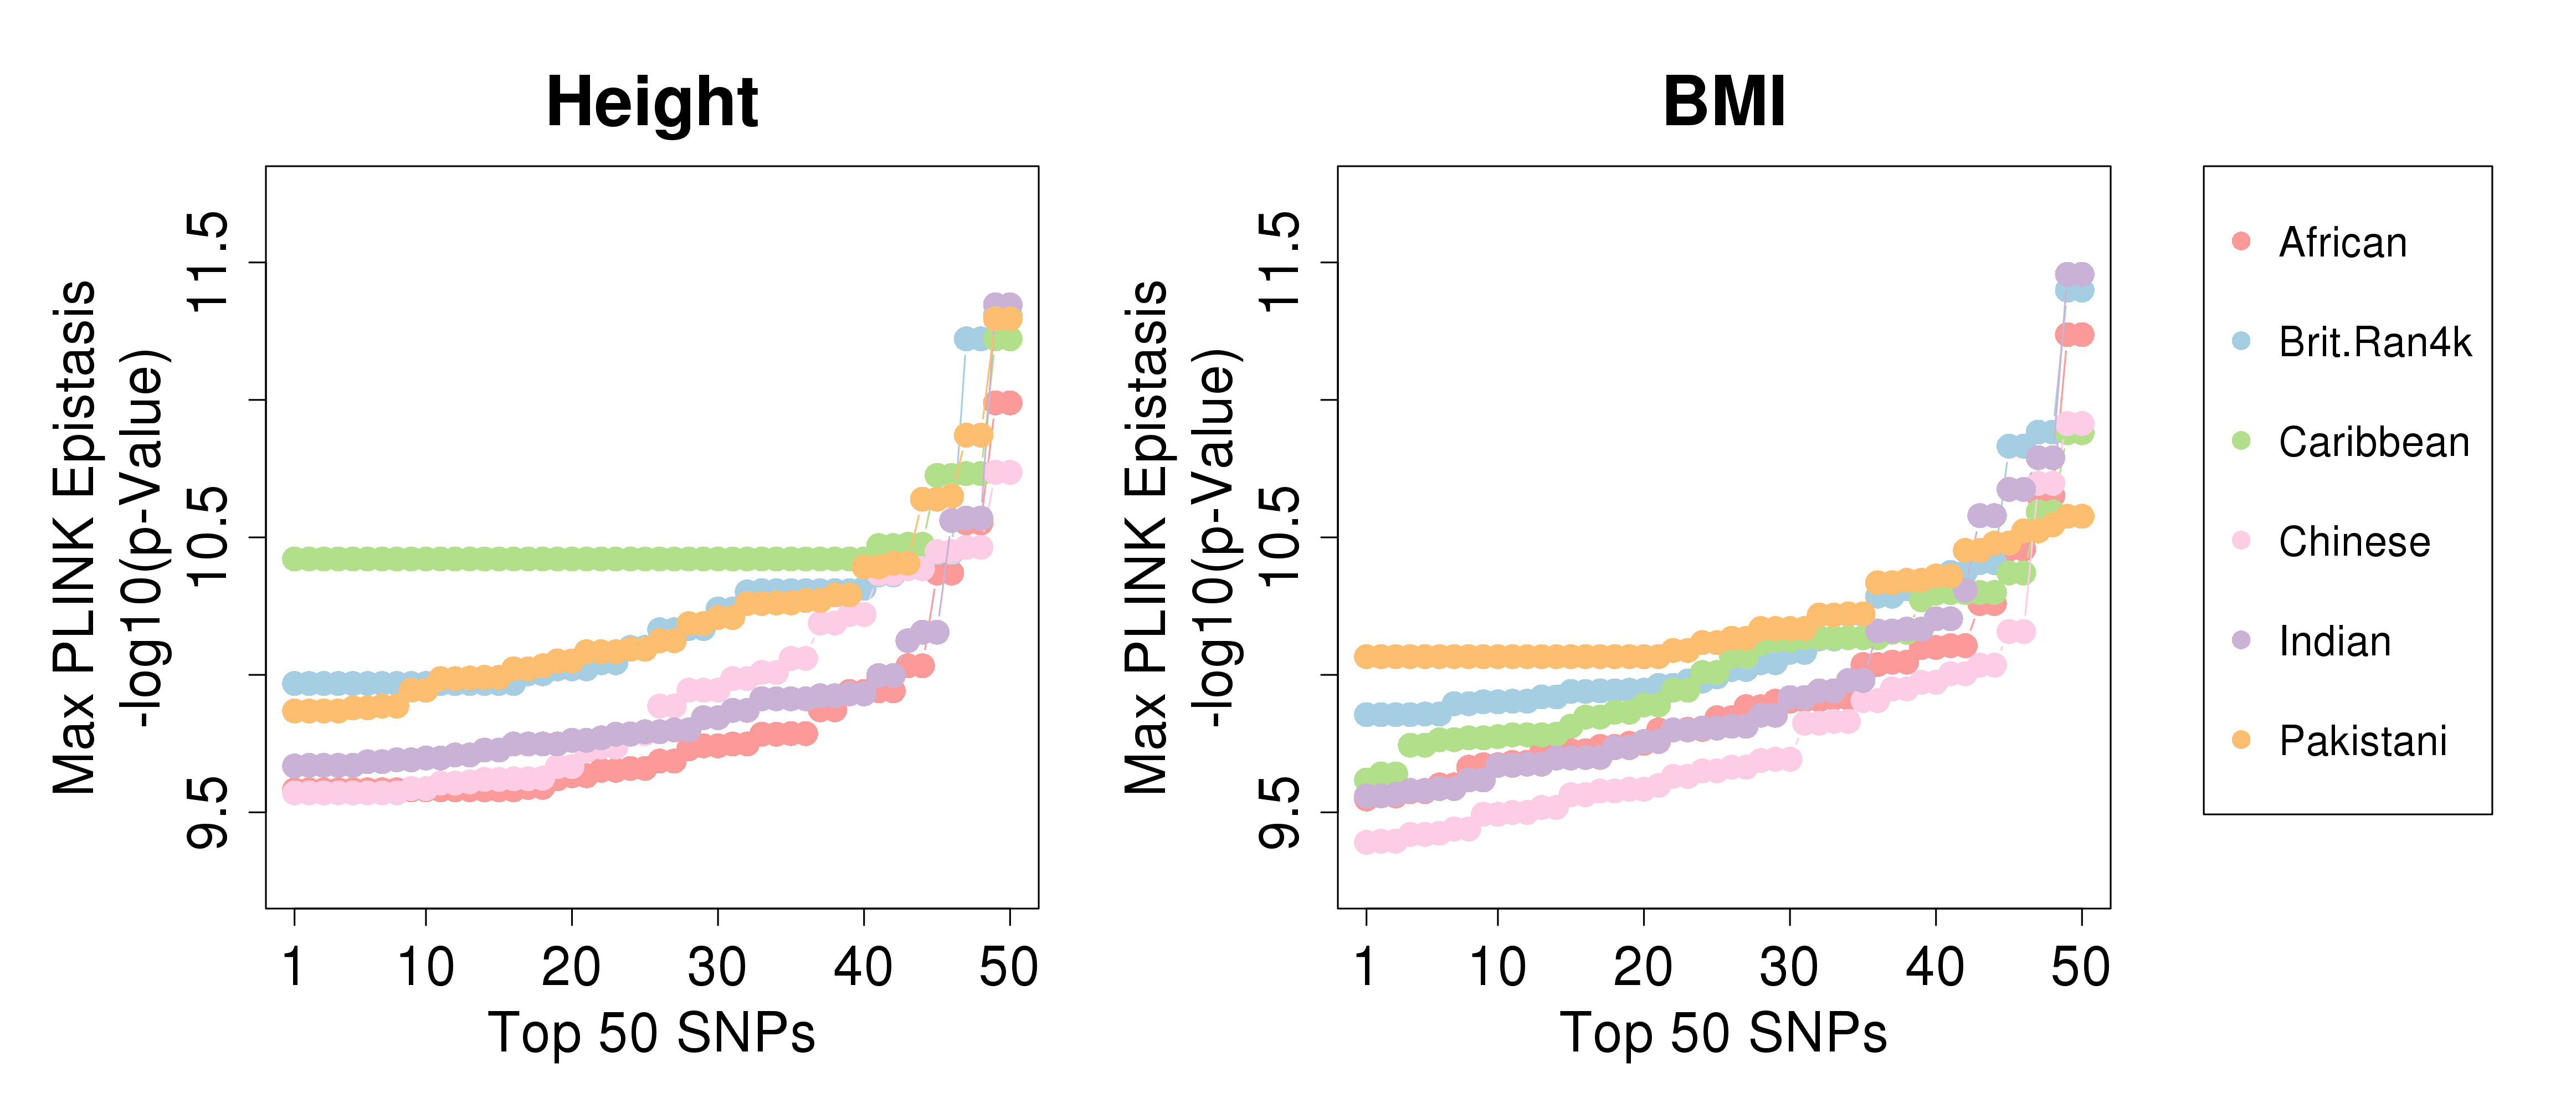
\includegraphics[scale=.45]{Images/Supp/InterPath_Supp_Figure_PLINK_BestSNPs_vs2_AllPops_HeightBMI.png}
\caption[TBD]{\textbf{PLINK Results: Top Epistasis $p$-Values }. The figure shows the best $p$-values obtained from running PLINK's exhaustive pairwise SNP epistasis test for both height and BMI in each of the UKB subsets. Only the top 50 SNPs, sorted by best pairwise SNP epistasis $p$-value, for each subset are shown. No test reaches genome-wide significance based on using a Bonferroni-corrected $p$-value threshold ($p$-value $<= 5\times10^{-13}$).}
\label{InterPath-Supp-Figure-PLINK-HeightBMI-AllPops}
\end{figure}
\clearpage

%\begin{figure}[htbp]
%\centering
%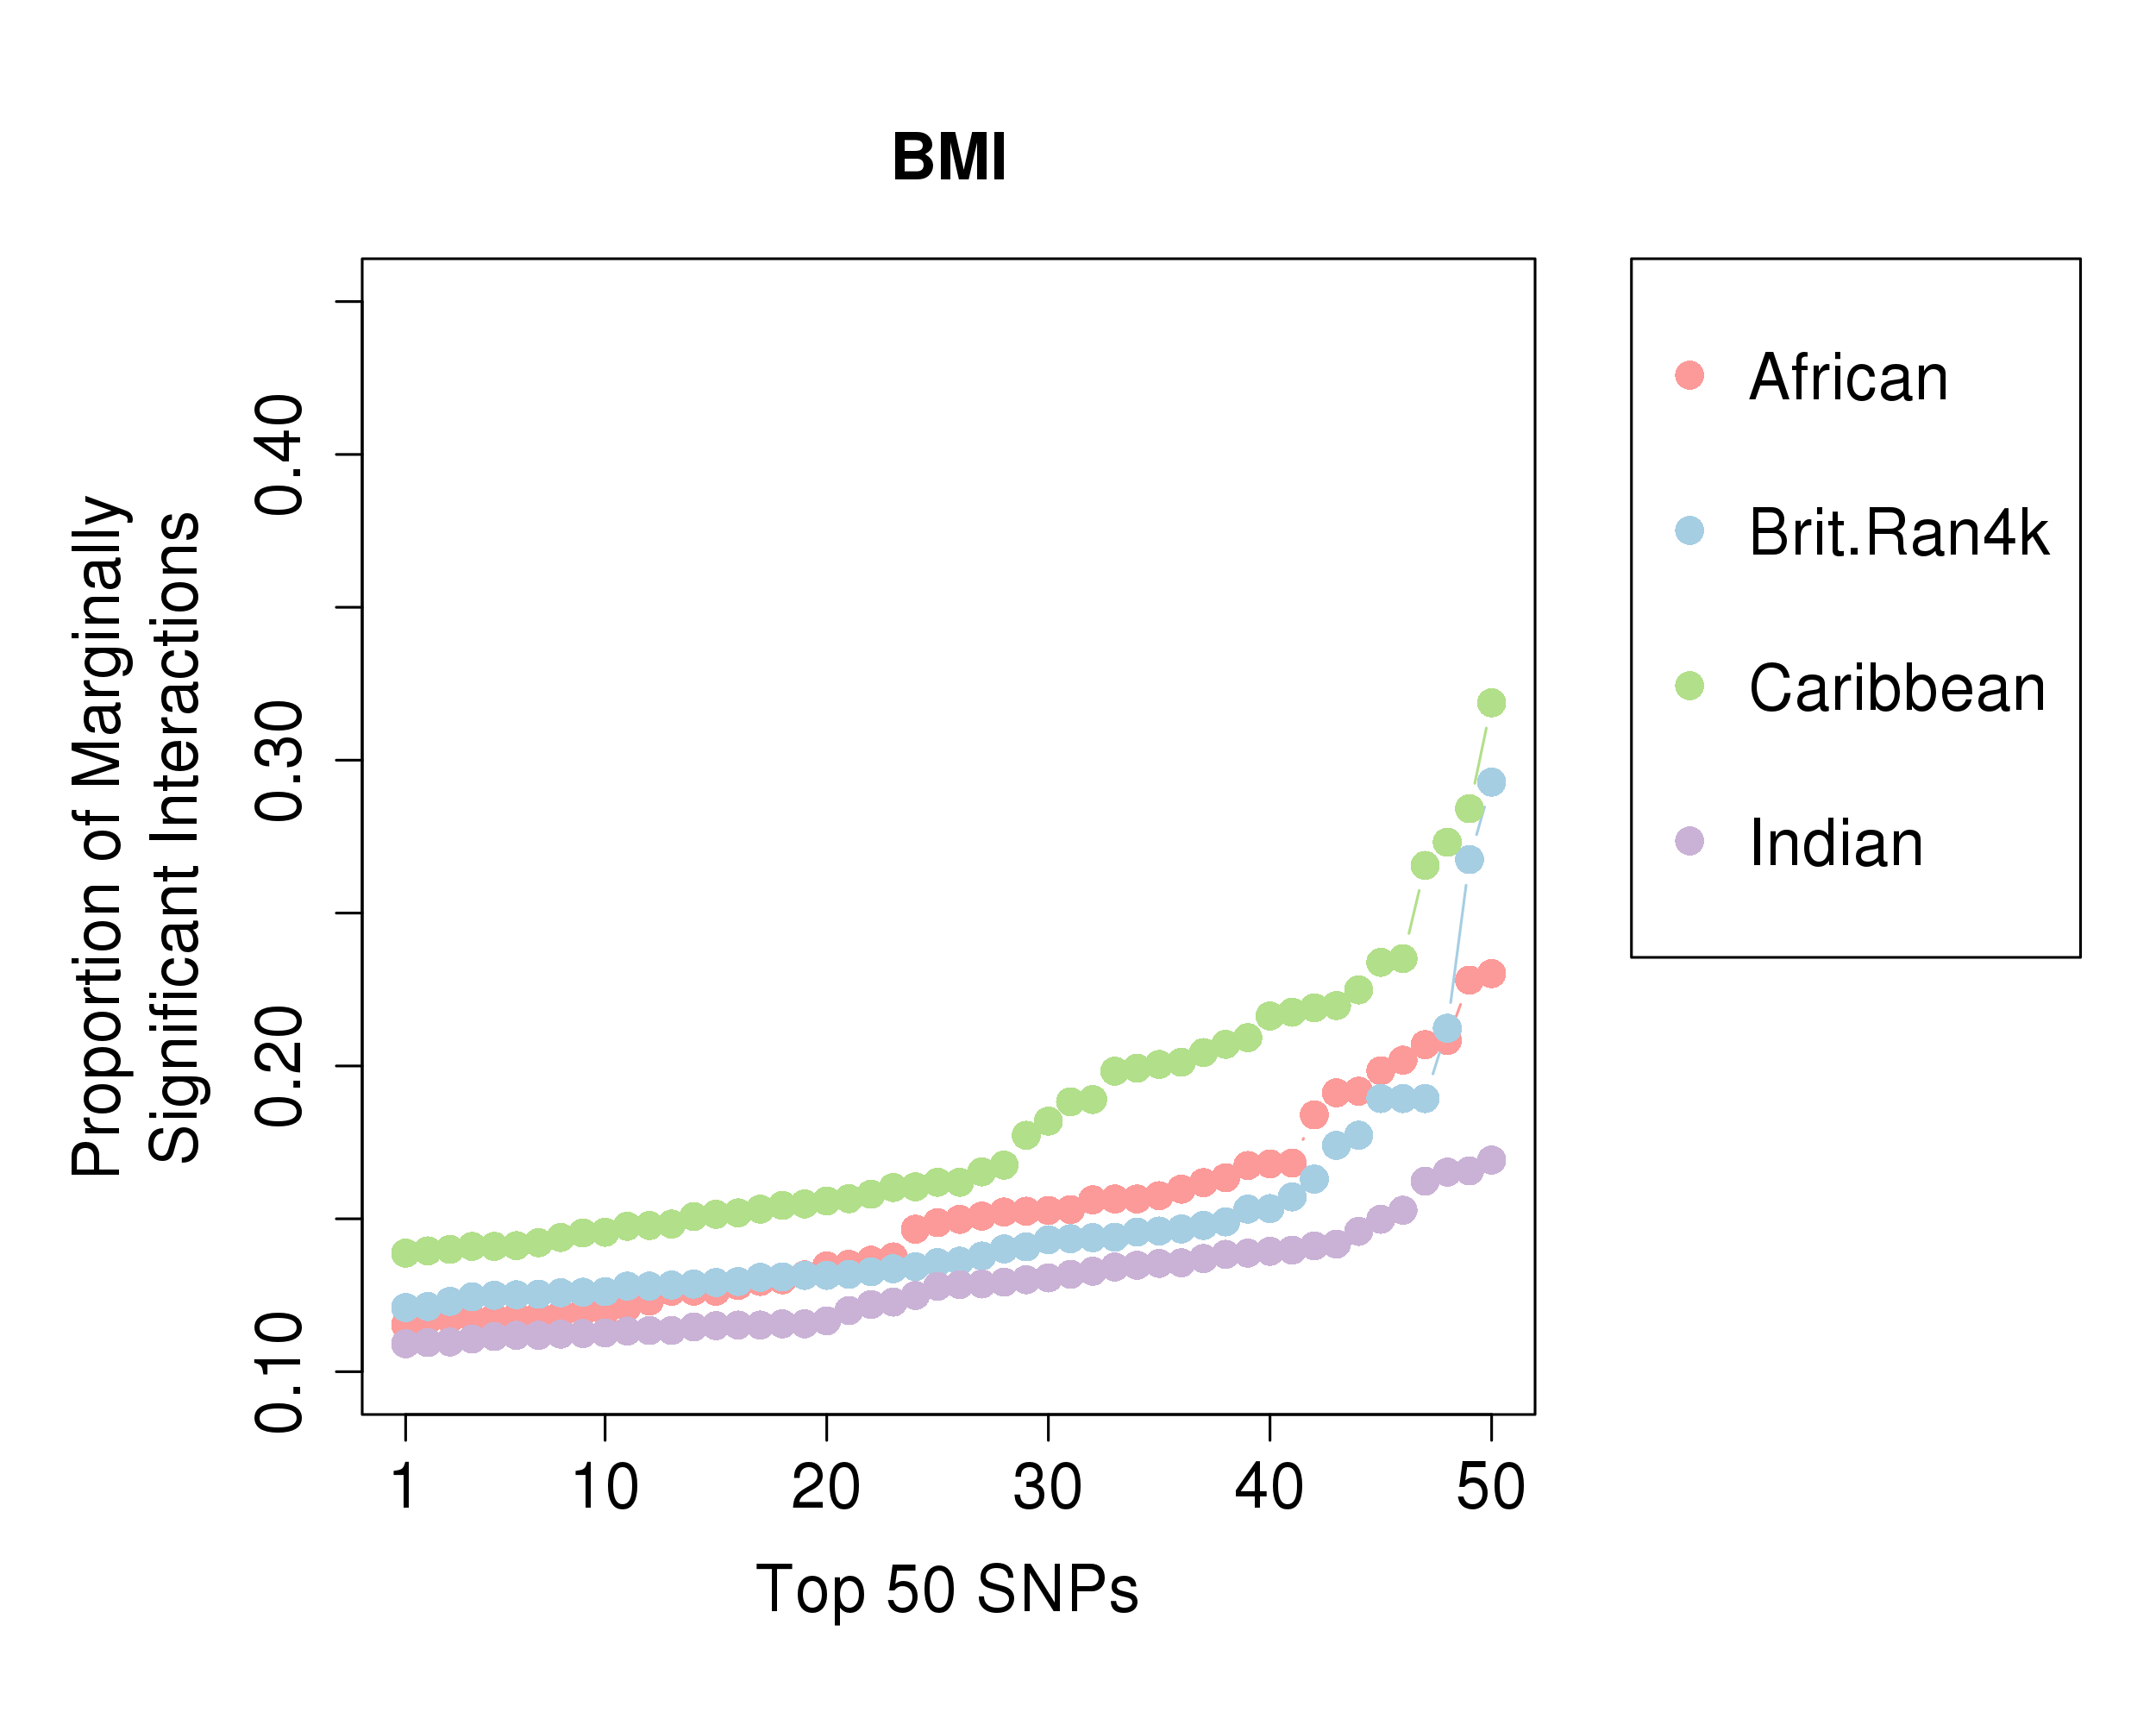
\includegraphics[scale=.5]{Images/Supp/InterPath_Supp_Figure_PLINK_vs3_BMI.png}
%\caption[TBD]{\textbf{PLINK Epistasis Proportion Results: BMI}. The figure shows the proportion of pairwise marginally significant epistatic interactions a single SNP contains when tested on height within our UKB subsets. Pairwise tests are conducted exhaustively for each individual SNP through PLINK. Marginally significant is defined as pairwise SNP epistasis $p$-value $<= 1\times10^{-4}$. Only the top 50 SNPs sorted by decreasing proportion are shown for each UKB subset. For results on height see Figure \ref{InterPath-Main-Figure-PLINK-Proportions-Height}. In general we find that the African and Caribbean subsets have the highest proportions of marginally significant interactions per SNP.}
%\label{InterPath-Supp-Figure-PLINK-Proportions-BMI}
%\end{figure}

%\begin{figure}[htbp]
%\centering
%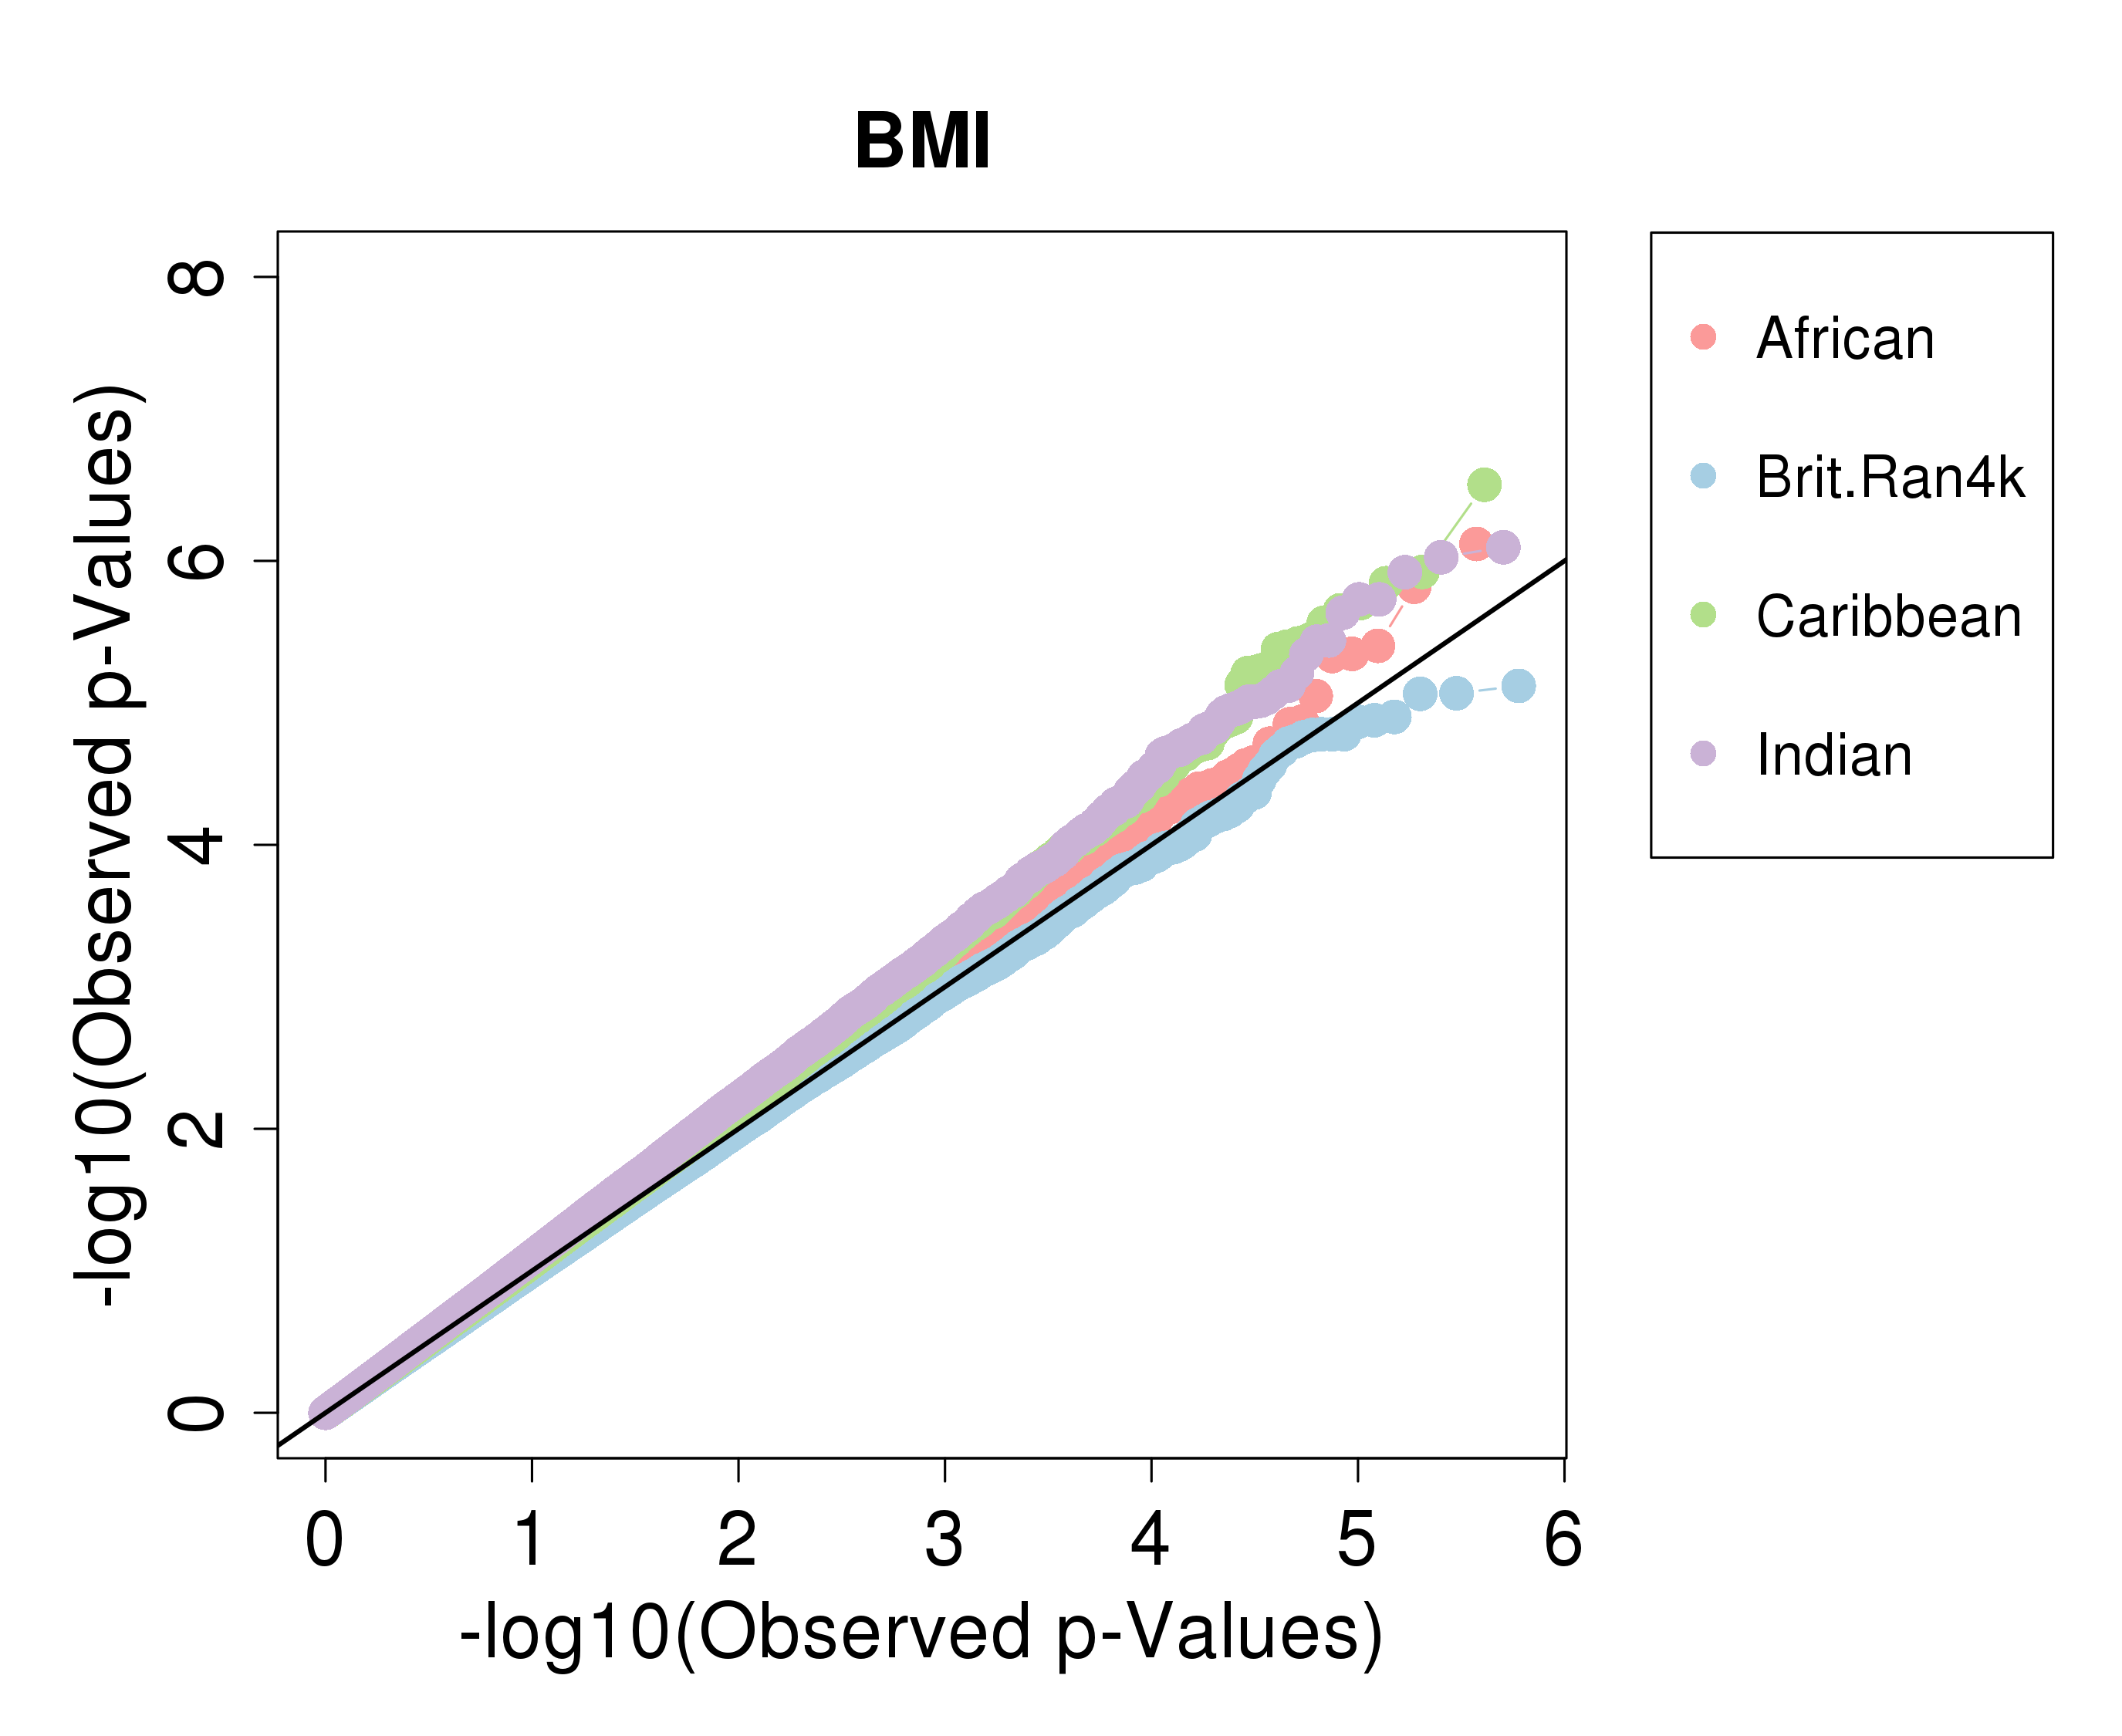
\includegraphics[scale=.5]{Images/Supp/InterPath_Supp_Figure_MAPIT_vs3_BMI.png}
%\caption[TBD]{\textbf{MAPIT Results: BMI QQ-Plots}. The figure shows QQ-plots of our results from running MAPIT on our four initial UKB population subsets in BMI. On the $x$-axis are the -$\log_{10}$ of our expected $p$-values and the on the $y$-axis are on the -$\log_{10}$ of our observed $p$-values. Each data point is a SNP and total SNP counts per UKB subset can be found in Supplementary Table \ref{InterPath-Supp-Table-UKBPopStats}.}
%\label{InterPath-Supp-Figure-MAPIT-BMI}
%\end{figure}
%\clearpage

%\begin{figure}[htbp]
%\centering
%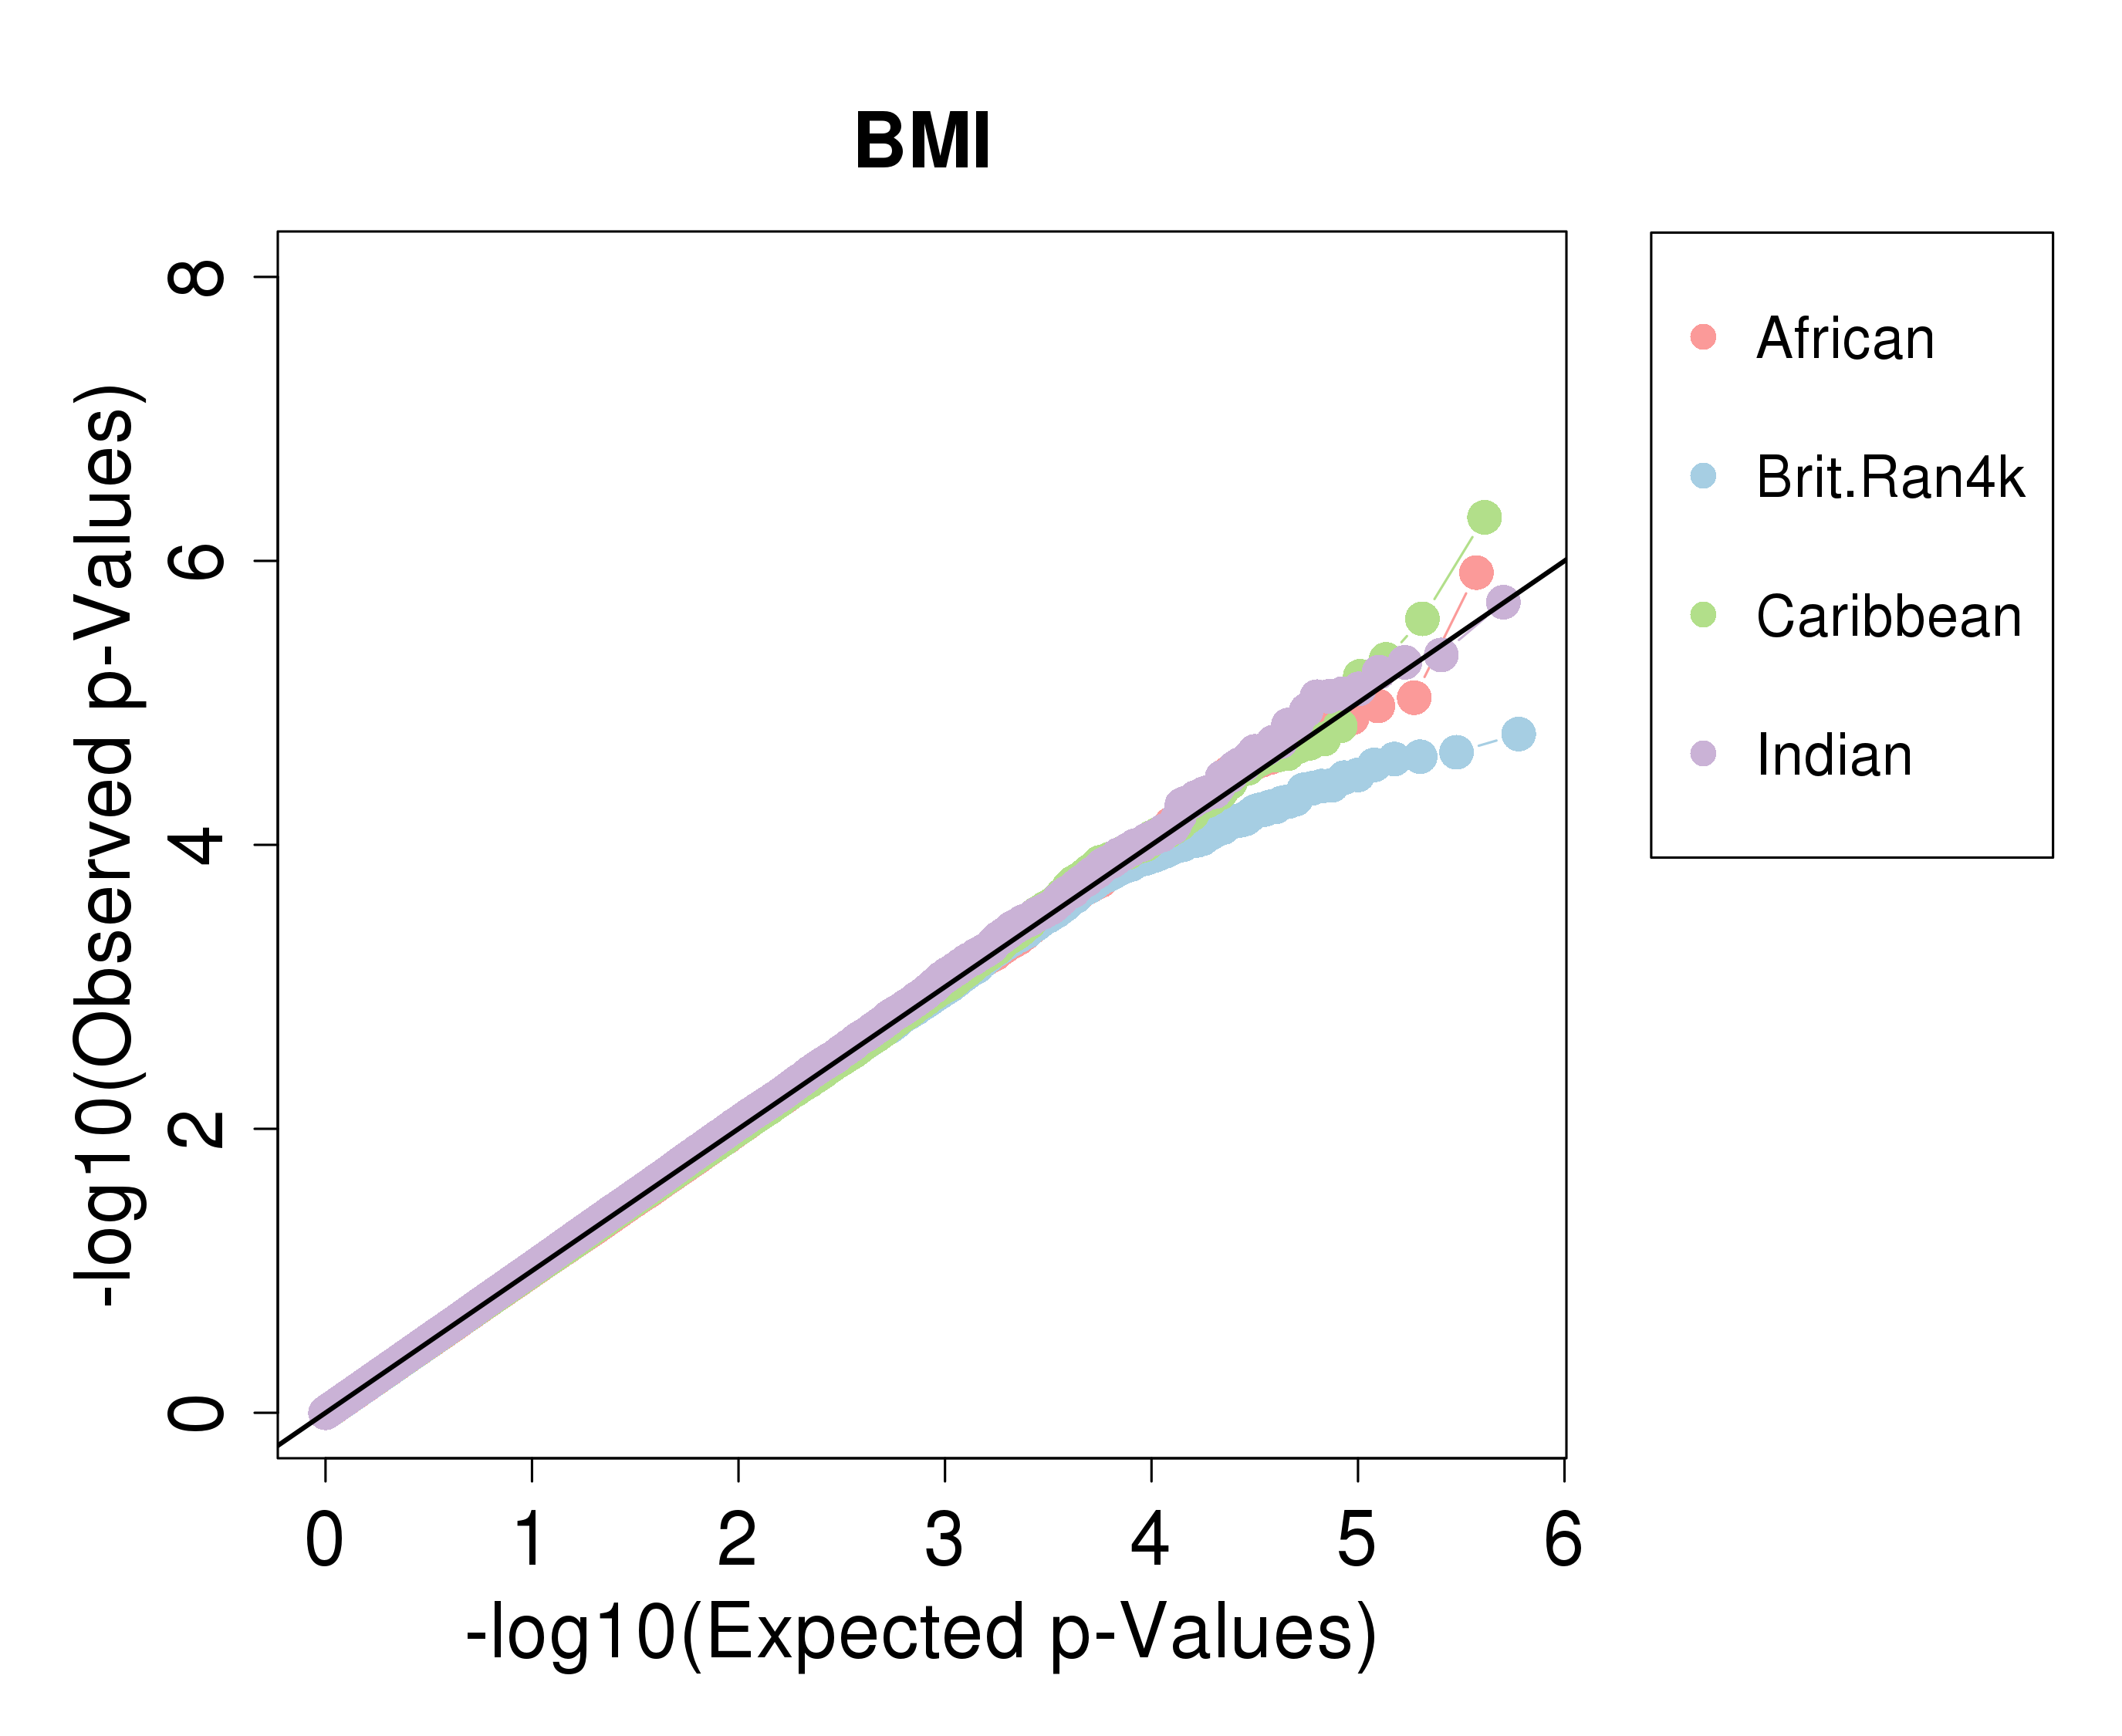
\includegraphics[scale=.35]{Images/Supp/InterPath_Supp_Figure_GWAS_vs2_BMI.png}
%\caption[TBD]{\textbf{GWAS Results QQ-Plots}.}
%\label{InterPath-Supp-Figure-GWAS-BMI}
%\end{figure}
%\clearpage
%
%\begin{figure}[htbp]
%\centering
%\hspace*{-.75cm}
%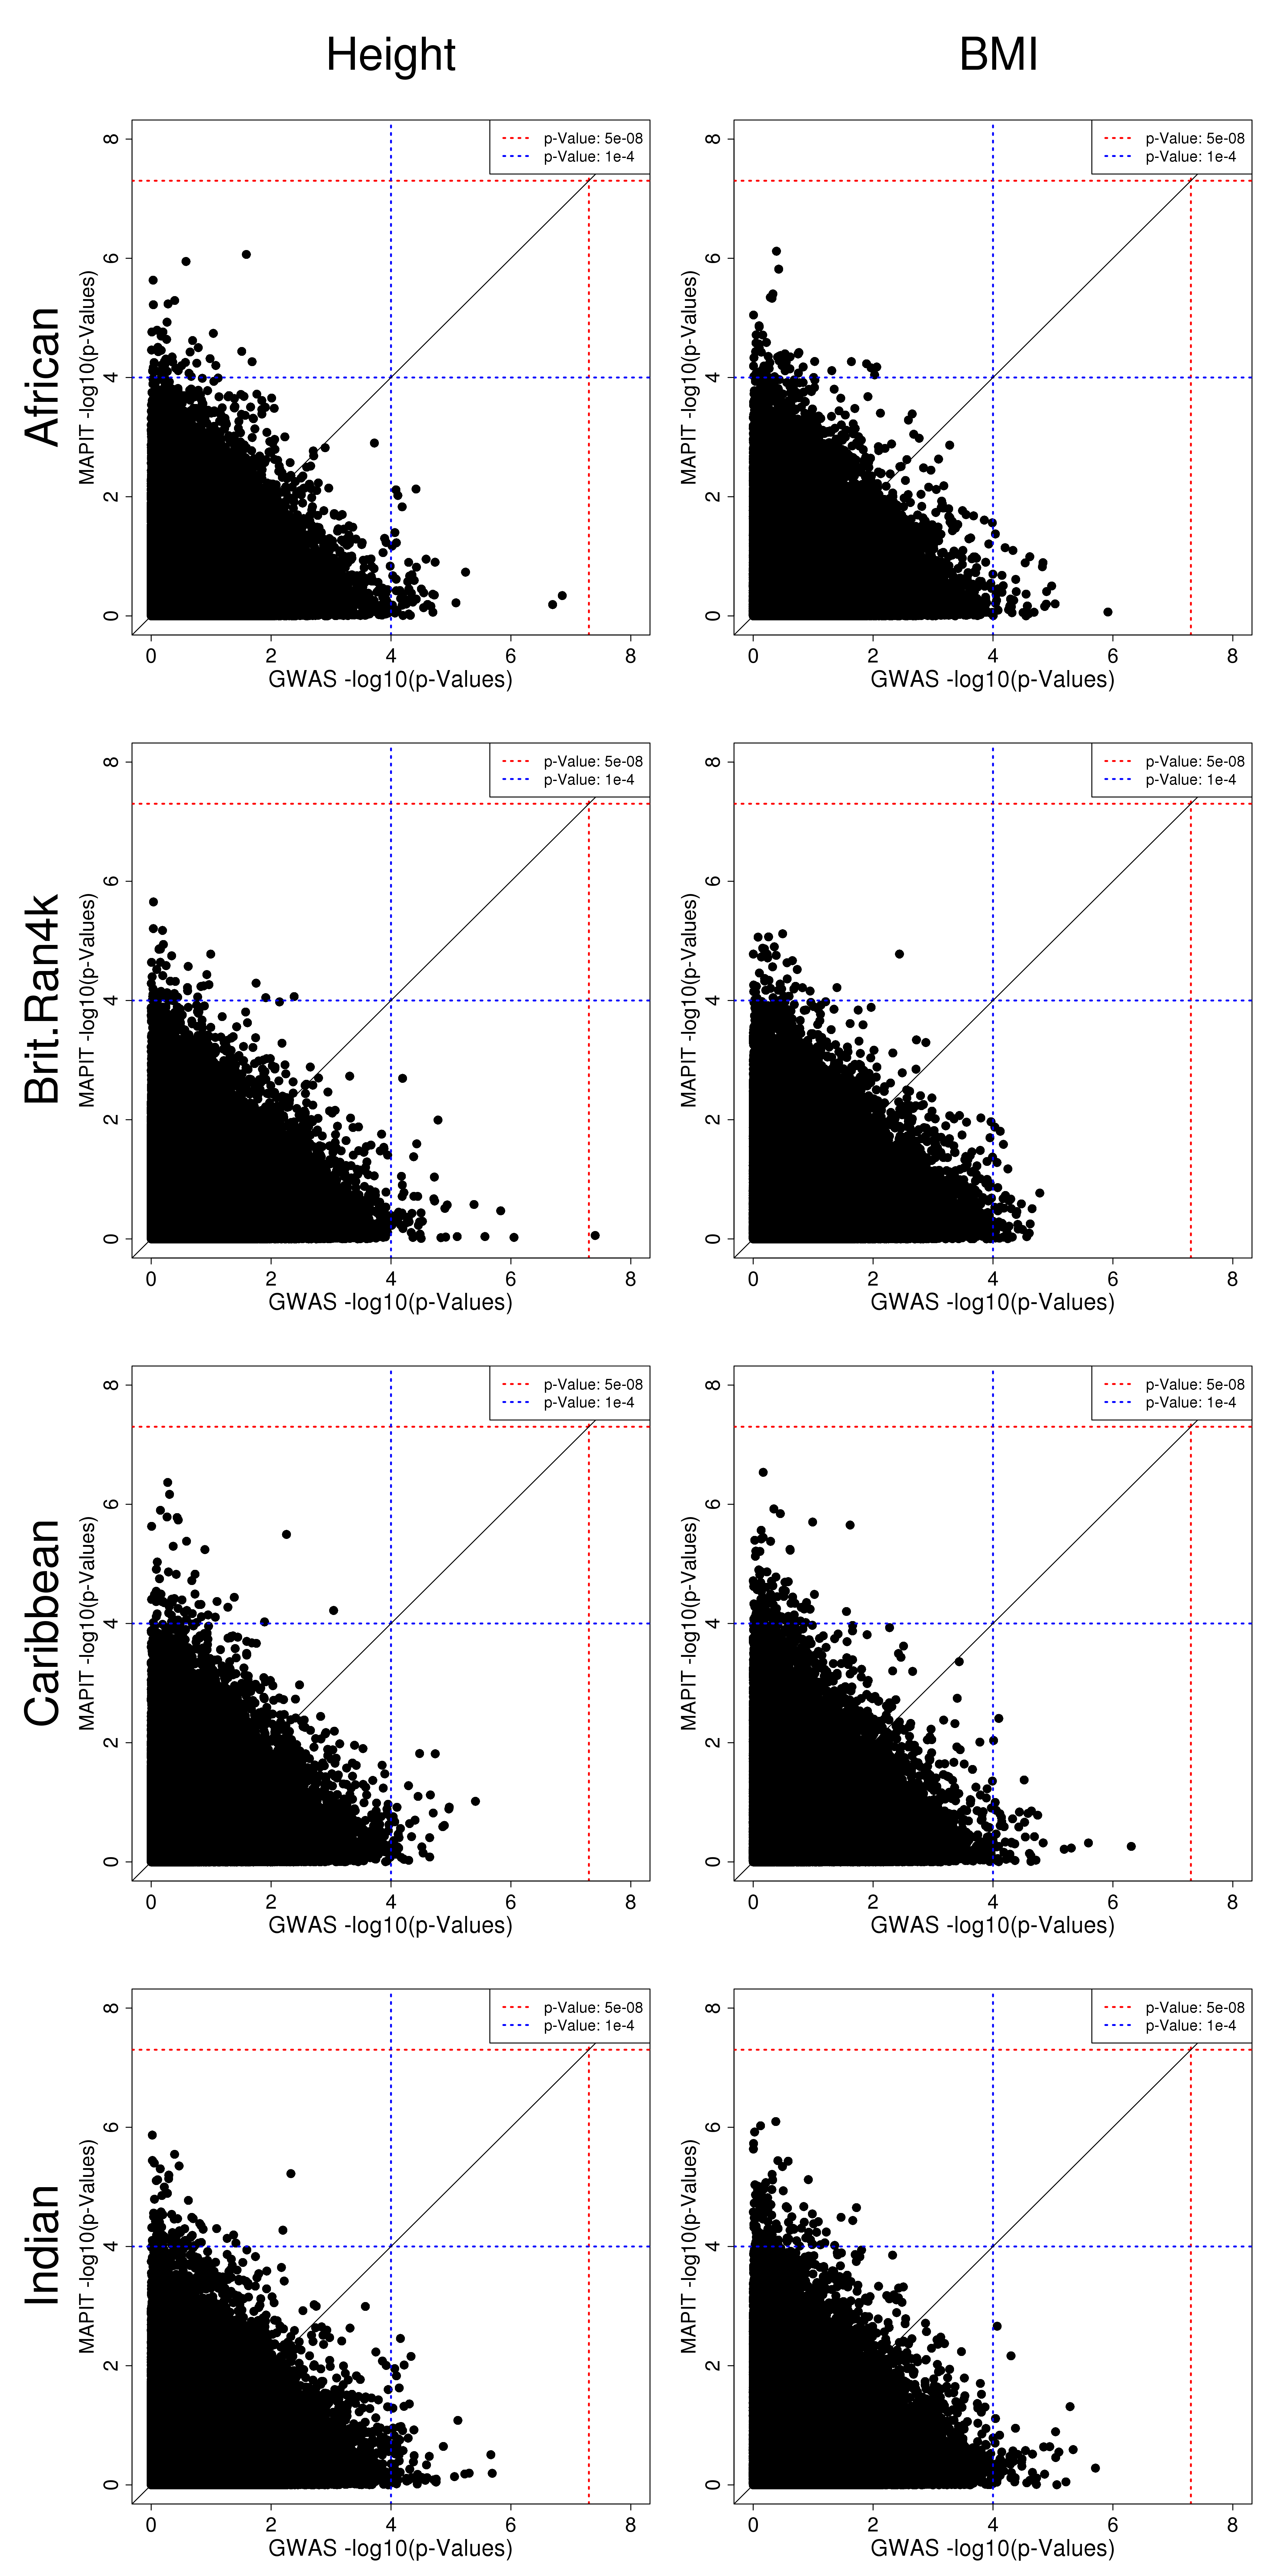
\includegraphics[scale=.3]{Images/Supp/InterPath_Supp_Figure_MAPITvsGWAS_vs2.png}
%\caption[TBD]{\textbf{MAPIT vs. GWAS Results}.}
%\label{InterPath-Supp-Figure-MAPITvsGWAS}
%\end{figure}
%\clearpage

\setlength{\footskip}{3cm}
\begin{figure}[htbp]
\centering
\vspace*{-2cm}
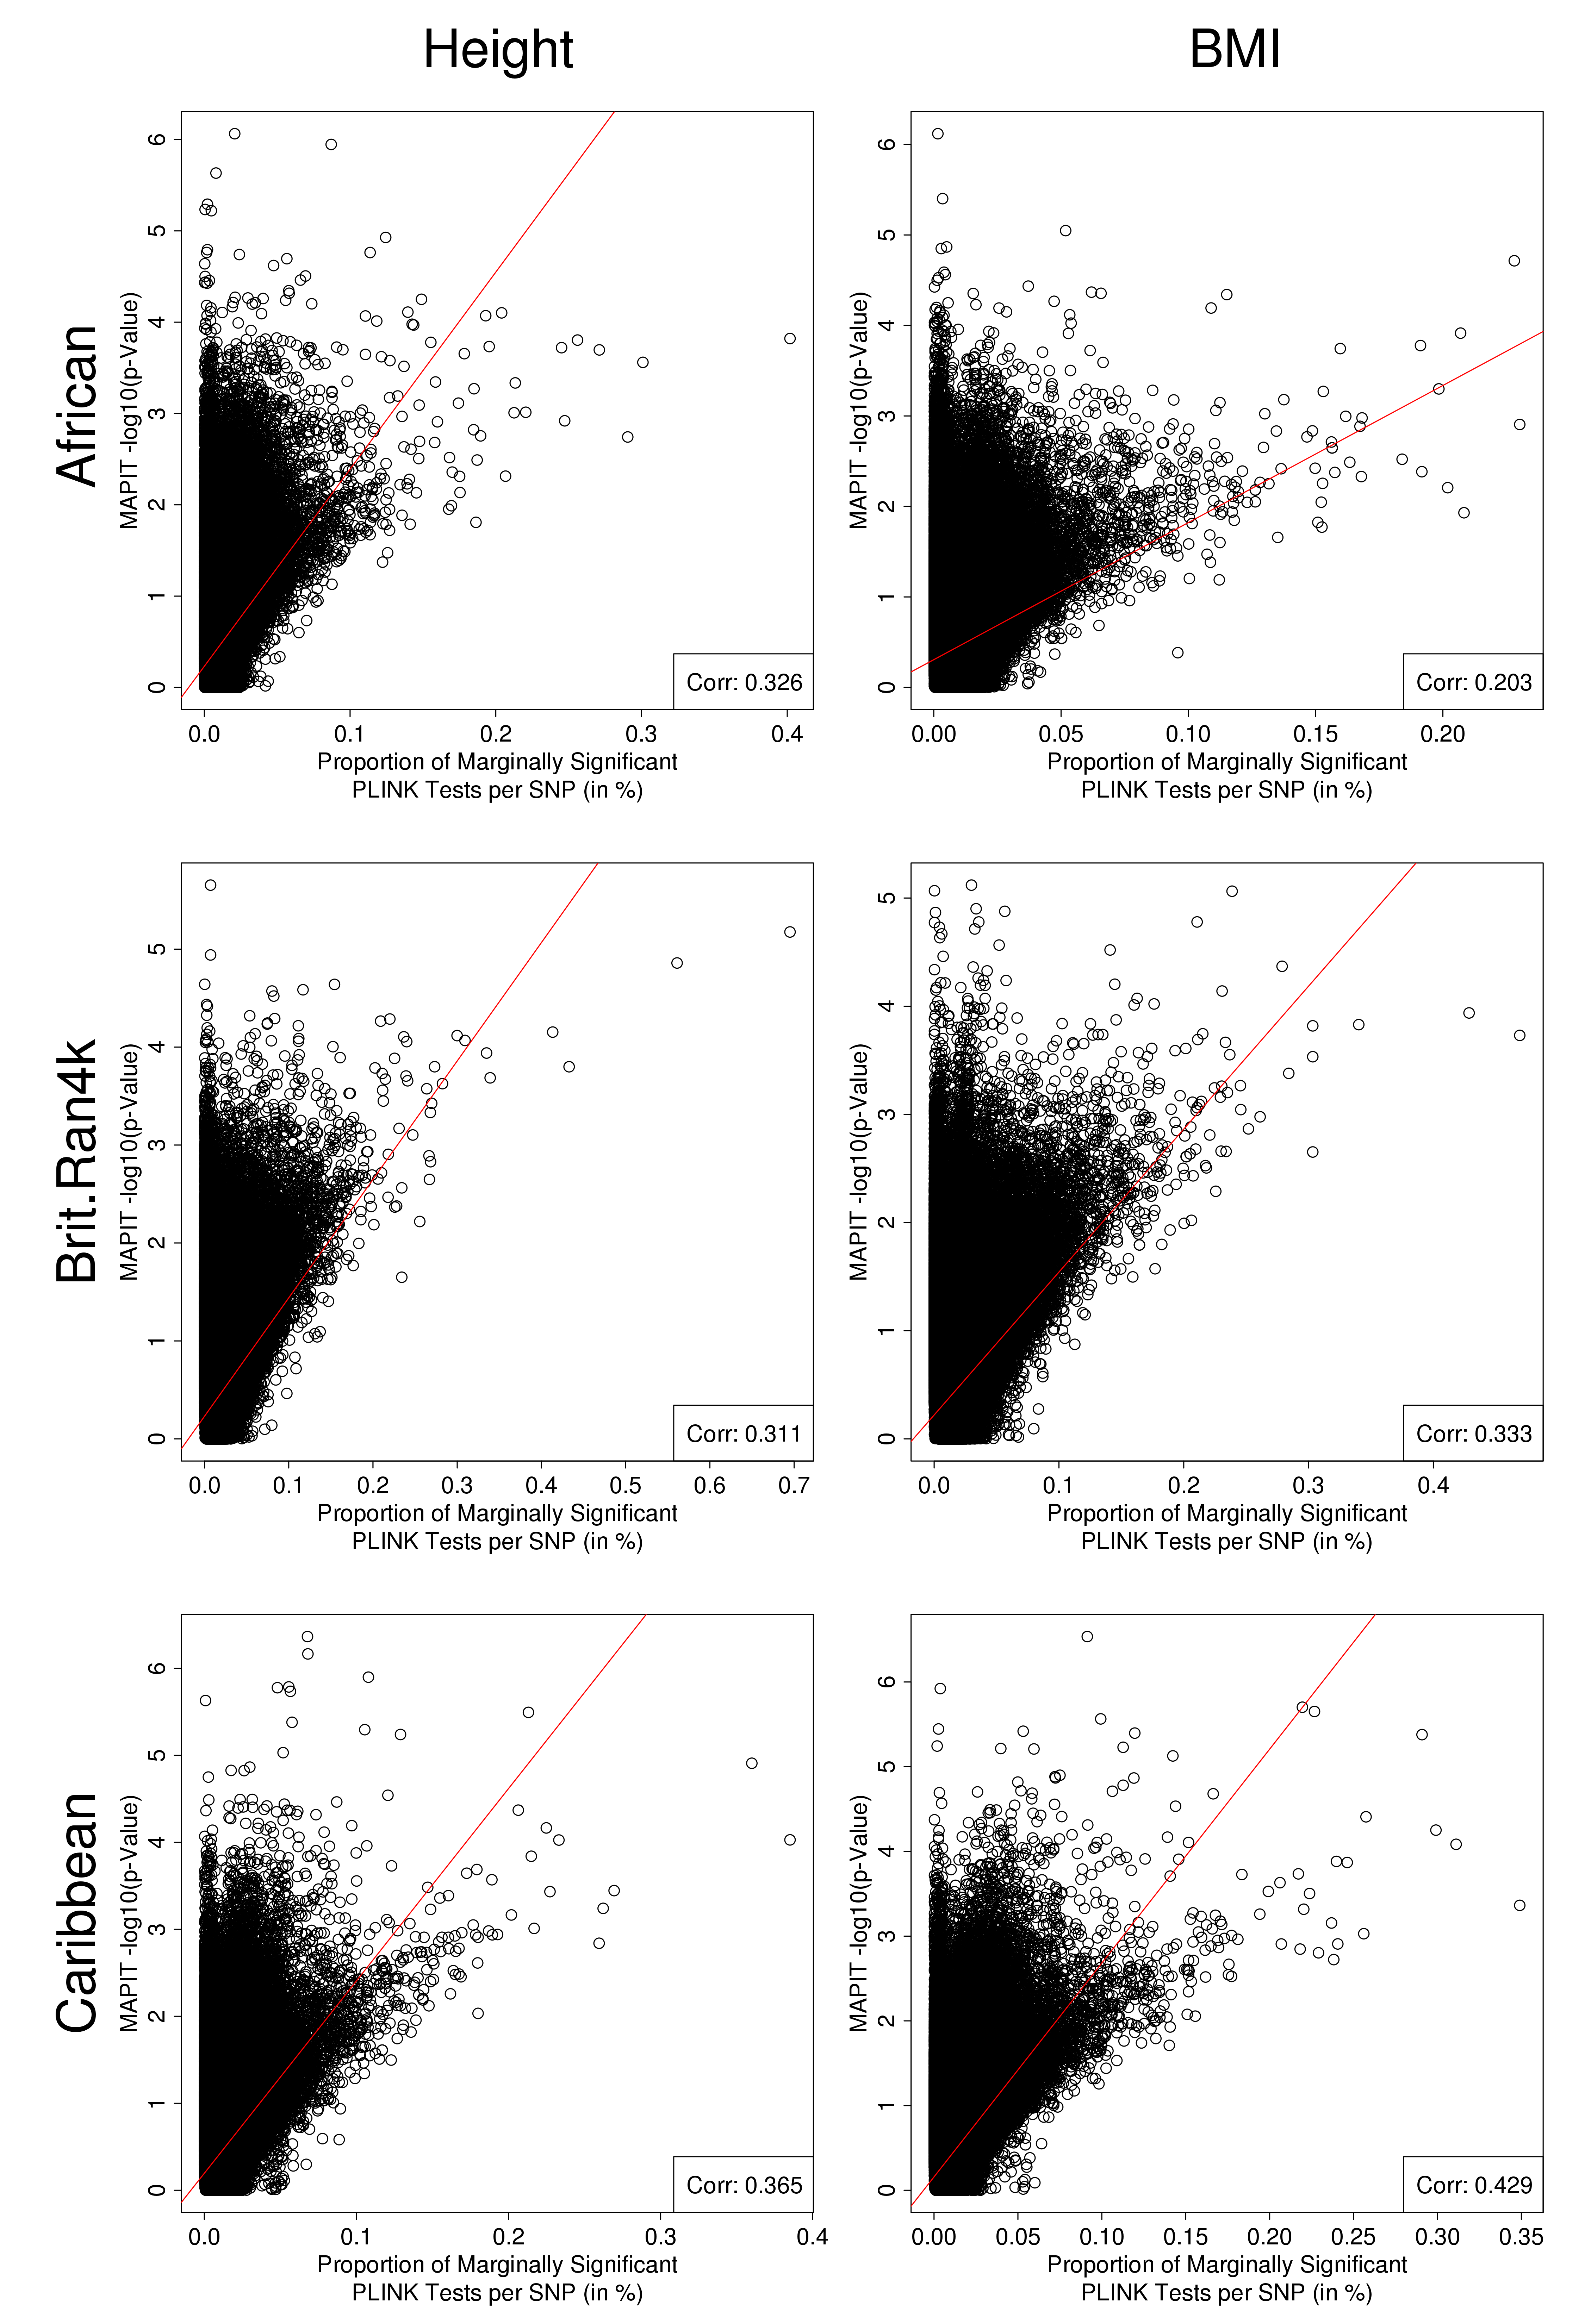
\includegraphics[scale=.3]{Images/Supp/InterPath_Supp_Figure_PLINKvsMAPIT_vs3_AllPops_HeightBMI_pt1.png}
\caption[TBD]{\textbf{PLINK vs. MAPIT: Height \& BMI in all UKB subsets}. Caption continued at end of figures.}
\label{InterPath-Supp-Figure-MAPITvsPLINK-HeightBMI-AllPops-a}
\end{figure}
\clearpage
\setlength{\footskip}{1cm}
\addtocounter{figure}{-1}

\setlength{\footskip}{3cm}
\begin{figure}[htbp]
\centering
\vspace*{-2cm}
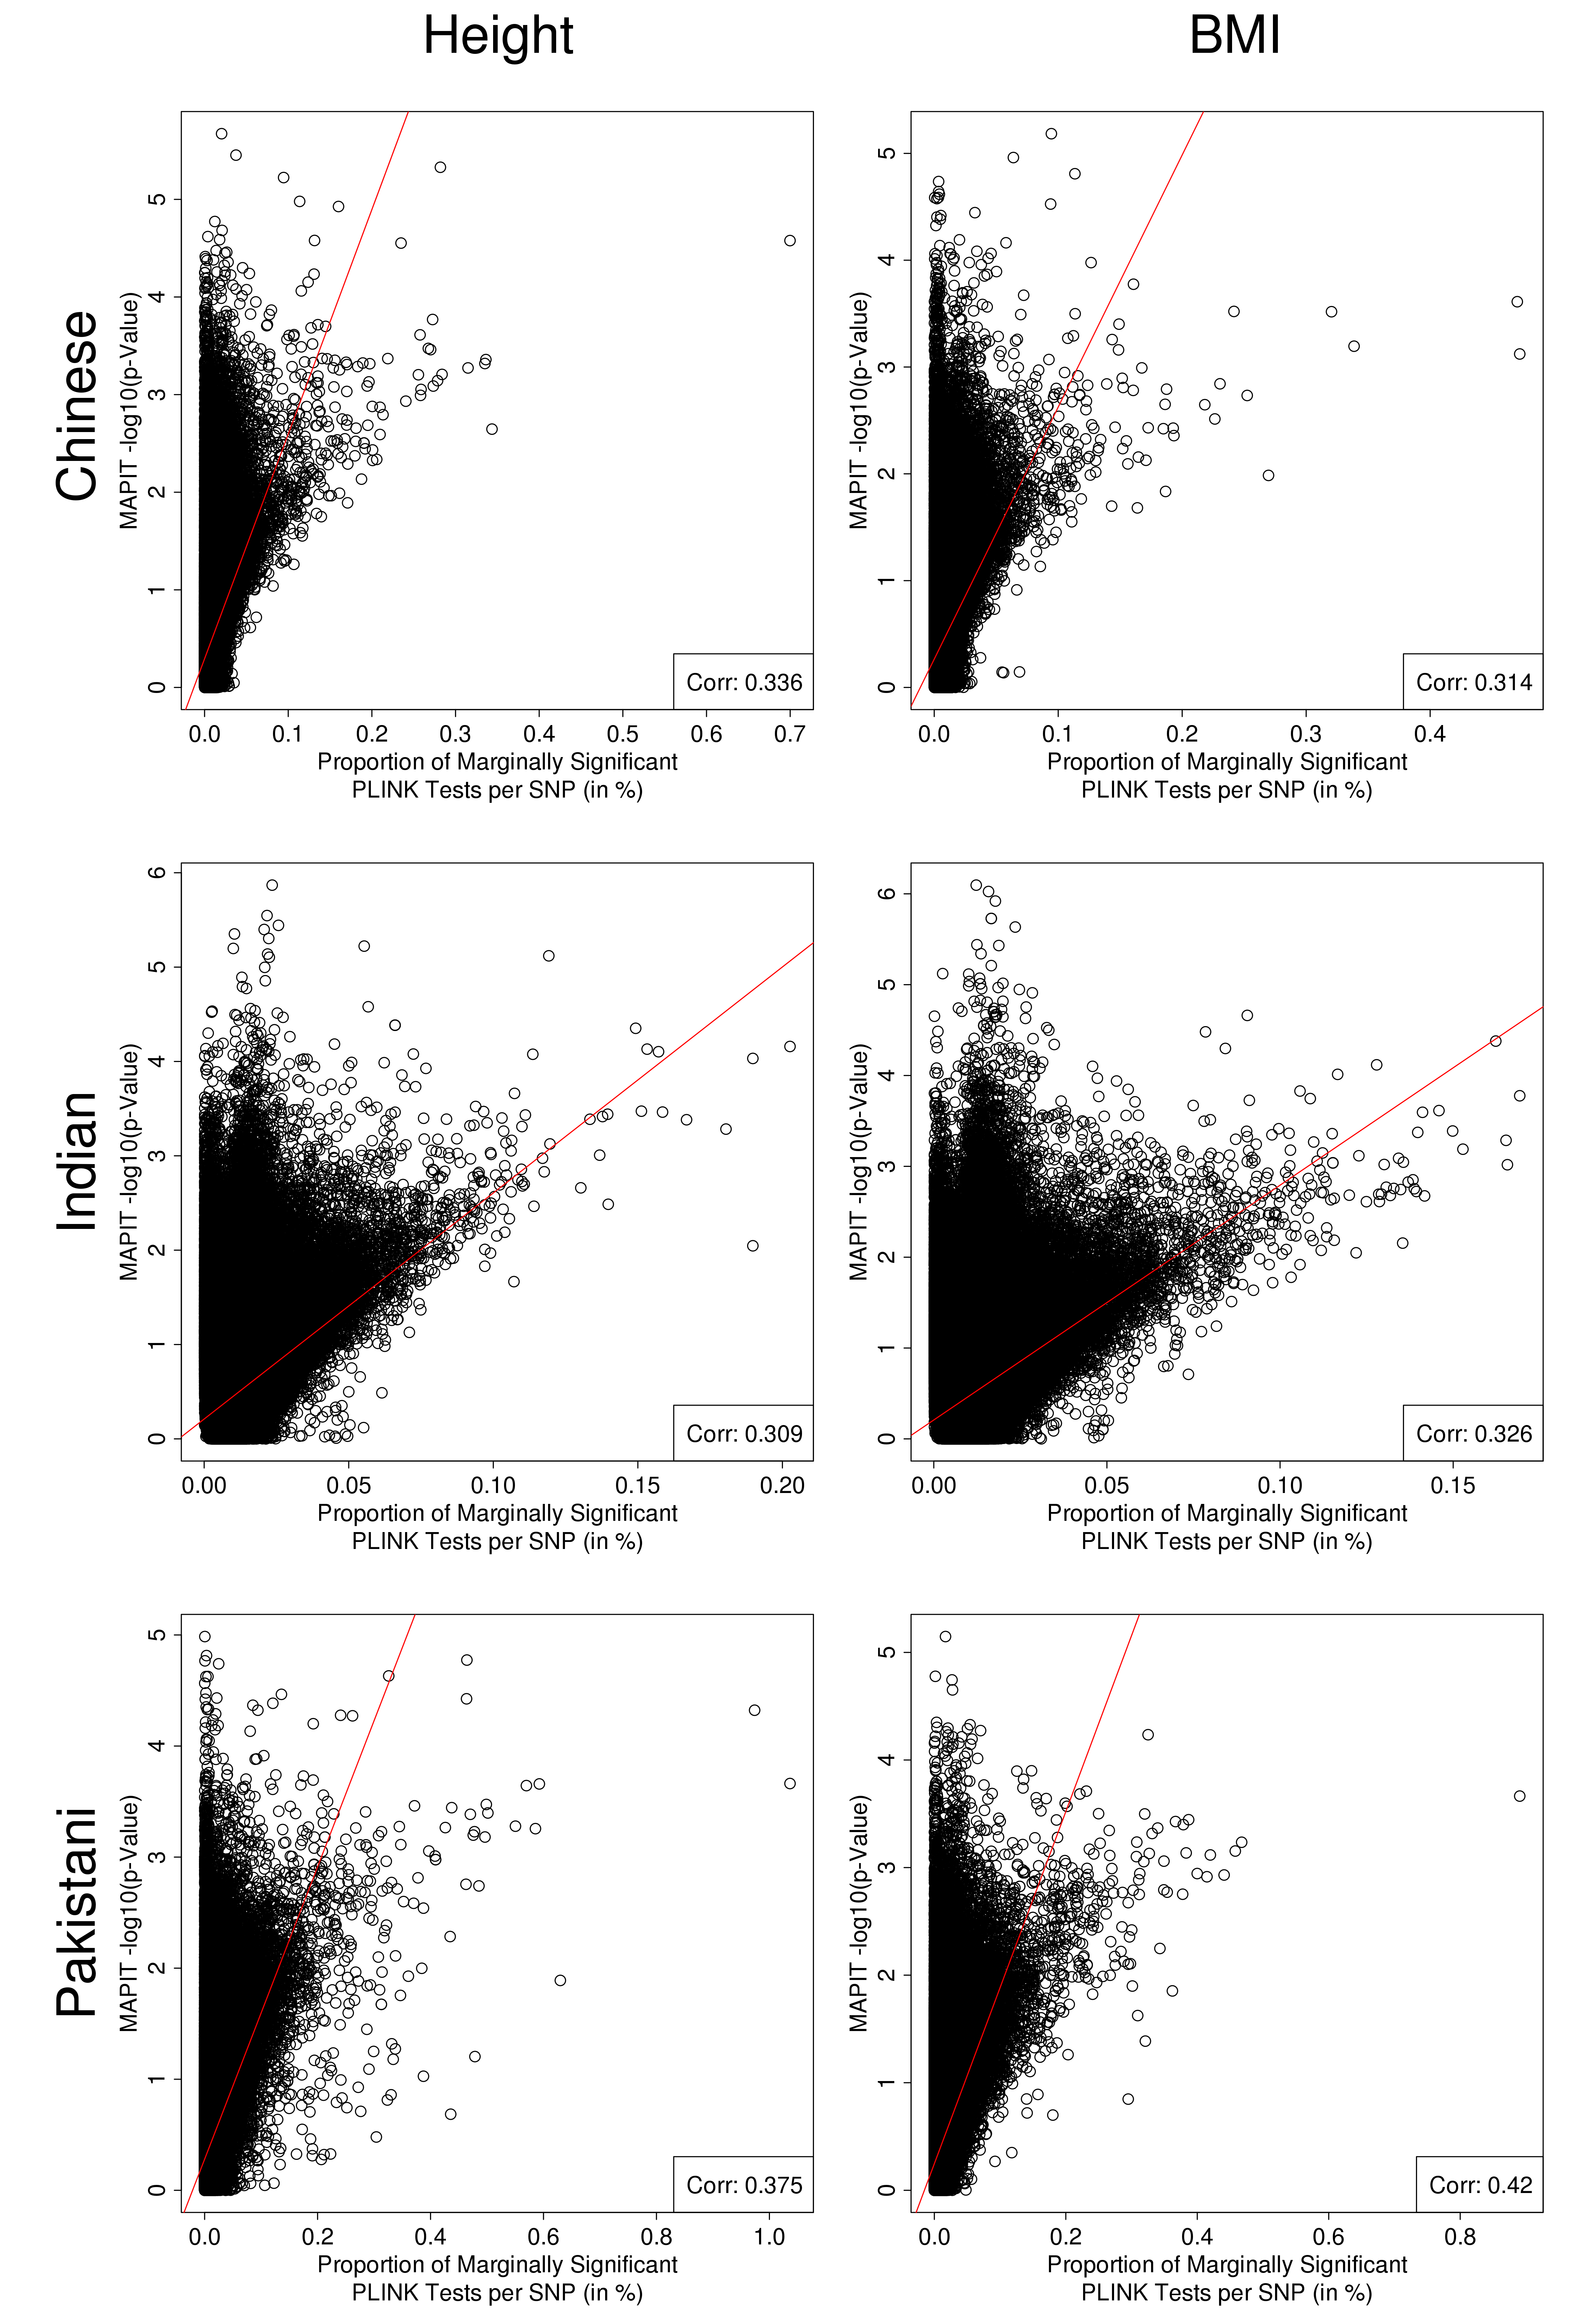
\includegraphics[scale=.3]{Images/Supp/InterPath_Supp_Figure_PLINKvsMAPIT_vs3_AllPops_HeightBMI_pt2.png}
\caption[TBD]{\textbf{PLINK vs. MAPIT: Height \& BMI in all UKB subsets}. Caption continued at end of figure.}
\label{InterPath-Supp-Figure-MAPITvsPLINK-HeightBMI-AllPops-b}
\end{figure}
\clearpage
\setlength{\footskip}{1cm}
\addtocounter{figure}{-1}

\begin{figure} [t!]
\caption[TBD]{\textbf{PLINK vs. MAPIT: Height \& BMI in all UKB subsets}. The figure shows the single-SNP PLINK results vs. MAPIT results for height and BMI in each UKB subset. For each individual plot, the PLINK results are shown on the $x$-axis as the proportion of marginally significant interactions per SNP (where marginally significant is defined as $p$-value $<= 1\times10^{-4}$) and the MAPIT results are shown on the $y$-axis as the -$\log_{10}$ of the MAPIT $p$-values. The dotted red line shows the line of best fit, and the correlation between the two metrics is shown in the legend. For many of these plots we observe a subset of SNPs with greater marginal epistasis (higher -$\log_{10}$ $p$-values) beginning to correlate with having larger proportions of marginally significant SNP-by-SNP interactions. Seeing the same signal between two different approaches suggests there may be evidence for epistasis on the single-SNP level, albeit weak.}
\label{InterPath-Supp-Figure-MAPITvsPLINK-HeightBMI-All-caption}
\end{figure}
\clearpage

\begin{figure}[htbp]
\centering
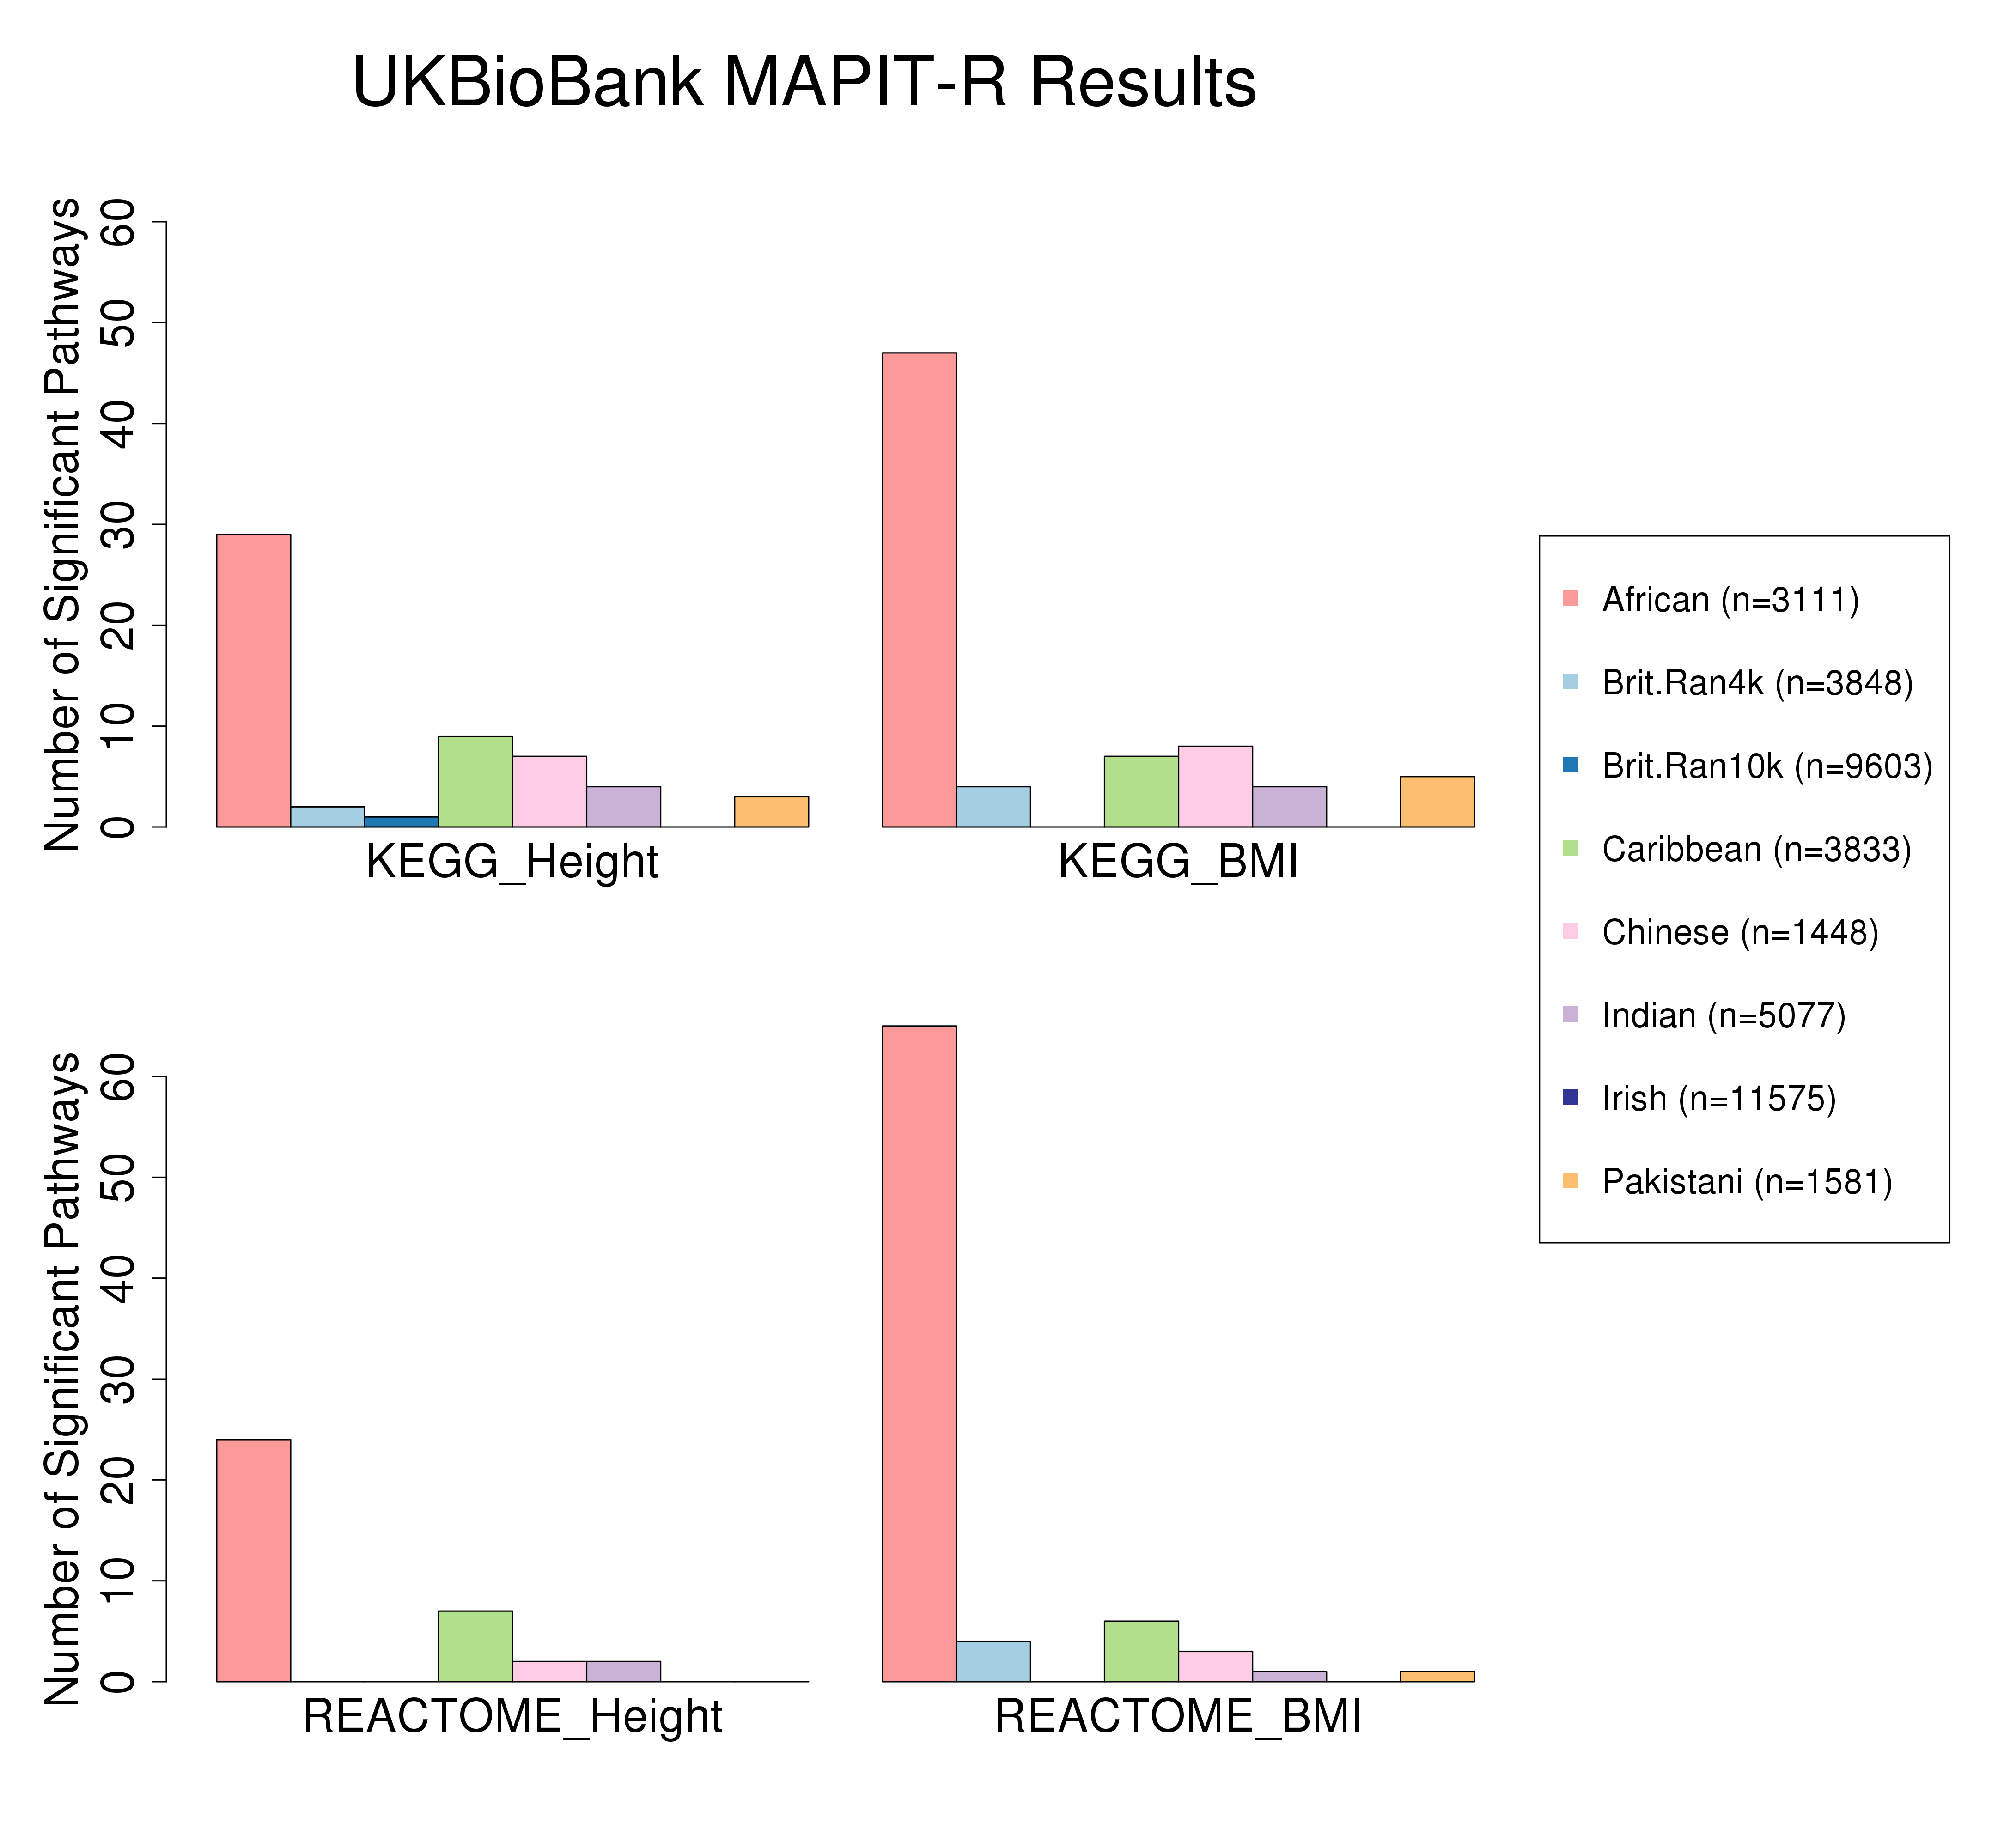
\includegraphics[scale=.35]{Images/Supp/InterPath_Supp_Figure_Barplots_vs2.png}
\caption[TBD]{\textbf{MAPIT-R Results: KEGG \& REACTOME}. The barplots show the number of genome-wide significant pathways found from running MAPIT-R for both height and BMI in the KEGG and REACTOME databases on each of our UKB subsets. Genome-wide significance was determined by using Bonferroni-corrected $p$-value thresholds based on the number of pathways tested in each phenotype, subset, and pathway database combination. As shown in these results, we find across all phenotype and database combinations that the African subset has the largest numbers of significant pathways. For lists of the specific significant pathways per subset, phenotype, and database combination, see Supplementary Tables \ref{InterPath-Supp-Table-TopPathways-KEGG-Height-a}\textcolor{blue}{-d}.}
\label{InterPath-Supp-Figure-Barplots-All}
\end{figure}
\clearpage

\begin{figure}[htbp]
\centering
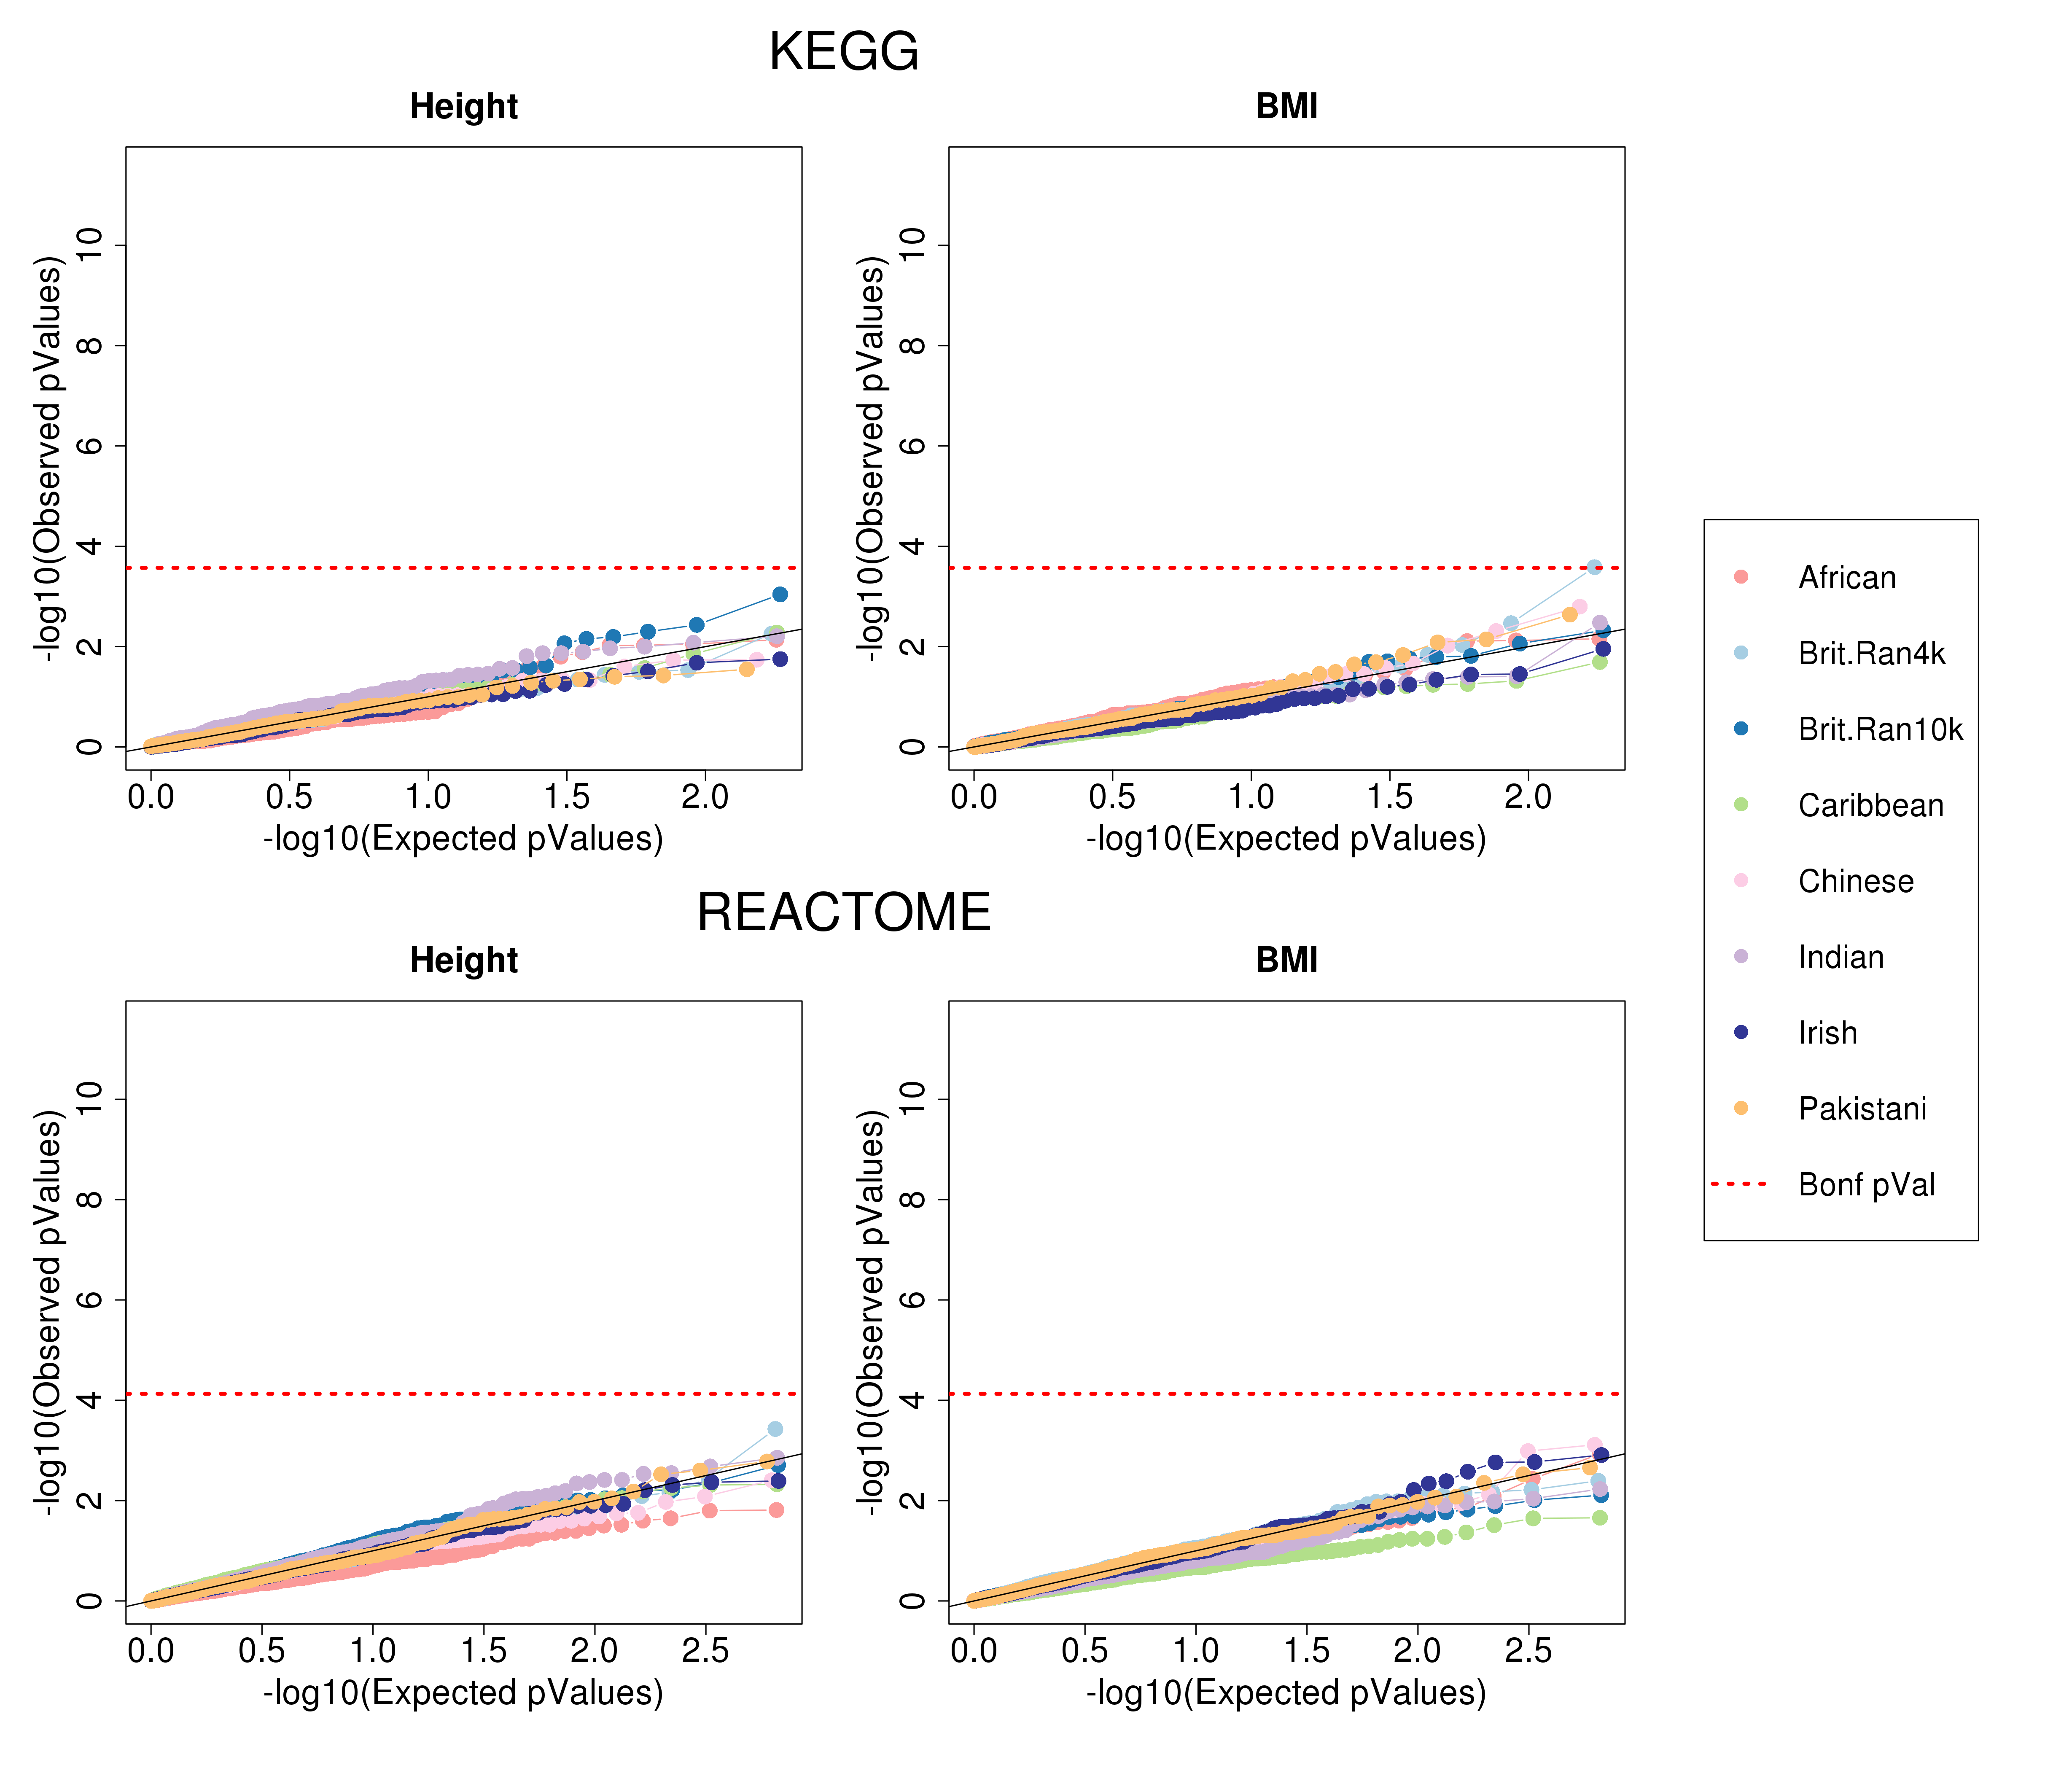
\includegraphics[scale=.35]{Images/Supp/InterPath_Supp_Figure_perm1_QQPlots_AllPaths_vs1.png}
\caption[TBD]{\textbf{MAPIT-R Results: Phenotype Permutation QQ-Plots}. The figure shows QQ-plots for running MAPIT-R using single, permuted versions of both height and BMI with the KEGG \& REACTOME databases. Phenotypes were permuted within each population subset. Shown on the $x$-axis are the -$\log_{10}$ of our expected $p$-values and the on the $y$-axis are on the -$\log_{10}$ of our observed $p$-values. The dotted red line is our Bonferroni-corrected $p$-value threshold based on the number of pathways tested per phenotype and pathway database combination. We find across all UKB subset, phenotype, and pathway database combinations that MAPIT-R displays null behavior within the range expected when using permuted phenotypes.}
\label{InterPath-Supp-Figure-perm1-QQPlots-AllPaths}
\end{figure}
\clearpage

\setlength{\footskip}{3cm}
\begin{figure}[htbp]
\centering
\vspace*{-2cm}
\includegraphics[scale=.2]{Images/Supp/InterPath_Supp_Figure_pValHists_vs3.png}
\caption[TBD]{\textbf{MAPIT-R Results: Phenotype Permutation $p$-Value Histograms}. The figure shows histograms of MAPIT-R $p$-values collected across ten independent phenotype permutation runs for each UKB subset. The same phenotype permutation for a given subset was used across both pathway databases (i.e. 10 permutations were done for height and 10 done for BMI for each subset). Covariates used from the original MAPIT-R analysis were kept the same.}
\label{InterPath-Supp-Figure-10perms-pValHists}
\end{figure}
\clearpage
\setlength{\footskip}{1cm}

\begin{figure}[htbp]
\centering
\vspace*{-2cm}
\includegraphics[scale=.15]{Images/Supp/InterPath_Supp_Figure_pValsVsNumSNPs_vs1.png}
\caption[TBD]{\textbf{MAPIT-R $p$-values Versus Number of SNPs in a Pathway}. Caption continued on next page.}
\label{InterPath-Supp-Figure-pValsVsNumSNPs}
\end{figure}
\clearpage

\addtocounter{figure}{-1}
\begin{figure} [t!]
  \caption{\textbf{MAPIT-R $p$-values Versus Number of SNPs in a Pathway}. The figure shows plots comparing the MAPIT-R $p$-values from our main analysis to the number of SNPs present in each pathway. Results for every UKB subset, phenotype, and pathway database combinations are shown. The dotted red line is the line of best fit and the legend provides the regression coefficient and its associated $p$-value. We observe that for most combinations there is a significant relationship between MAPIT-R $p$-value and the number of SNPs present in a pathway. This follows our hypothesis that combining SNPs together in a joint analysis might provide greater power to detect marginal epistasis than analyzing each SNP independently. We note, however, that these results appear to not solely be driven just by the presence or absence of large SNP counts -- conducting this same analysis on one of our sets of permuted phenotypes we now find very few significant relationships between MAPIT-R $p$-values and pathway SNP counts (Supplementary Figure \ref{InterPath-Supp-Figure-pValsVsNumSNPs-perm1}}
\label{InterPath-Supp-Figure-pValsVsNumSNPs-Caption}
\end{figure}
\clearpage

\setlength{\footskip}{3cm}
\begin{figure}[htbp]
\centering
\vspace*{-2cm}
\includegraphics[scale=.15]{Images/Supp/InterPath_Supp_Figure_pValsVsNumSNPs_perm1_vs1.png}
\caption[TBD]{\textbf{MAPIT-R $p$-values Versus Number of SNPs in a Pathway, Permuted Phenotypes}. Caption continued on next page.}
\label{InterPath-Supp-Figure-pValsVsNumSNPs-perm1}
\end{figure}
\clearpage
\setlength{\footskip}{1cm}

\addtocounter{figure}{-1}
\begin{figure} [t!]
  \caption{\textbf{MAPIT-R $p$-values Versus Number of SNPs in a Pathway, Permuted Phenotypes}. The figure shows plots comparing the MAPIT-R $p$-values from our main analysis to the number of SNPs present in each pathway. For this analysis a single set of our permuted phenotypes (i.e. Supplementary Figure \ref{InterPath-Supp-Figure-perm1-QQPlots-AllPaths}) was used for each UKB subset. Results for every subset, permuted phenotype, and pathway database combinations are shown. The dotted red line is the line of best fit and the legend provides the regression coefficient and its associated $p$-value. We observe that for very few combinations there is any relationship between MAPIT-R $p$-value and the number of SNPs present in a pathway.}
\label{InterPath-Supp-Figure-pValsVsNumSNPs-perm1-Caption}
\end{figure}
\clearpage

%\begin{figure}[htbp]
%\centering
%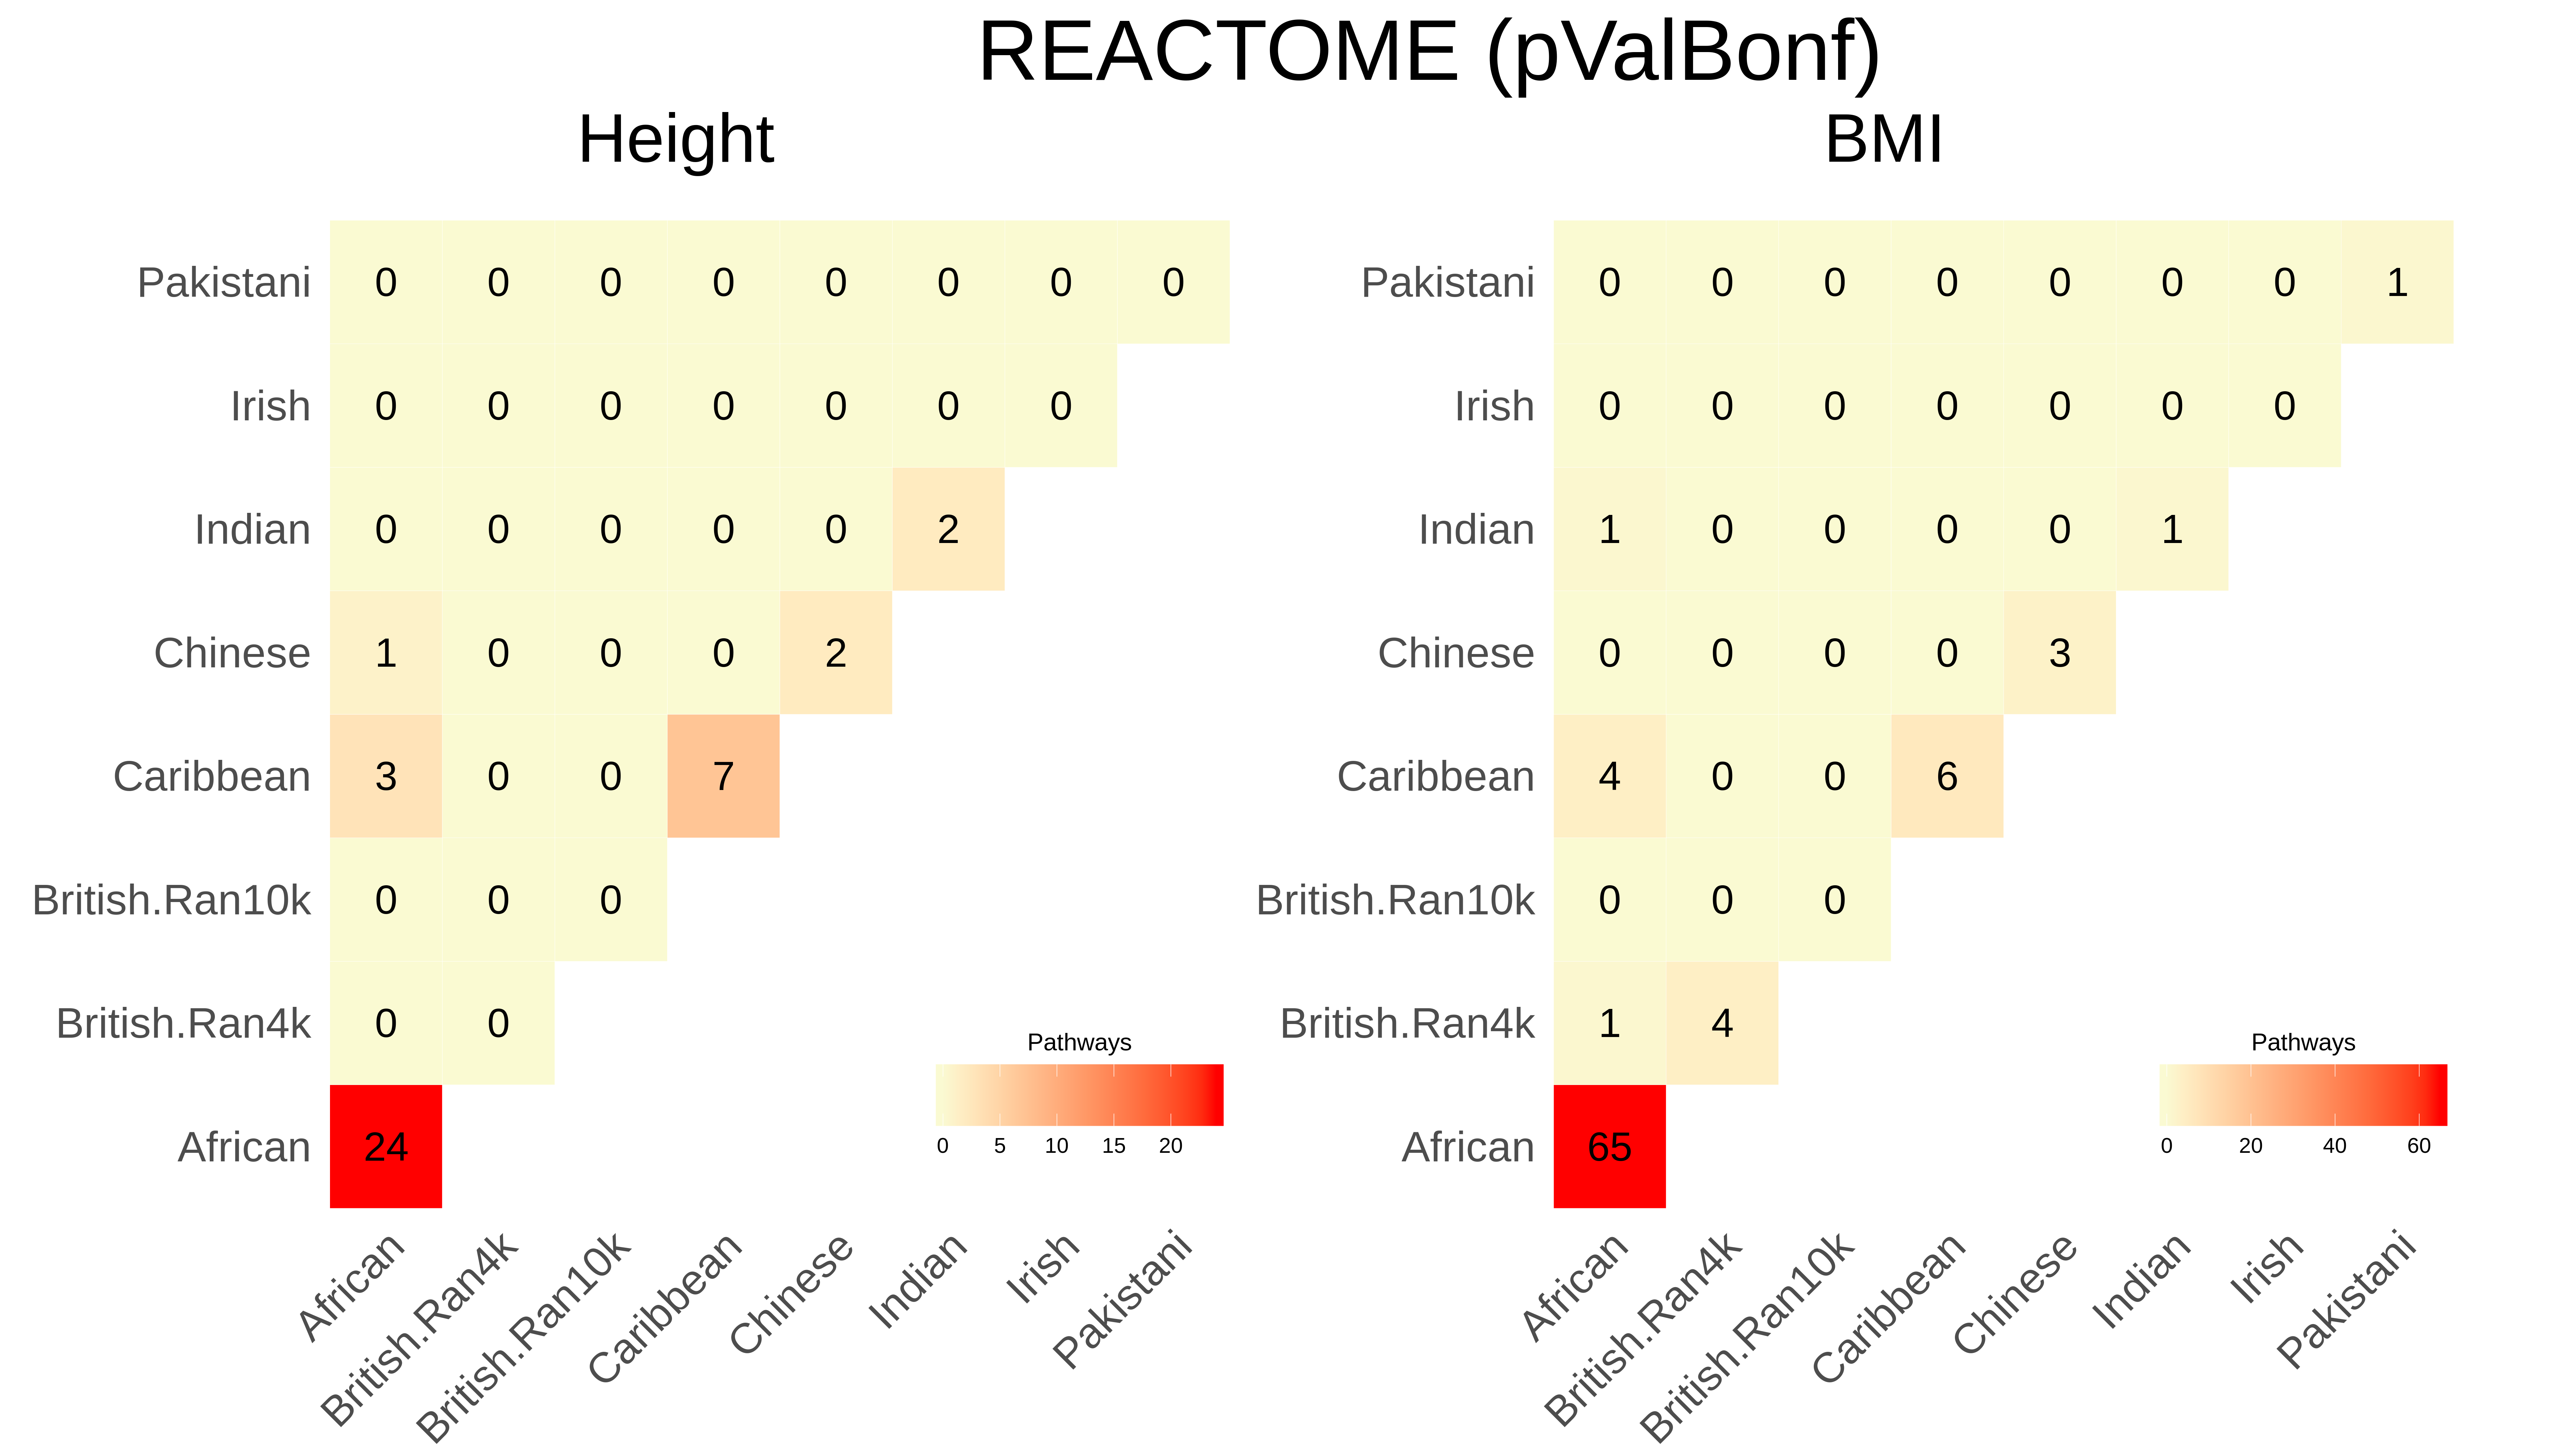
\includegraphics[scale=.225]{Images/Supp/InterPath_Supp_Figure_Heatplots_REACTOME_vs1.png}
%\caption[TBD]{\textbf{TBD}. \\ See above (this would be a supplementary figure).}
%\label{InterPath-Supp-Figure-Heatplots-REACTOME}
%\end{figure}
%\clearpage

\setlength{\footskip}{1cm}
\begin{figure}[htbp]
\centering
\vspace*{-2cm}
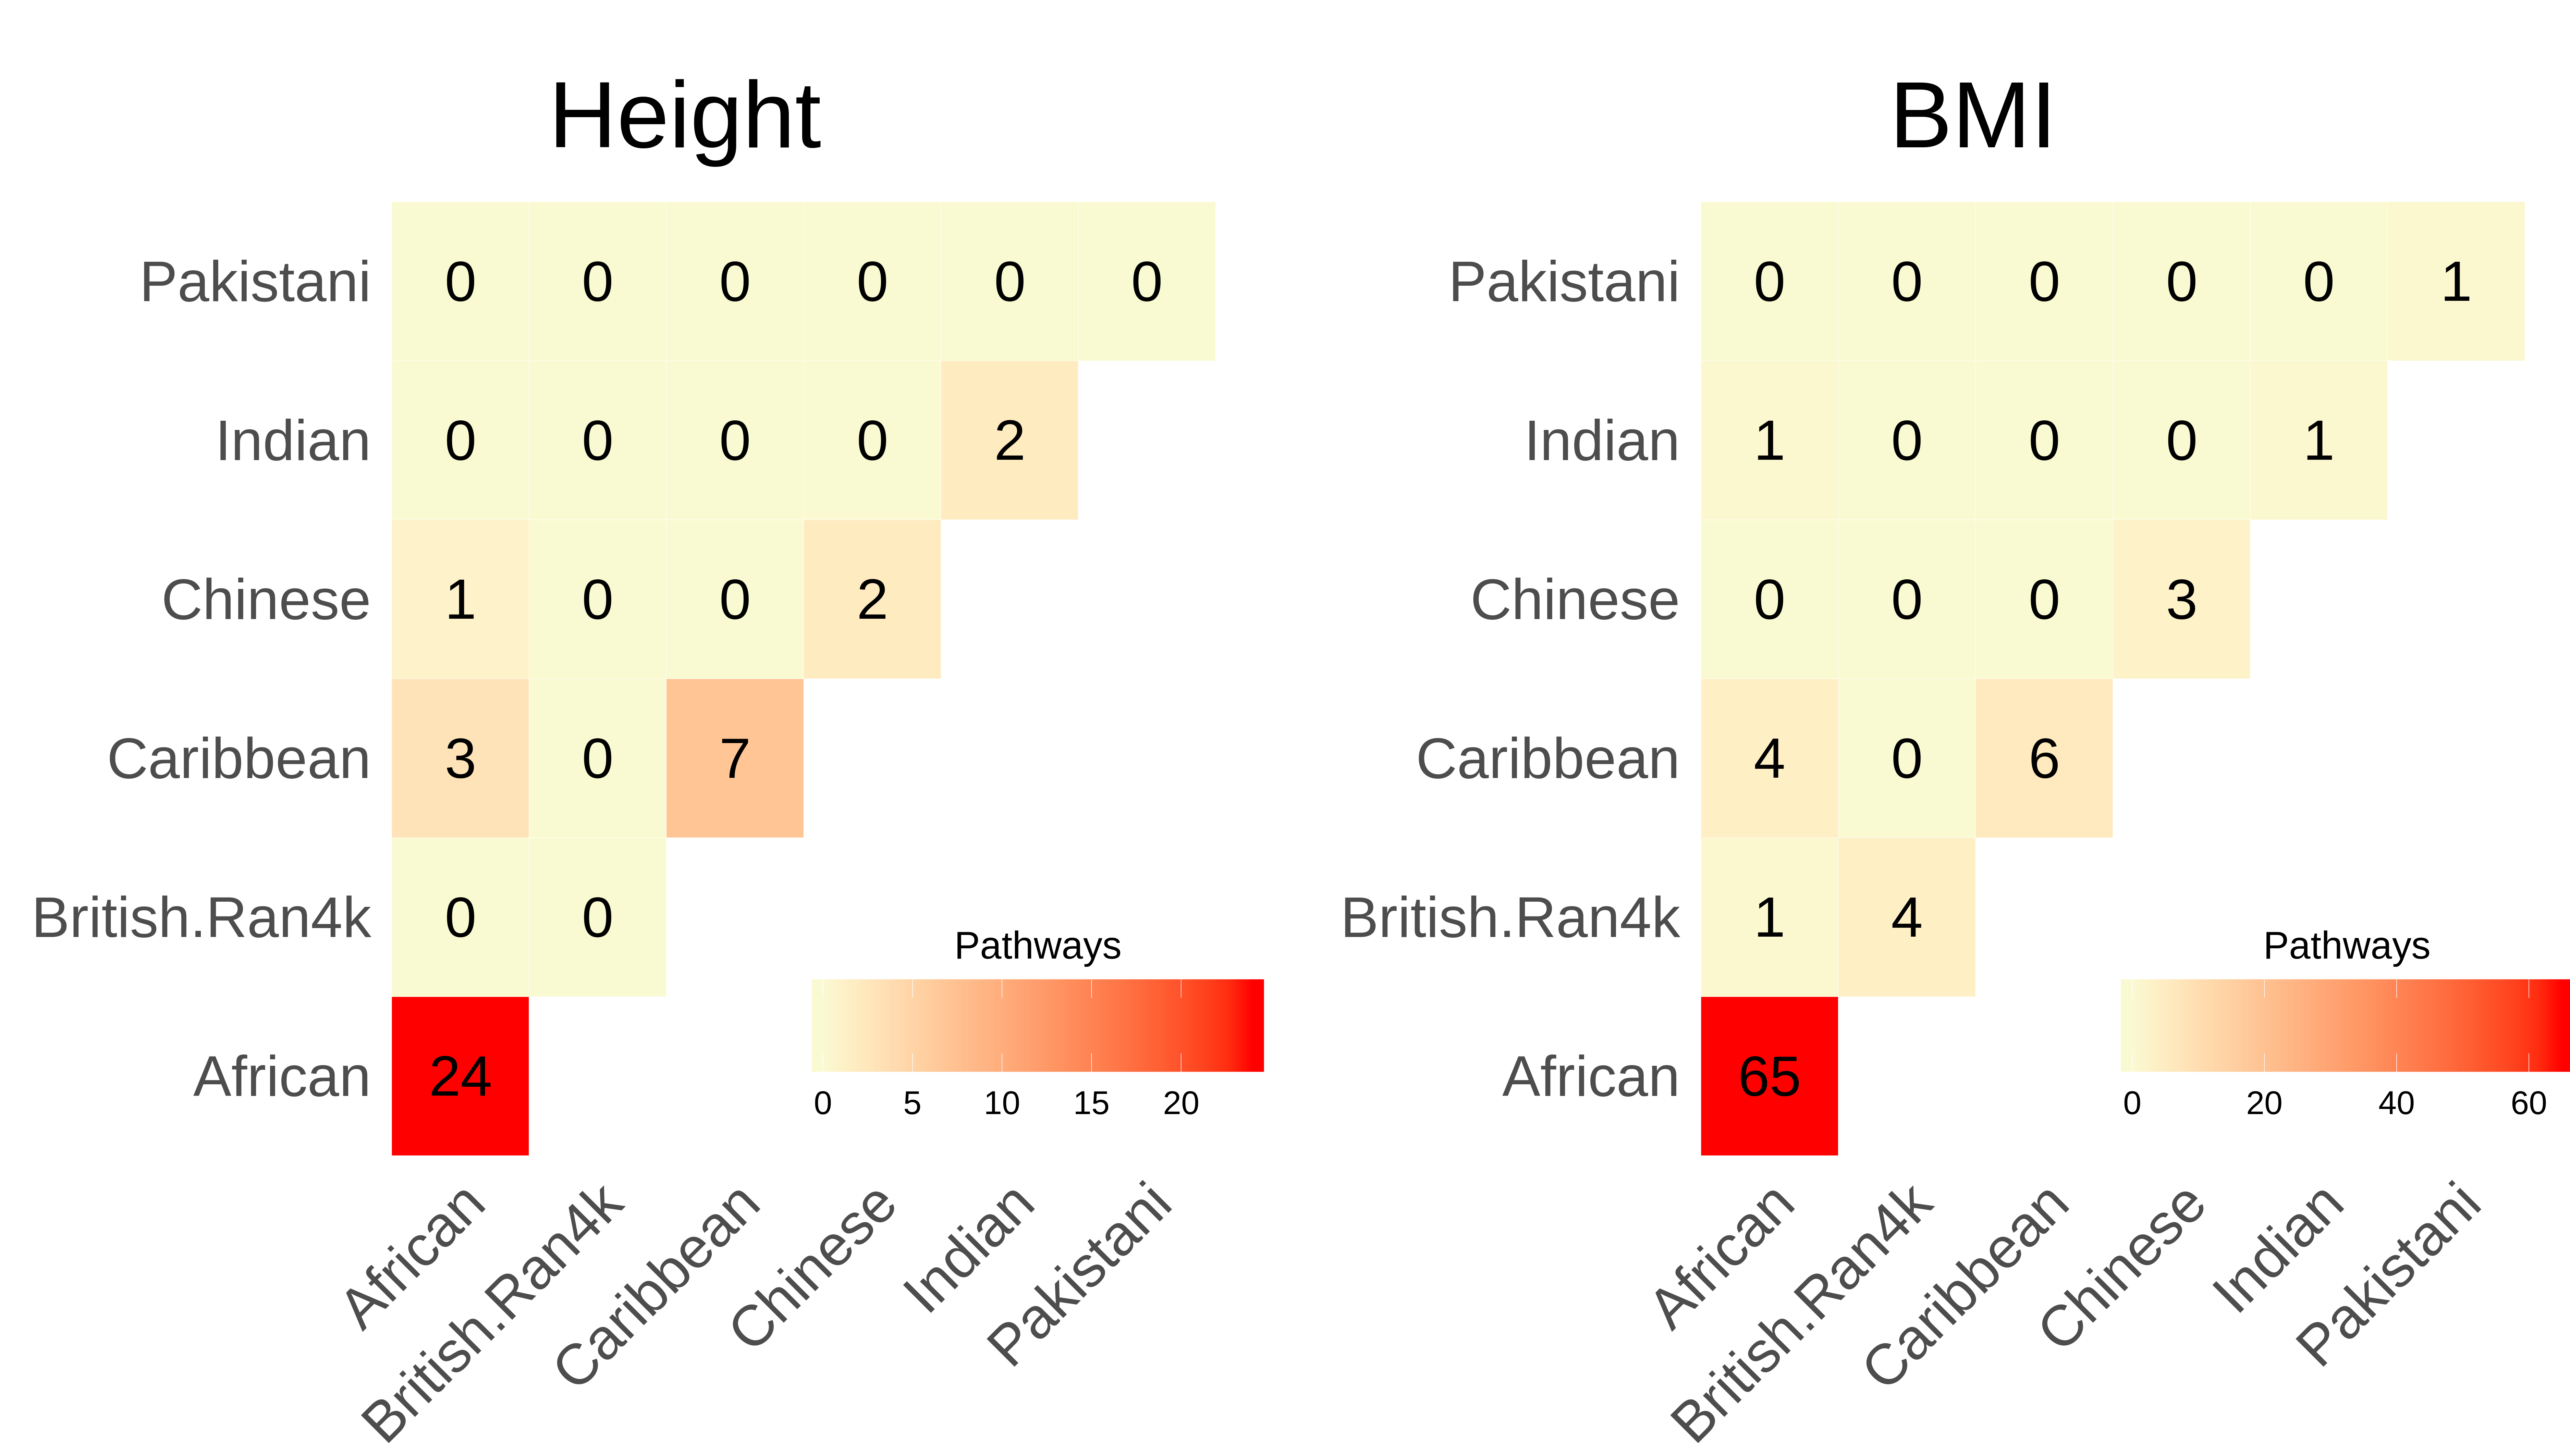
\includegraphics[scale=.225]{Images/Supp/InterPath_Supp_Figure_Heatplots_REACTOME_vs3.png}
\caption[TBD]{\textbf{Overlap of Genome-Wide Significant MAPIT-R Pathways Between UKB Population Subsets: REACTOME}. The heatplots show the numbers of genome-wide significant MAPIT-R pathways that overlap between each UKB subset for height and BMI in the REACTOME database. The diagonal shows the total number of genome-wide significant pathways per population subset. We observe that most subsets often have overlap with the African subset but rarely do so with the remaining non-African subsets. For results from the KEGG database see Figure \ref{InterPath-Main-Figure-Heatplots-KEGG}.}
\label{InterPath-Supp-Figure-Heatplots-REACTOME}
\end{figure}
\clearpage
\setlength{\footskip}{1cm}

%\begin{figure}[htbp]
%\centering
%\includegraphics[scale=.15]{Images/Main/InterPath_Main_PopCompDotPlots_African_vs1.png}
%\caption[]{\textbf{MAPIT-R Cross-Population KEGG $p$-value Comparisons: African}. Shown are comparisons of each population subset's MAPIT-R $p$-value for Height and BMI in KEGG against the African subset's MAPIT-R $p$-values. On the $x$-axis are the African subset's observed -$\log_{10}$ $p$-value and on the $y$-axis is the other population's observed -$\log_{10}$ $p$-value. Dotted red lines represent Bonferroni-corrected $p$-value thresholds for each population/phenotype combination.}
%\label{InterPath-Main-Figure-PopCompDotPlots}
%\end{figure}
%\clearpage

%\begin{figure}[htbp]
%\centering
%\includegraphics[scale=.15]{Images/Supp/InterPath_Supp_Figure_PhenoCompDotPlots_vs1.png}
%\caption[TBD]{\textbf{MAPIT-R Phenotype $p$-value Comparisons}. \\ Shown is a comparison of the MAPIT-R $p$-values for both phenotypes analyzed across all population subsets in the KEGG database. Shown on the $x$-axis is the observed height -$\log_{10}$ MAPIT-R $p$-value and shown on the $y$-axis is the observed BMI -$\log_{10}$ MAPIT-R $p$-value. Dotted red lines represent Bonferroni-corrected $p$-value thresholds for each population/phenotype combination (.05 / number of KEGG pathways analyzed). In general we observe a correlation between MAPIT-R $p$-values between each phenotype. In the African subset, where we have the most observed power, we find pathways that are significant in both phenotypes as well as each phenotype separately. Additionally, we observe, among marginally significant pathways, stronger MAPIT-R signals in BMI than height -- this is in line with previous observations that BMI may contain higher levels of epistasis than height (citations).}
%\label{InterPath-Supp-Figure-PhenoCompDotPlots}
%\end{figure}
%\clearpage

\setlength{\footskip}{3cm}
\begin{figure}[htbp]
\centering
\vspace*{-2cm}
\includegraphics[scale=.2]{Images/Supp/InterPath_Supp_Figure_MAPITR_PhenoComps_AllPops_vs2.png}
\caption[TBD]{\textbf{MAPIT-R Results: Height vs. BMI}. The figure shows MAPIT-R height results plotted against MAPIT-R BMI results for all pathways from the KEGG and REACTOME databases in all UKB subsets. The $x$-axes are the MAPIT-R height -$\log_{10}$ $p$-values and the $y$-axes are the MAPIT-R BMI -$\log_{10}$ $p$-values. The dotted red lines are the Bonferroni-corrected $p$-value thresholds for genome-wide significance in each subset, pathway, and phenotype combination.}
\label{InterPath-Supp-Figure-MAPITR-PhenoComps-AllPops}
\end{figure}
\clearpage
\setlength{\footskip}{1cm}

\begin{figure}[htbp]
\centering
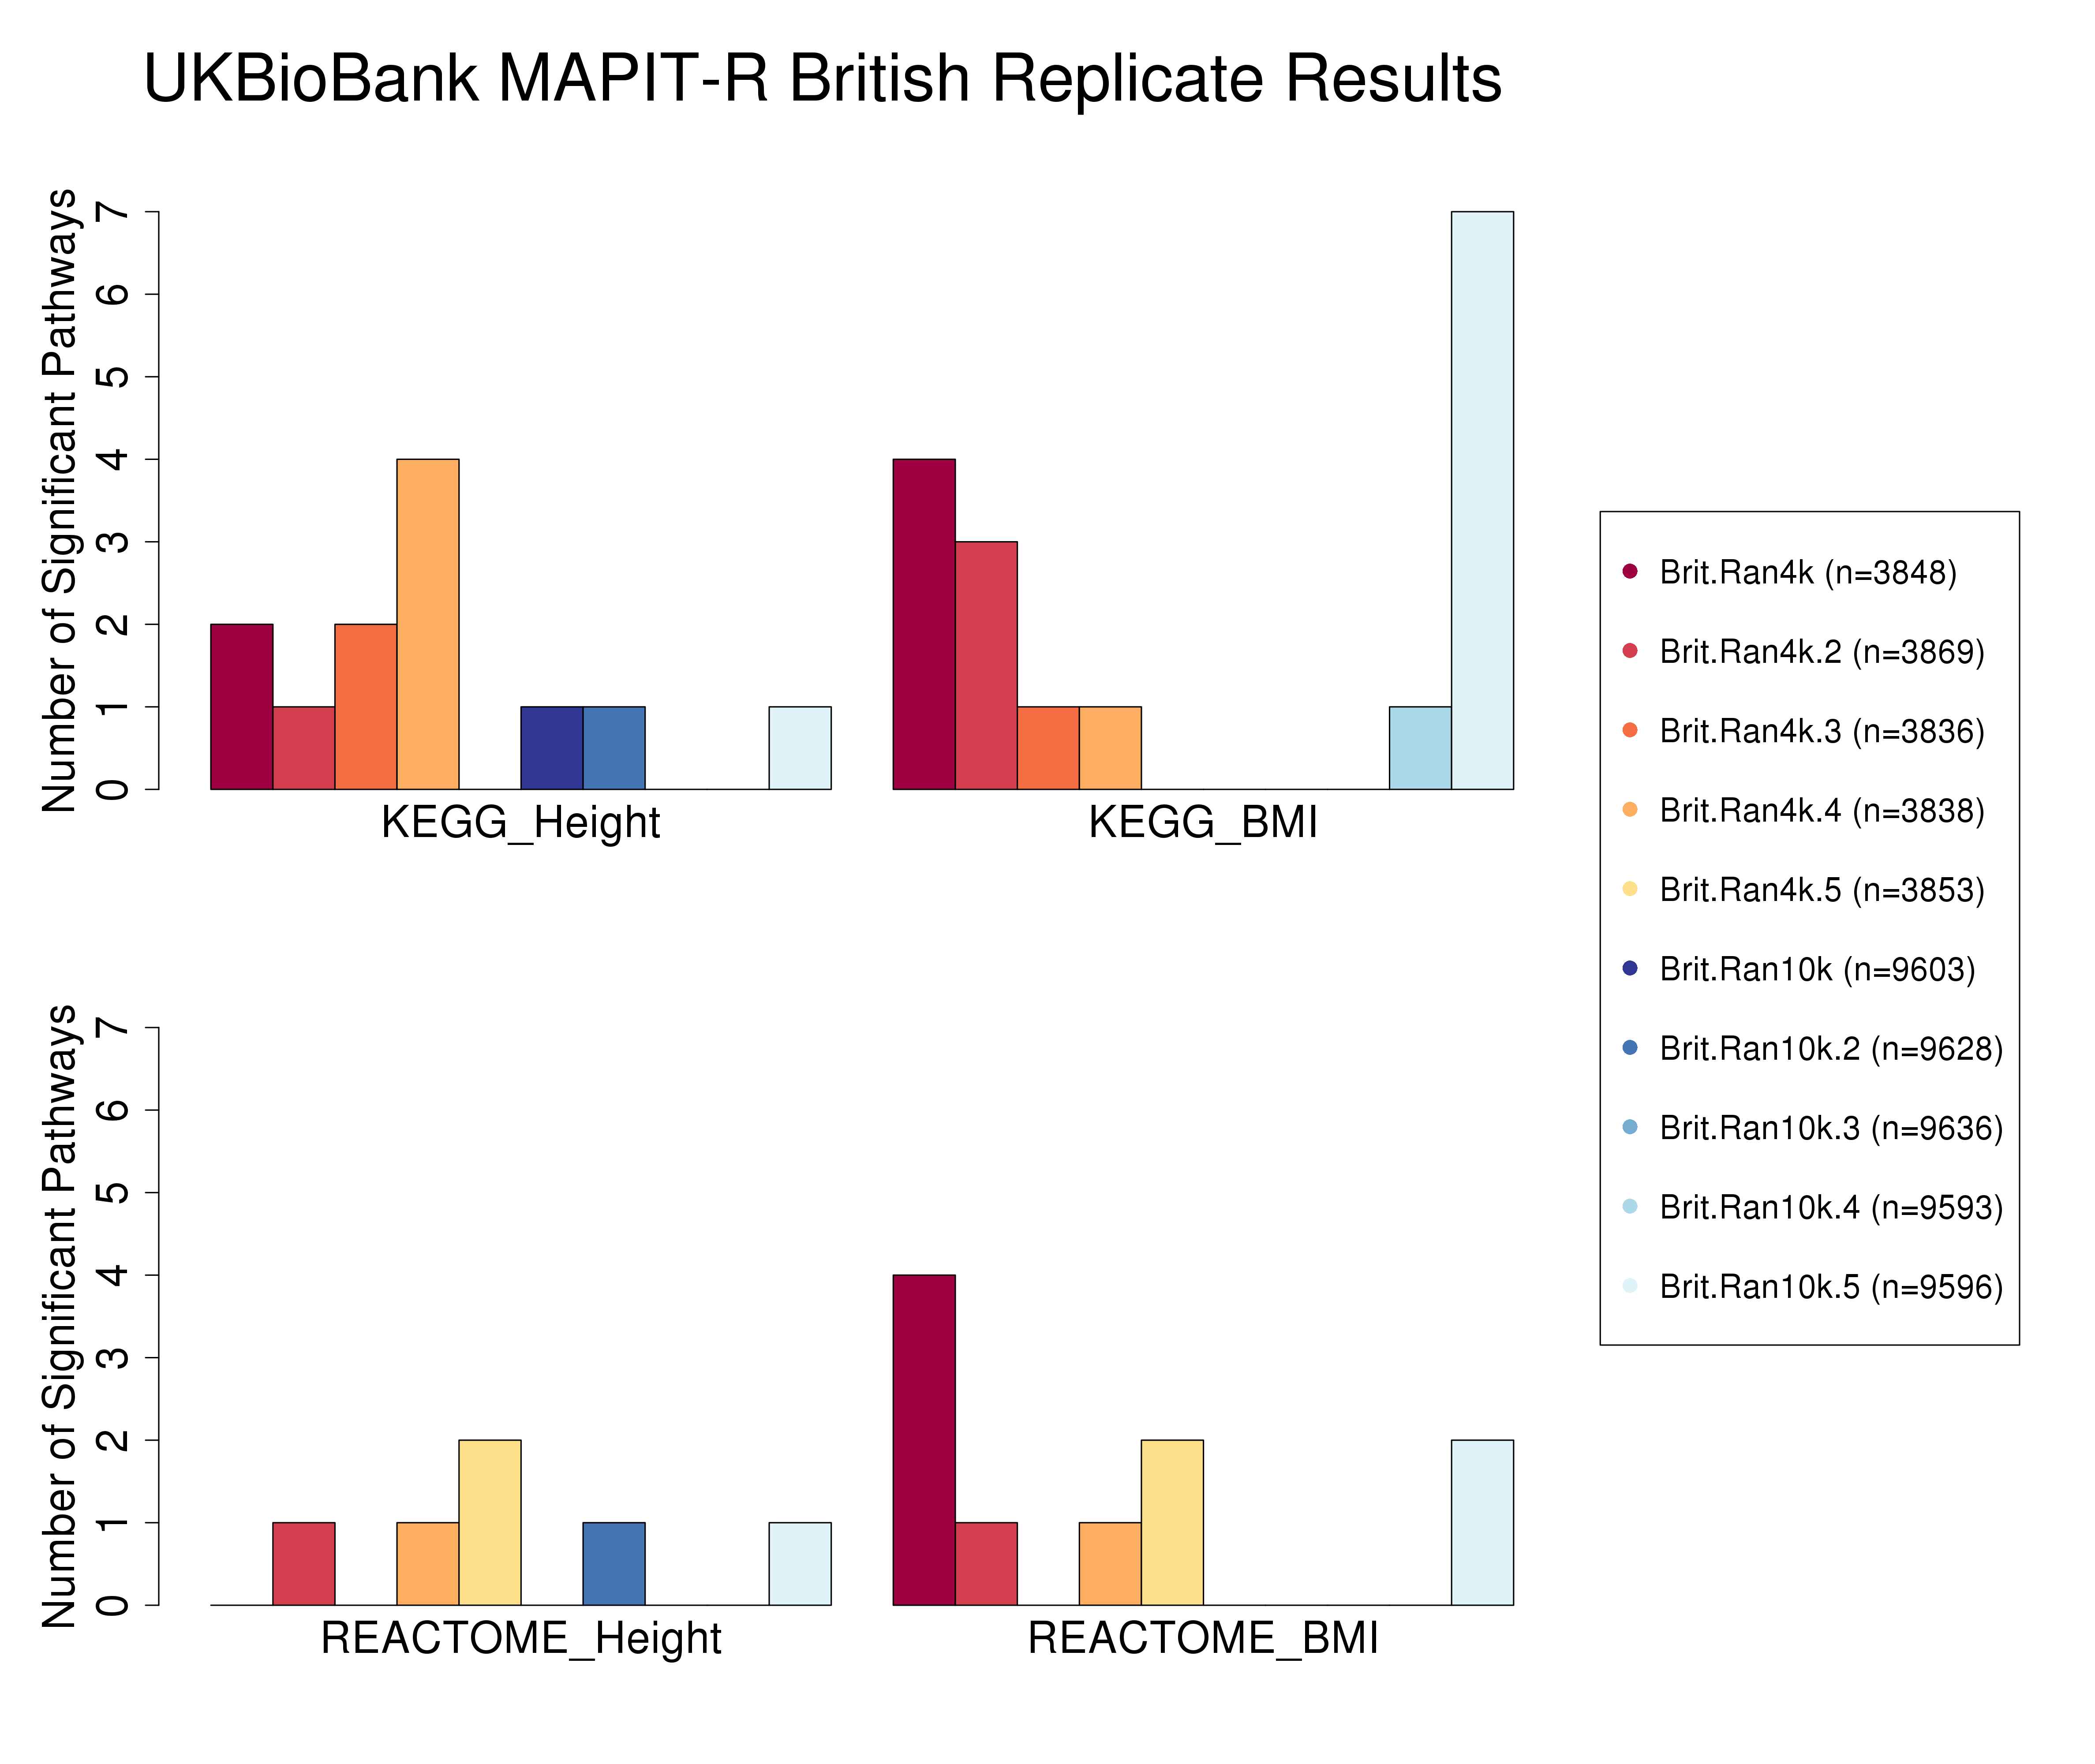
\includegraphics[scale=.45]{Images/Supp/InterPath_Supp_Figure_BritReps_Barplot_vs2.png}
\caption[TBD]{\textbf{MAPIT-R Results: British Replicates Barplots}. The barplots show the number of genome-wide significant pathways found from running MAPIT-R for both height and BMI in the KEGG and REACTOME databases on each of our British subsample replicate populations. Genome-wide significance was determined by using Bonferroni-corrected $p$-value thresholds based on the number of pathways tested in each phenotype, replicate, and pathway database combination. Most replicate runs did not produce many significant results.}
\label{InterPath-Supp-Figure-BritReps-Barplots}
\end{figure}
\clearpage

\setlength{\footskip}{2cm}
\begin{figure}[htbp]
\centering
\hspace*{-1.5cm}
%\vspace*{-2cm}
\includegraphics[scale=.24]{Images/Supp/InterPath_Supp_Figure_BritReps_Heatplots_AllPaths_vs2.png}
\caption[TBD]{\textbf{Overlap of Genome-Wide Significant MAPIT-R Pathways Between British Replicates Subsets}. The heatplots show the numbers of genome-wide significant MAPIT-R pathways that overlap between each British replicate subset for height and BMI in the KEGG and REACTOME databases. The diagonal shows the total number of genome-wide significant pathways per population subset.}
\label{InterPath-Supp-Figure-BritReps-Heatplots-AllPaths}
\end{figure}
\clearpage
\setlength{\footskip}{1cm}

\begin{figure}[htbp]
\centering
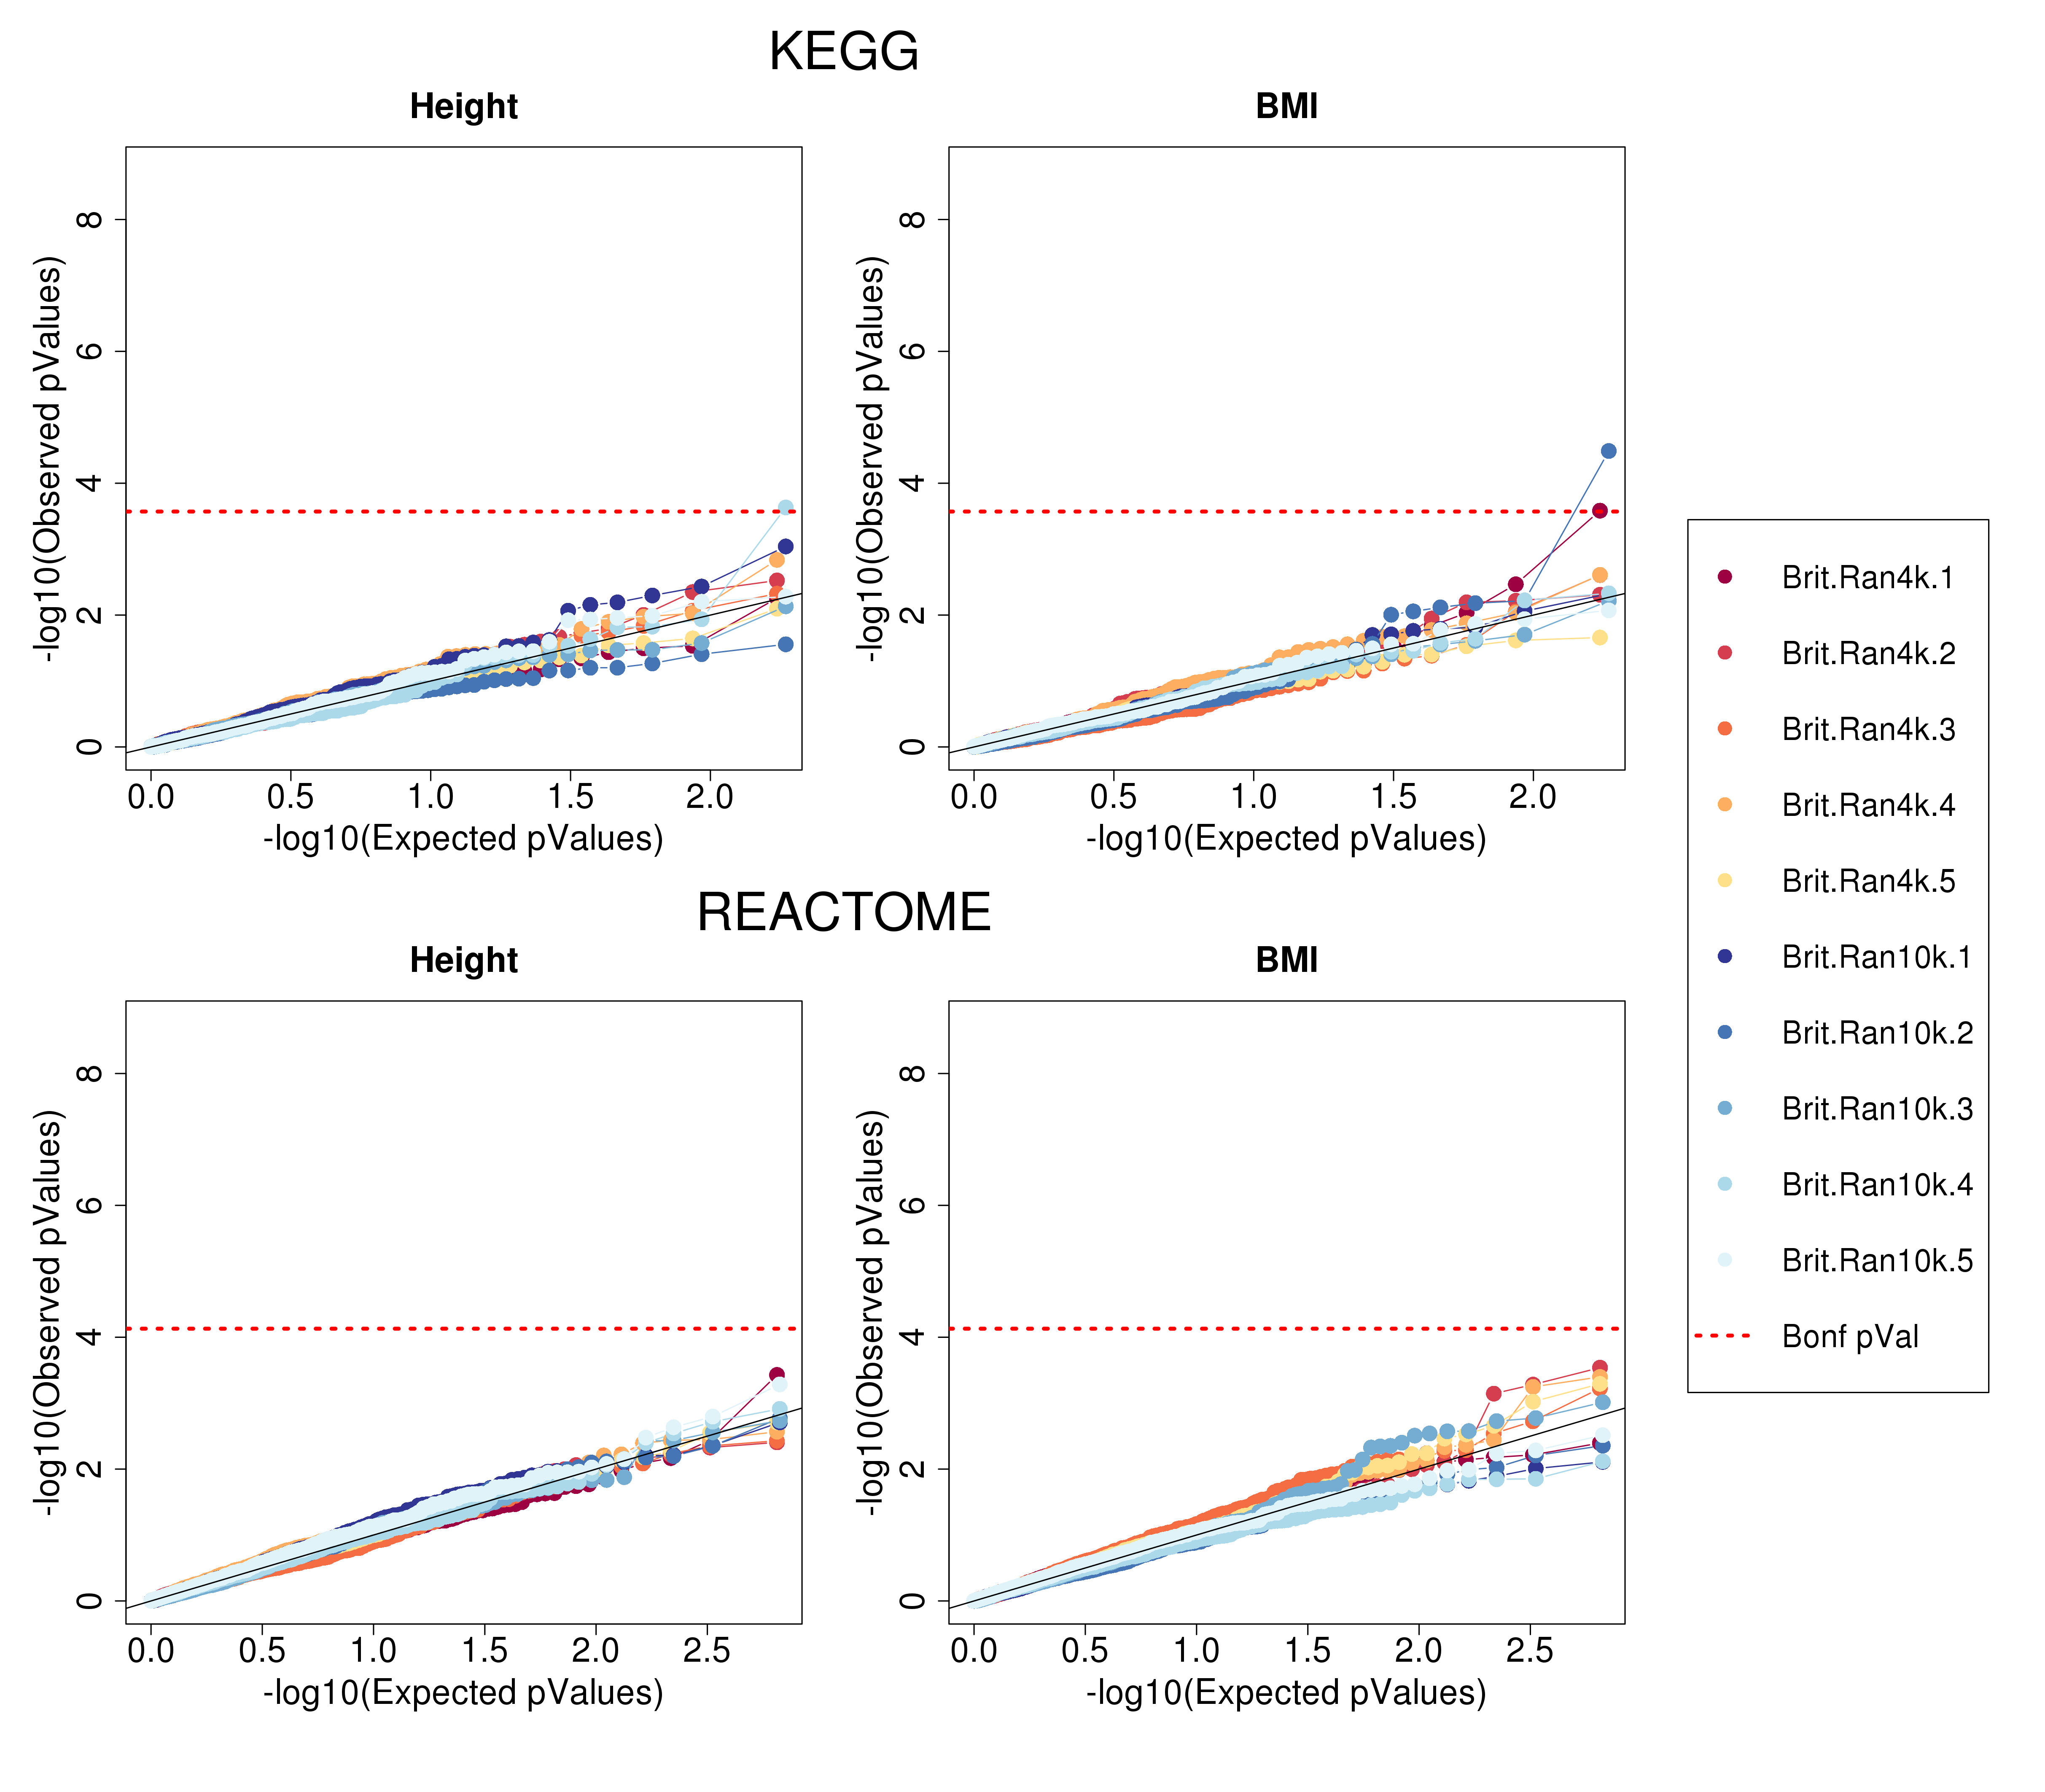
\includegraphics[scale=.35]{Images/Supp/InterPath_Supp_Figure_BritReps_perm1_QQPlots_AllPaths_vs1.png}
\caption[TBD]{\textbf{MAPIT-R Results: British Replicates Phenotype Permutation QQ-Plots}. The figure shows QQ-plots for running MAPIT-R using single, permuted versions of both height and BMI with the KEGG \& REACTOME databases. Phenotypes were permuted within each British replicate subset. Shown on the $x$-axis are the -$\log_{10}$ of our expected $p$-values and the on the $y$-axis are on the -$\log_{10}$ of our observed $p$-values. The dotted red line is our Bonferroni-corrected $p$-value threshold based on the number of pathways tested per phenotype and pathway database combination. We find across all replicate, phenotype, and pathway database combinations that MAPIT-R continues to show proper null behavior within the range expected when using permuted phenotypes.}
\label{InterPath-Supp-Figure-BritReps-perm1-QQPlots-AllPaths}
\end{figure}
\clearpage

\newcounter{CharNumber3}
\setcounter{CharNumber3}{1}
\renewcommand{\thefigure}{\arabic{figure}\alph{CharNumber3}}
\setlength{\footskip}{1cm}
\begin{figure}[htbp]
\centering
\vspace*{-1cm}
\includegraphics[scale=.2]{Images/Supp/InterPath_Supp_Figure_BritReps_pValHists_AllPaths_vs1_pt1.png}
\caption[TBD]{\textbf{MAPIT-R Results: British Replicates Permutation $p$-Value Histograms (Ran4k Subsets)}. The figure shows histograms of MAPIT-R $p$-values collected across ten independent phenotype permutation runs for each British subsample replicate. The same phenotype permutation for a given replicate was used across both pathway databases (i.e. 10 permutations were done for height and 10 done for BMI for each subset). Covariates used from the original MAPIT-R analysis were kept the same.}
\label{InterPath-Supp-Figure-BritReps-10perms-pValHists-pt1}
\end{figure}
\clearpage
\setlength{\footskip}{1cm}
\addtocounter{figure}{-1}
\addtocounter{CharNumber3}{1}

\setlength{\footskip}{2cm}
\begin{figure}[htbp]
\centering
\vspace*{-1cm}
\includegraphics[scale=.2]{Images/Supp/InterPath_Supp_Figure_BritReps_pValHists_AllPaths_vs1_pt2.png}
\caption[TBD]{\textbf{MAPIT-R Results: British Replicates Permutation $p$-Value Histograms (Ran10k Subsets)}. See Supplementary Figure \ref{InterPath-Supp-Figure-BritReps-10perms-pValHists-pt1}.}
\label{InterPath-Supp-Figure-BritReps-10perms-pValHists-pt2}
\end{figure}
\clearpage
\setlength{\footskip}{1cm}
\renewcommand{\thefigure}{\arabic{figure}}

\begin{figure}[htbp]
\centering
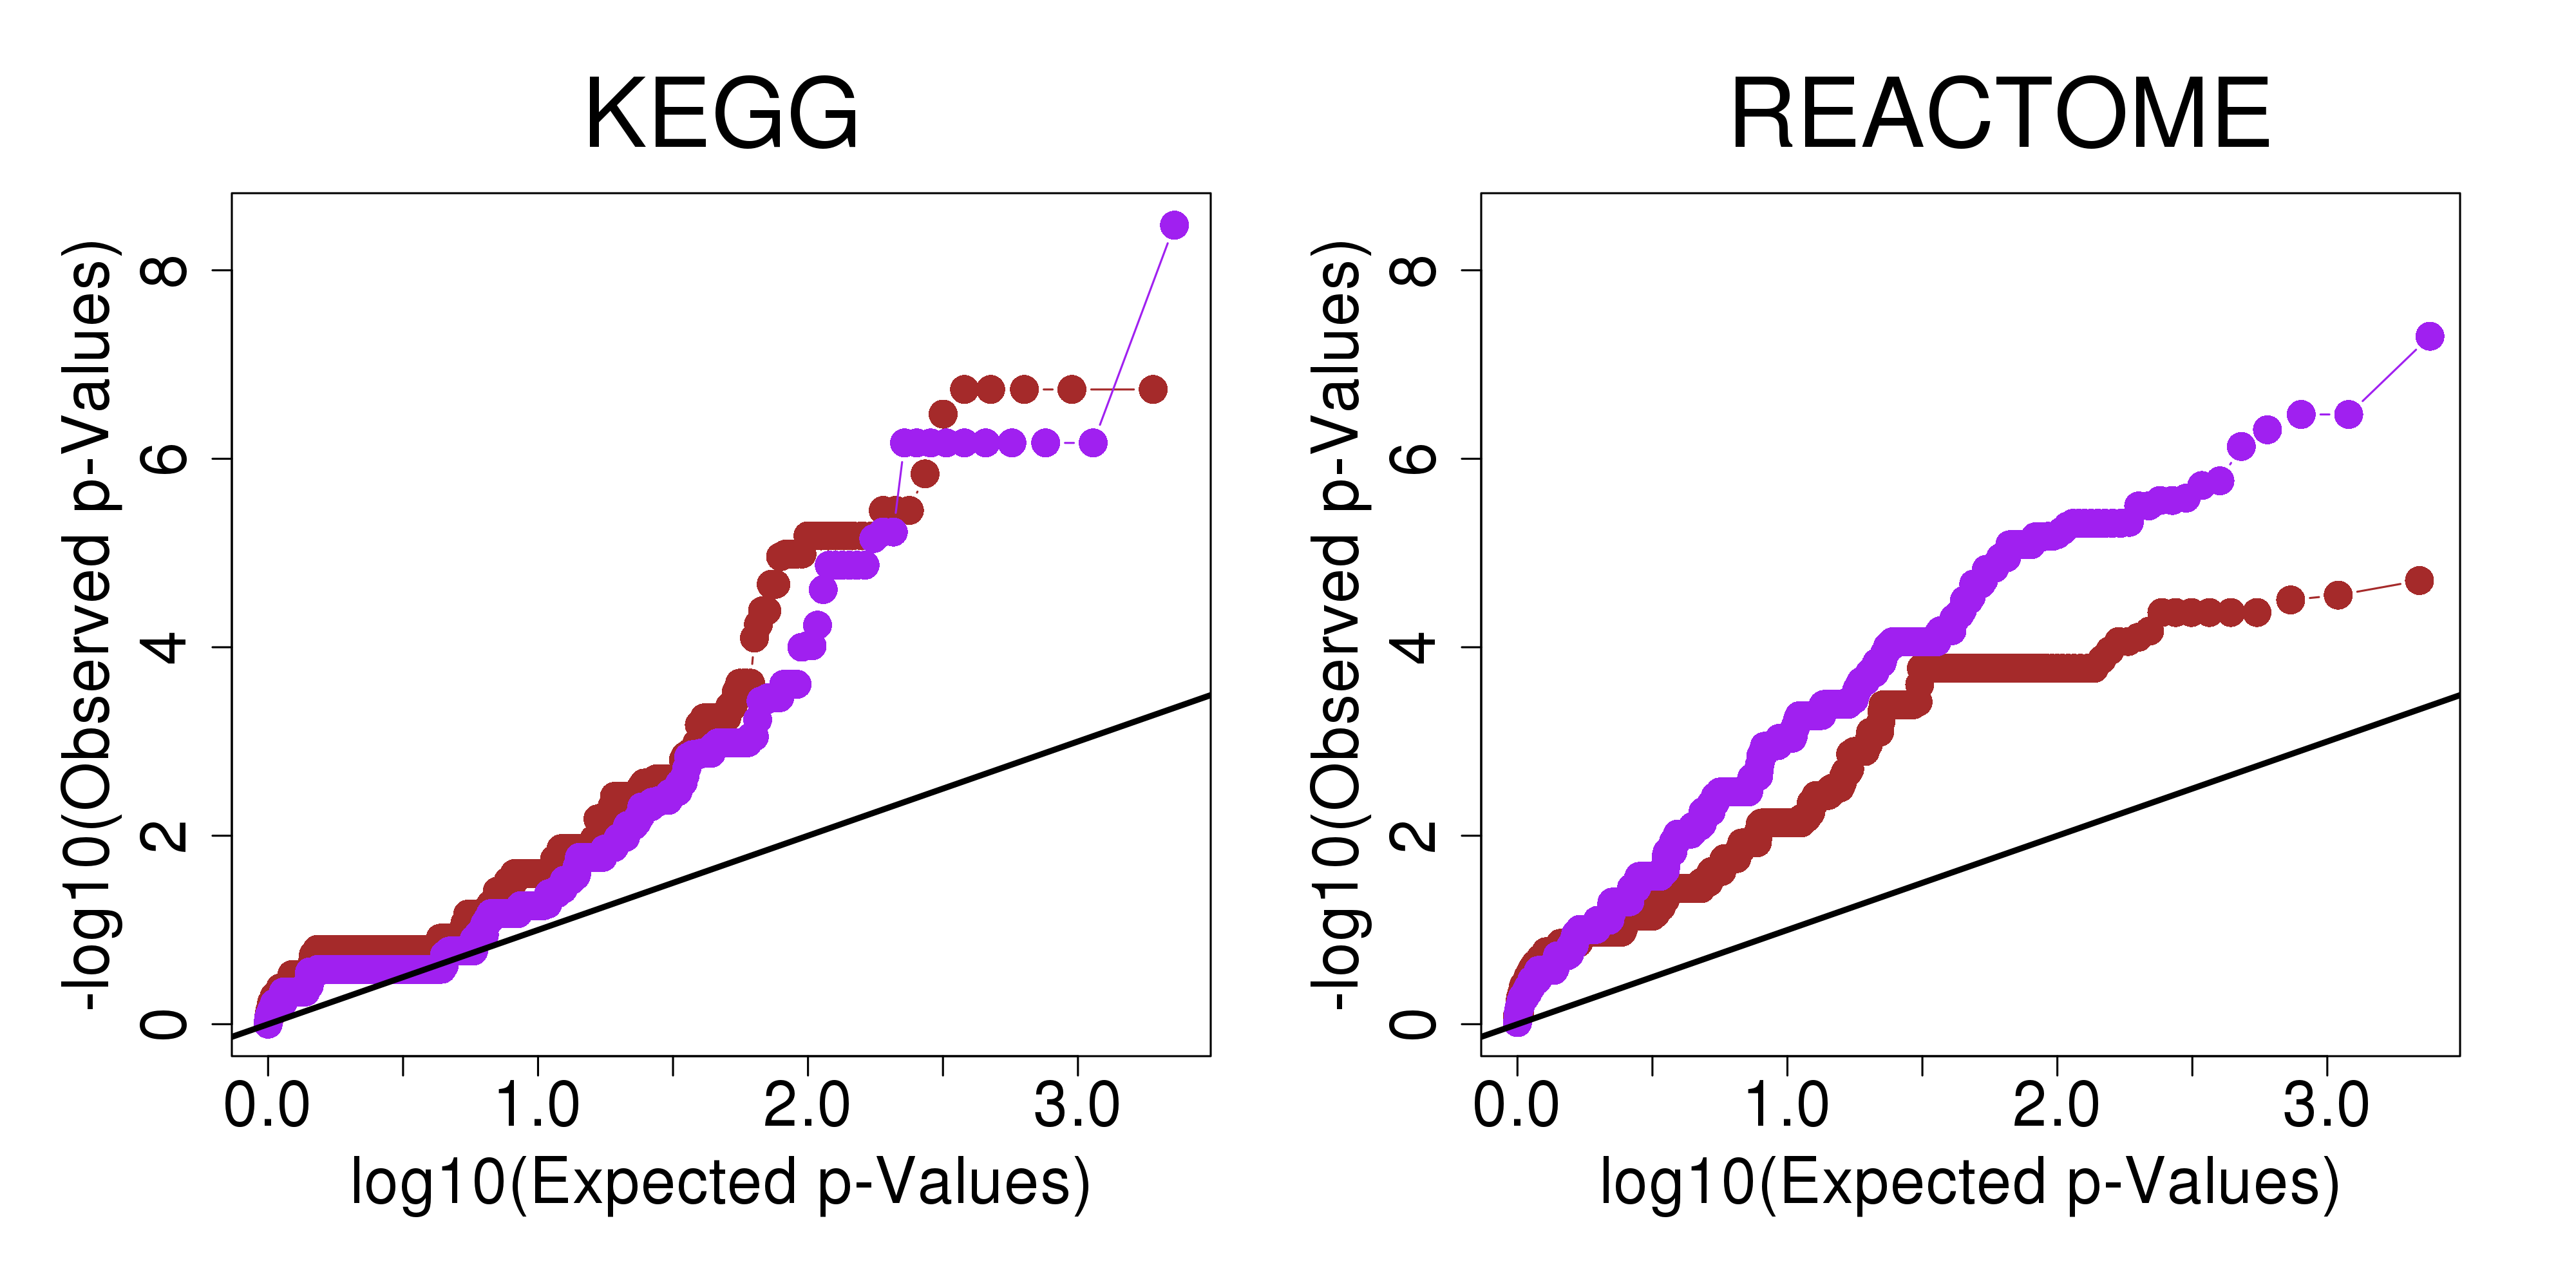
\includegraphics[scale=.45]{Images/Supp/InterPath_Supp_Figure_Hypergeometric_QQPlots_African_vs1.png}
\caption[TBD]{\textbf{Gene Count Hypergeometric Enrichment Tests: African QQ-Plots}. The figure shows QQ-plots of the gene count hypergeometric enrichment results for the African subset in both height and BMI and across both the KEGG and REACTOME databases. Every gene that was present among the set of MAPIT-R genome-wide significant pathways for that phenotype and pathway database combination was tested, including genes that were only present once. The $x$-axis is the expected -$\log_{10}$ $p$-values and the $y$-axis is the observed -$\log_{10}$ $p$-values. Brown dots are results from the height analysis and purple dots are results from the BMI analysis.}
\label{InterPath-Supp-Figure-Hypergeometric-QQPlots-African}
\end{figure}
\clearpage

\begin{figure}[htbp]
\centering
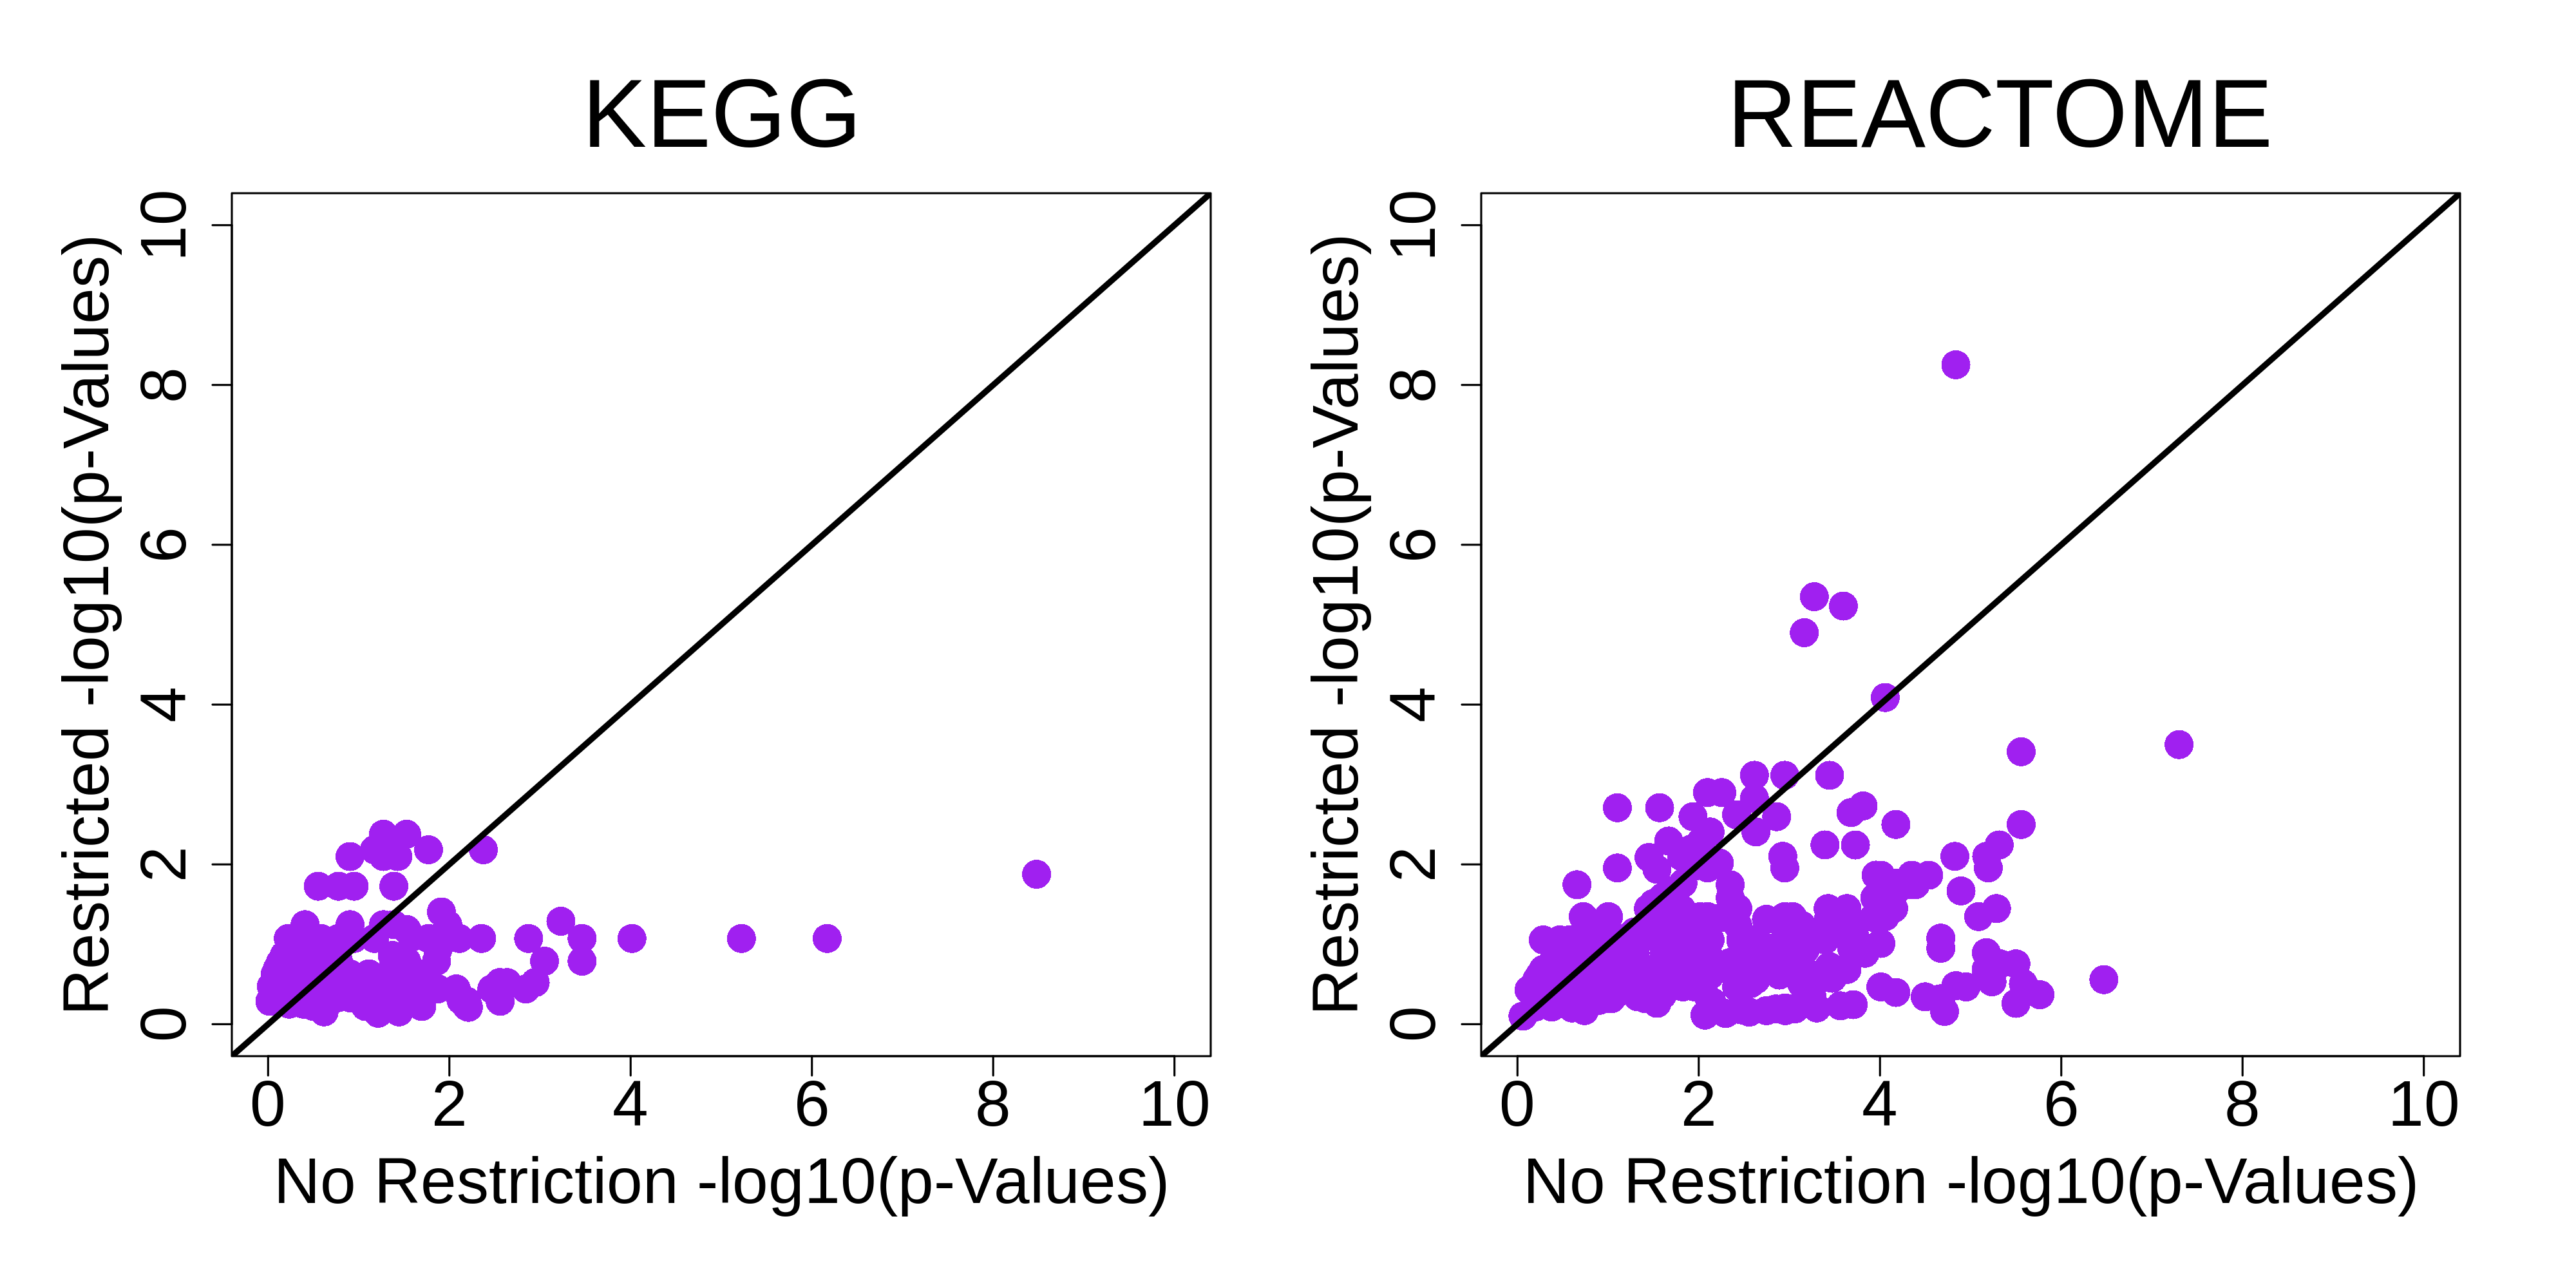
\includegraphics[scale=.45]{Images/Supp/InterPath_Supp_Figure_Hypergeometric_RestrictedComps_African_BMI_vs1.png}
\caption[TBD]{\textbf{Gene Count Hypergeometric Enrichment Tests: African BMI Size Restriction $p$-Value Comparisons}. The figure shows comparisons of the gene count hypergeometric enrichment $p$-values between the size restricted version of the analysis and the original unrestricted version of the analysis. The size restricted version of the analysis is redoing the hypergeometric enrichment tests but only using pathways that contained $<=$ 1,000 SNPs. Only results for BMI are shown here since almost all Bonferroni significant pathways were lost in the height results due to this size restriction step. The $x$-axis shows the original, unrestricted hypergeometric -$\log_{10}$ $p$-values, and the $y$-axis shows the new, size restricted hypergeoemtric -$\log_{10}$ $p$-values. The PSM* gene cluster is highlighted in the REACTOME plot. For lists of the top genes that became more significant due to the size restriction step, see Supplementary Table \ref{InterPath-Supp-Table-Hypergeometric-RestrictedComps-African-BMI-TopExamples}.}
\label{InterPath-Supp-Figure-Hypergeometric-RestrictedComps-African-BMI}
\end{figure}
\clearpage

\setlength{\footskip}{3cm}
\begin{figure}[htbp]
\centering
\vspace*{-2cm}
\includegraphics[scale=.15]{Images/Supp/InterPath_Supp_Figure_IBS_AllPops_vs2.png}
\caption[TBD]{\textbf{Mean Pairwise IBS Proportions vs. MAPIT-R $p$-values in All Subset, Phenotype, and Database Combinations}. The figure shows the mean pairwise IBS proportions per pathway plotted against each pathway's MAPIT-R $p$-value for every UKB subset, phenotype, and pathway database combination. IBS proportions were calculated per pathway by using that pathway's set of SNPs, were calculated pairwise between every set of individuals in the subset, and then averaged across each of these pairs for a final, single summary metric. We observe across almost every combination no significant relationship between mean pairwise IBS proportion and MAPIT-R $p$-value.}
\label{InterPath-Supp-Figure-IBS-AllPops}
\end{figure}
\clearpage
\setlength{\footskip}{1cm}

\begin{figure}[htbp]
\centering
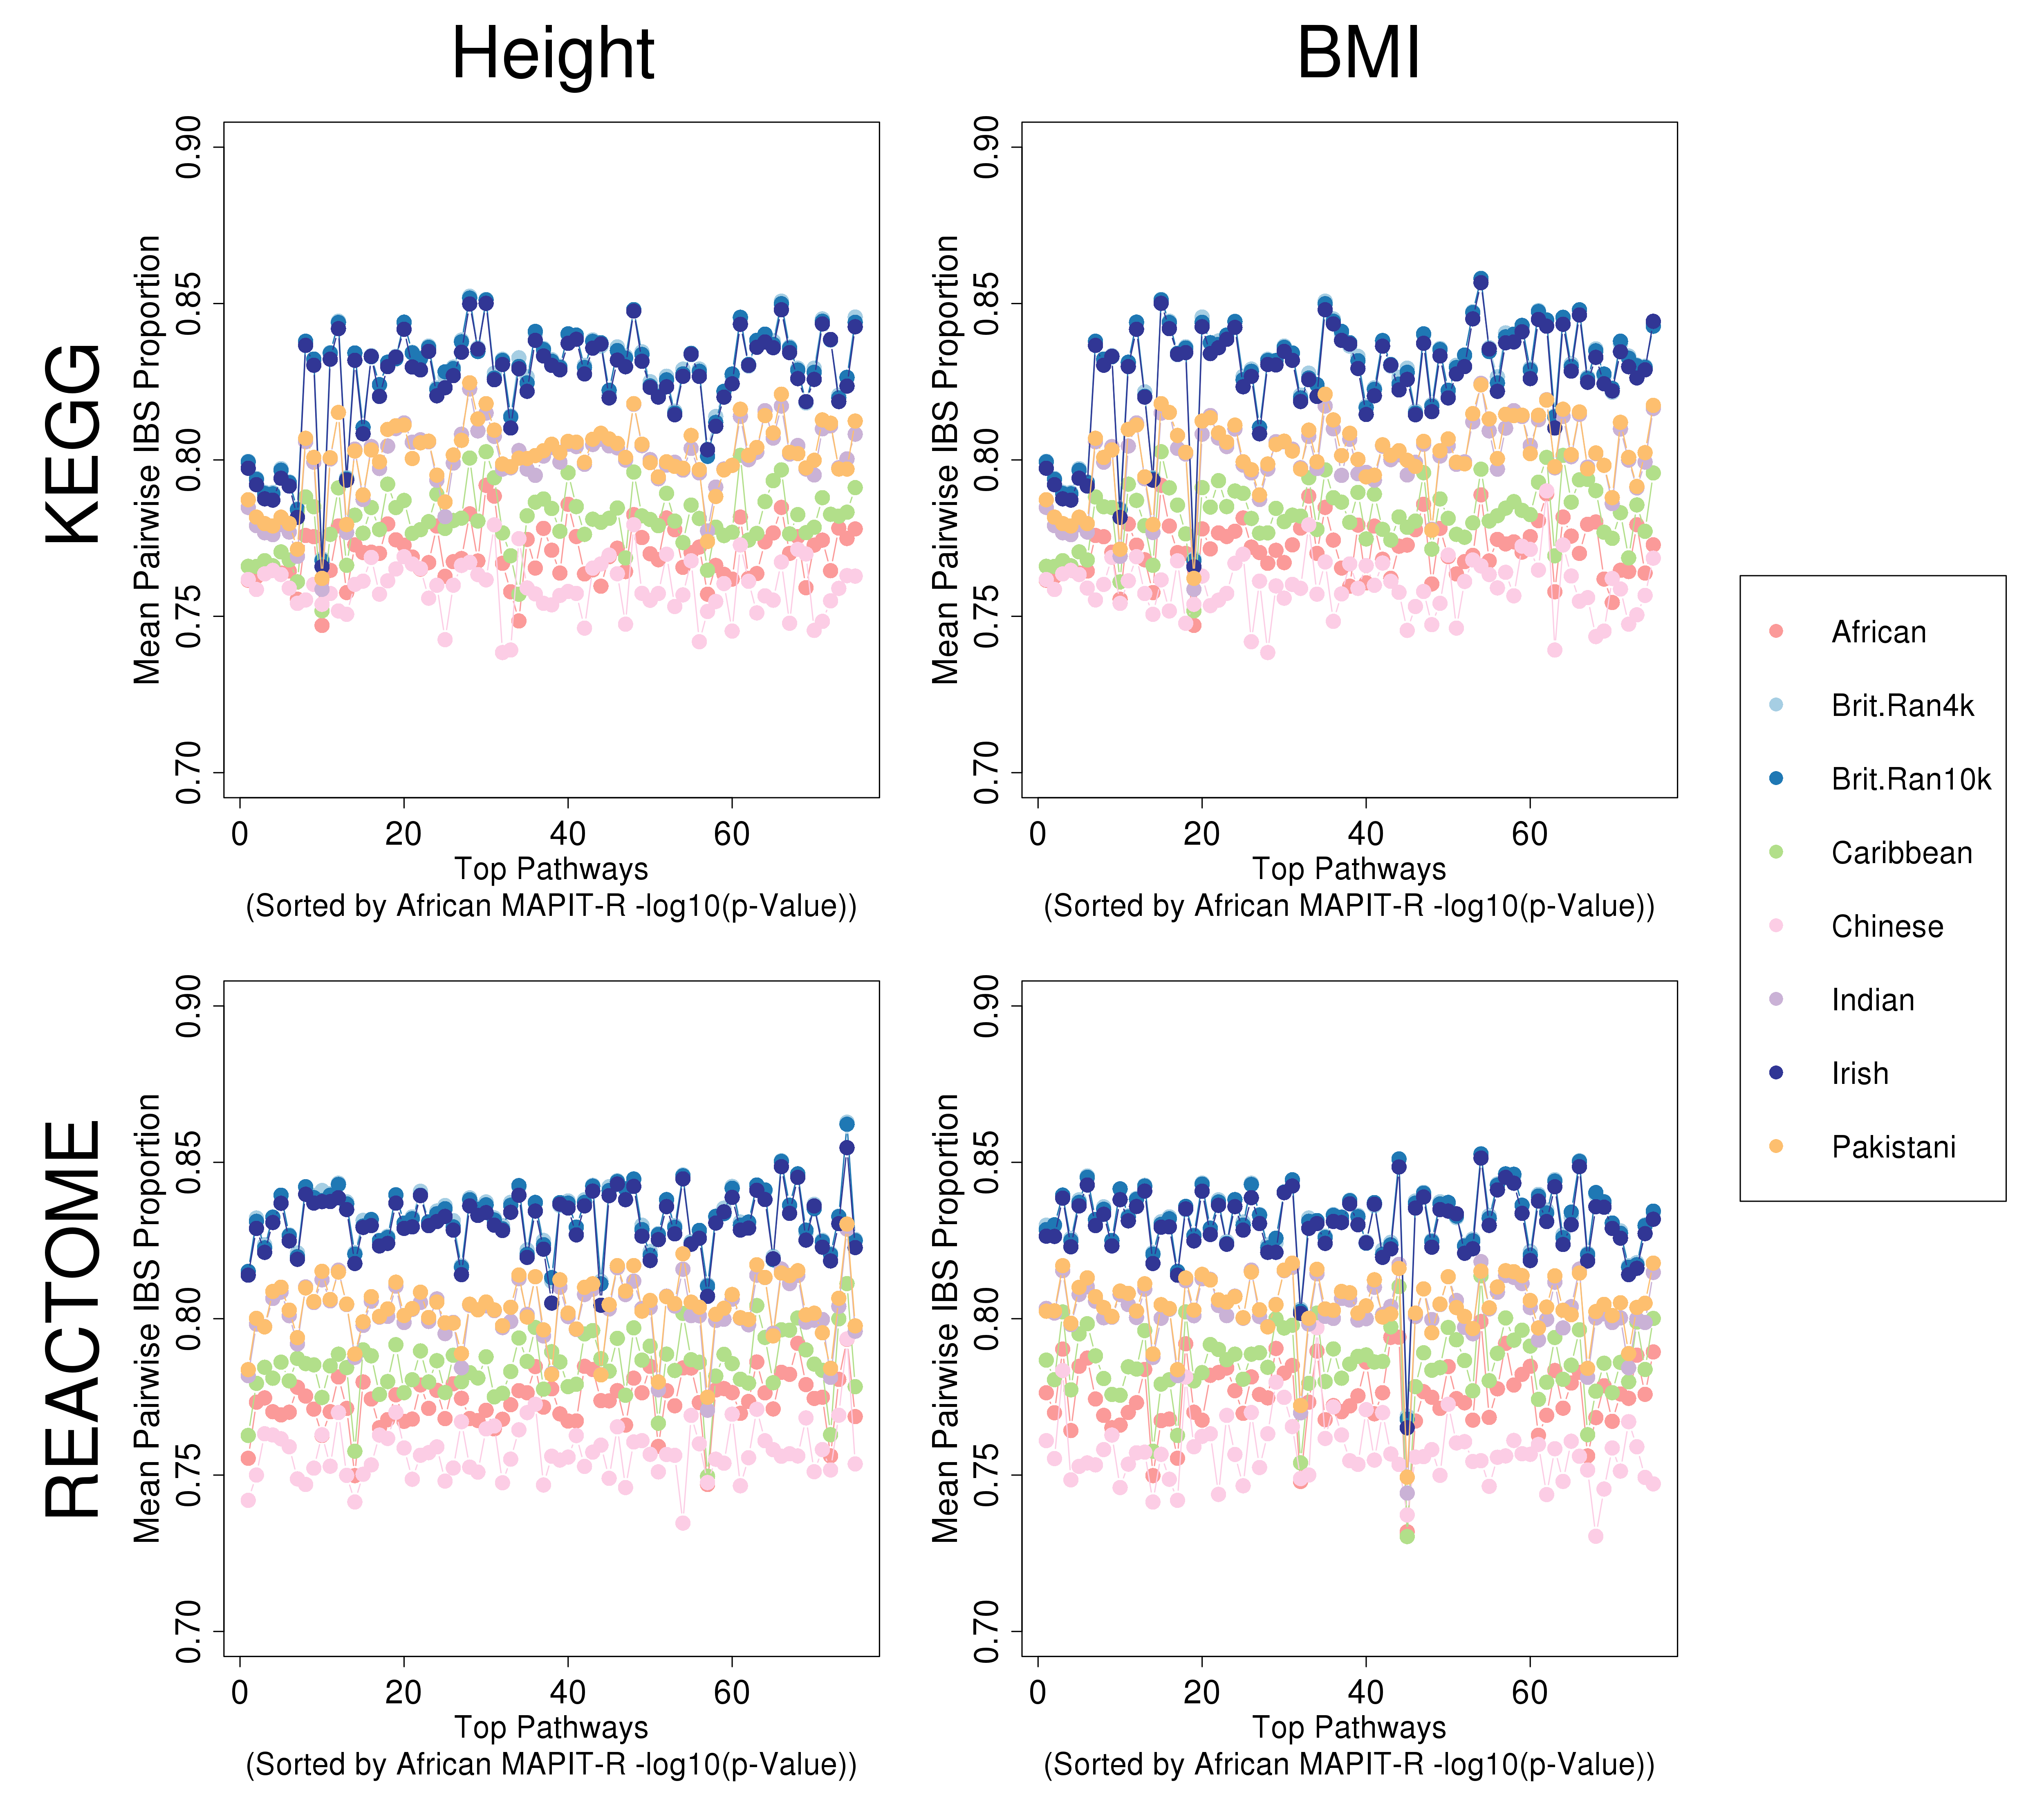
\includegraphics[scale=.35]{Images/Supp/InterPath_Supp_Figure_IBS_AllPopComps_vs2.png}
\caption[TBD]{\textbf{Mean Pairwise IBS Proportions Across Each Subset in Top African Pathways}. The figure plots the mean pairwise IBS proportions of each UKB subset for the top 75 African pathways (sorted by MAPIT-R $p$-value) for each phenotype and pathway database combination. Most variation in mean pairwise IBS proportions varies moreso based on the pathways themselves and not on ancestry; subsets differ between one another mostly at the same levels across each pathway.}
\label{InterPath-Supp-Figure-IBS-AllPopComps}
\end{figure}
\clearpage

\section{Supplementary Tables}\label{Supplementary-Tables}

\begin{table}[ht]
\centering
\begin{tabular}{ccccc}
  \hline
\textbf{UK BioBank} & \textbf{Individuals} & \textbf{SNPs} & \textbf{KEGG} & \textbf{REACTOME} \\
\textbf{Subset} & & & \textbf{Pathways} & \textbf{Pathways}  \\
  \hline
\textbf{Original Subsets:} & & & & \\
African & 3111 & 374466 & 180 & 658 \\ 
British.Ran4000 & 3848 & 600006 & 173 & 650 \\ 
Caribbean & 3833 & 410017 & 181 & 661 \\ 
Chinese & 1448 & 345221 & 153 & 626 \\ 
Indian & 5077 & 505854 & 181 & 662 \\ 
Pakistani & 1581 & 516806 & 141 & 596 \\ 
\\
\textbf{British Replicates:} & & & & \\
British.Ran4000.2 & 3869 & 599381 & 173 & 650 \\ 
British.Ran4000.3 & 3836 & 600654 & 173 & 649 \\ 
British.Ran4000.4 & 3838 & 599829 & 173 & 650 \\ 
British.Ran4000.5 & 3853 & 599442 & 173 & 650 \\ 
British.Ran10000 & 9603 & 597298 & 186 & 669 \\ 
British.Ran10000.2 & 9628 & 597577 & 186 & 669 \\ 
British.Ran10000.3 & 9636 & 597486 & 186 & 669 \\ 
British.Ran10000.4 & 9593 & 597369 & 186 & 669 \\ 
British.Ran10000.5 & 9596 & 597507 & 186 & 669 \\ 
  \hline
\end{tabular}
\caption[TBD]{\textbf{UK BioBank Subset Statistics}. The table shows various statistics for each group of UKB subsets that were analyzed in this study. `Original Subsets' refers to the multiple global human ancestries that were initially analyzed at the beginning of this study, and `British Replicates' refers specifically to the subsets that were created to analyze multiple, independent random subsamples of the UKB British cohort. The number of individuals and SNPs post quality-control used are shown in the second and third columns, and the number of KEGG and REACTOME pathways analyzed in each subset are shown in the fourth and fifth columns. Note that for the `British Replicates' subsets each group began with an independent set of either 4,000 or 10,000 individuals from the original UKB phenotype file.}
\label{InterPath-Supp-Table-UKBPopStats}
\end{table}
\clearpage

%Irish & 11575 & 588324 & 186 & 671 \\ 

\begin{landscape}
\setlength{\footskip}{2cm}
\begin{table}[ht]
\centering
\begin{tabular}{ccccccc}
  \hline
  \textbf{Trait} & \textbf{African} & & \textbf{British.Ran4k} & & \textbf{Caribbean} & \\ 
& \textbf{Chr:BP} & \textbf{Proportion} & \textbf{Chr:BP} & \textbf{Proportion} & \textbf{Chr:BP} & \textbf{Proportion} \\ 
  \hline
\textbf{Height:} & & & & & & \\
& 9:8851248 & 0.402 & 2:68593134 & 0.434 & 3:115845348 & 0.352 \\
  & 2:192167280 & 0.301 & 11:33992648 & 0.350 & 4:142116338 & 0.329 \\ 
  & 20:11424166 & 0.291 & 1:19440383 & 0.270 & 16:11185464 & 0.246 \\ 
  & 15:25999954 & 0.271 & 11:12738444 & 0.258 & 7:38160558 & 0.240 \\ 
  & 8:4275585 & 0.256 & 12:129932700 & 0.212 & 4:84952912 & 0.237 \\ 
  & 7:111551740 & 0.247 & 10:129548670 & 0.209 & 20:42387041 & 0.213 \\ 
  & 7:5894502 & 0.245 & 7:126672487 & 0.193 & 5:138942117 & 0.208 \\ 
  & 20:42387041 & 0.221 & 11:12674963 & 0.187 & 8:27895386 & 0.205 \\ 
  & 11:56631974 & 0.213 & 9:23129565 & 0.176 & 19:43701423 & 0.198 \\ 
  & 8:116901222 & 0.213 & 20:55953947 & 0.170 & 6:834751 & 0.196 \\ 
  \\
\textbf{BMI:} & & & & & & \\
& 16:26051170 & 0.230 & 2:27075505 & 0.293 & 12:99313419 & 0.319 \\ 
  & 5:172707503 & 0.228 & 1:107460560 & 0.267 & 5:70798541 & 0.284 \\ 
  & 11:2699051 & 0.208 & 21:16339852 & 0.212 & 2:34625180 & 0.273 \\ 
  & 5:16862840 & 0.207 & 2:223779979 & 0.189 & 1:221101692 & 0.266 \\ 
  & 8:48411885 & 0.202 & 2:162386309 & 0.189 & 14:51994228 & 0.235 \\ 
  & 10:133143956 & 0.198 & 2:138690969 & 0.189 & 10:131663327 & 0.234 \\ 
  & 15:93657838 & 0.192 & 16:83246883 & 0.177 & 1:56414458 & 0.225 \\ 
  & 16:55172951 & 0.191 & 13:90223042 & 0.174 & 5:93403619 & 0.220 \\ 
  & 17:32754797 & 0.184 & 13:92829268 & 0.163 & 2:177527111 & 0.219 \\ 
  & 6:1011570 & 0.168 & 6:100900508 & 0.157 & 1:85416840 & 0.218 \\
   \hline
\end{tabular}
\caption[TBD]{\textbf{PLINK Epistasis Proportion Results: Top SNPs}. Caption continued at the end of the table.}
\label{InterPath-Supp-Table-PLINK-Proportions-TopSNPs-a}
\end{table}
\end{landscape}
\clearpage
\setlength{\footskip}{1cm}
\addtocounter{table}{-1}

\begin{landscape}
\setlength{\footskip}{2cm}
\begin{table}[ht]
\centering
\begin{tabular}{ccccccc}
  \hline
  \textbf{Trait} & \textbf{Chinese} & & \textbf{Indian} & & \textbf{Pakistani} & \\ 
& \textbf{Chr:BP} & \textbf{Proportion} & \textbf{Chr:BP} & \textbf{Proportion} & \textbf{Chr:BP} & \textbf{Proportion} \\ 
  \hline
\textbf{Height:} & & & & & & \\
& 6:74098688 & 1.025 & 8:22014852 & 0.203 & 3:25962790 & 1.015 \\
  & 7:19736280 & 0.503 & 2:135138136 & 0.190 & 11:33951568 & 0.953 \\ 
  & 17:74993606 & 0.493 & 11:55110903 & 0.190 & 1:61014885 & 0.616 \\ 
  & 7:150512307 & 0.491 & 2:181346849 & 0.180 & 18:18905020 & 0.580 \\ 
  & 7:95703904 & 0.461 & 2:181318303 & 0.167 & 12:119540062 & 0.573 \\ 
  & 17:8135061 & 0.416 & 1:159947480 & 0.159 & 8:145948440 & 0.558 \\ 
  & 19:2500027 & 0.413 & 1:18062545 & 0.157 & 22:44643912 & 0.539 \\ 
  & 7:95696930 & 0.408 & 8:86425809 & 0.153 & 5:175433876 & 0.491 \\ 
  & 8:89565212 & 0.401 & 5:44725795 & 0.151 & 11:101951678 & 0.488 \\ 
  & 14:86697878 & 0.399 & 5:167366400 & 0.149 & 12:119554751 & 0.486 \\
  \\
\textbf{BMI:} & & & & & & \\
& 3:74946238 & 0.692 & 6:131708393 & 0.169 & 1:24690676 & 0.872 \\ 
  & 17:65485380 & 0.689 & 11:90267176 & 0.166 & 2:30702842 & 0.458 \\ 
  & 3:116001766 & 0.496 & 3:75936499 & 0.165 & 7:29191481 & 0.448 \\ 
  & 3:30814425 & 0.470 & 5:73129149 & 0.162 & 4:167120342 & 0.431 \\ 
  & 5:117528365 & 0.395 & 13:74840677 & 0.153 & 18:45616828 & 0.411 \\ 
  & 3:75050057 & 0.370 & 12:68110089 & 0.150 & 15:90686924 & 0.406 \\ 
  & 20:55362831 & 0.354 & 11:92390082 & 0.146 & 11:131792814 & 0.391 \\ 
  & 22:22359389 & 0.338 & 4:63750280 & 0.142 & 5:83958603 & 0.379 \\ 
  & 10:85864069 & 0.332 & 18:10853771 & 0.141 & 7:152693740 & 0.375 \\ 
  & 3:75064460 & 0.320 & 16:6860576 & 0.140 & 10:110657497 & 0.371 \\ 
   \hline
\end{tabular}
\caption[TBD]{\textbf{PLINK Epistasis Proportion Results: Top SNPs}. Caption continued at the end of the table.}
\label{InterPath-Supp-Table-PLINK-Proportions-TopSNPs-b}
\end{table}
\end{landscape}
\clearpage
\setlength{\footskip}{1cm}
\addtocounter{table}{-1}

\begin{table} [t!]
  \caption{\textbf{PLINK Epistasis Proportion Results: Top SNPs}. The table shows the top 10 SNPs in terms of proportion of marginally significant PLINK pairwise epistatic interactions for height and BMI in each of our UKB subsets. Marginal significance is determined by a PLINK pairwise SNP interaction $p$-value being below $1\times10^{-4}$. For each UKB subset the first column lists the chromosome and basepair position for the SNP of interest and the second column lists the PLINK test proportions.}
\label{InterPath-Supp-Table-PLINK-Proportions-TopSNPs-Caption}
\end{table}
\clearpage

\begin{landscape}
\setlength{\footskip}{2cm}
\begin{table}[ht]
\centering
\begin{tabular}{ccccccc}
  \hline
  \textbf{Trait} & \textbf{African} & & \textbf{British.Ran4k} & & \textbf{Caribbean} & \\ 
& \textbf{Chr:BP} & \textbf{-$\log_{10}$($p$)} & \textbf{Chr:BP} & \textbf{-$\log_{10}$($p$)} & \textbf{Chr:BP} & \textbf{-$\log_{10}$($p$)} \\ 
  \hline
\textbf{Height:} & & & & & & \\
& 15:98255395 & 6.064 & 15:40308859 & 5.654 & 10:102705058 & 6.366 \\ 
  & 21:33179371 & 5.947 & 20:18929160 & 5.206 & 10:102754238 & 6.167 \\ 
  & 7:107441154 & 5.633 & 2:68593134 & 5.175 & 11:60876561 & 5.899 \\ 
  & 22:50883961 & 5.292 & 15:40284523 & 4.941 & 10:102738551 & 5.787 \\ 
  & 20:10633313 & 5.234 & 17:34817693 & 4.866 & 2:29225504 & 5.778 \\ 
  & 7:28263825 & 5.221 & 17:34833820 & 4.863 & 10:102746503 & 5.736 \\ 
  & 15:43423327 & 4.928 & 11:33992648 & 4.859 & 4:38155825 & 5.631 \\ 
  & 7:12077909 & 4.794 & 13:37130549 & 4.778 & 12:28230120 & 5.494 \\ 
  & 6:75947027 & 4.764 & 13:23471815 & 4.750 & 8:32275265 & 5.380 \\ 
  & 1:49180331 & 4.763 & 4:46199808 & 4.641 & 16:78704199 & 5.296 \\ 
   \\
\textbf{BMI:} & & & & & & \\
& 16:54243548 & 6.119 & 4:153811650 & 5.119 & 1:177923440 & 6.536 \\ 
  & 18:24501383 & 5.818 & 18:20190795 & 5.068 & 16:21710678 & 5.922 \\ 
  & 2:233554499 & 5.402 & 1:104061746 & 5.063 & 9:130479233 & 5.843 \\ 
  & 3:10899881 & 5.345 & 4:153690842 & 4.901 & 4:8332861 & 5.702 \\ 
  & 18:68624629 & 5.330 & 8:107630040 & 4.877 & 22:39830123 & 5.652 \\ 
  & 2:5257185 & 5.048 & 21:21535472 & 4.866 & 5:123252456 & 5.564 \\ 
  & 10:48485976 & 4.868 & 11:127409790 & 4.780 & 6:35705892 & 5.445 \\ 
  & 11:19838292 & 4.850 & 1:183277665 & 4.779 & 1:234364335 & 5.419 \\ 
  & 5:172707503 & 4.715 & 2:122598583 & 4.779 & 2:66821247 & 5.396 \\ 
  & 4:38789675 & 4.713 & 20:5478313 & 4.773 & 1:221101692 & 5.379 \\ 
   \hline
\end{tabular}
\caption[TBD]{\textbf{MAPIT Results: Top SNPs}. Caption continued at the end of the table.}
\label{InterPath-Supp-Table-MAPIT-TopSNPs-a}
\end{table}
\end{landscape}
\clearpage
\setlength{\footskip}{1cm}
\addtocounter{table}{-1}

\begin{landscape}
\setlength{\footskip}{2cm}
\begin{table}[ht]
\centering
\begin{tabular}{ccccccc}
  \hline
  \textbf{Trait} & \textbf{Chinese} & & \textbf{Indian} & & \textbf{Pakistani} & \\ 
& \textbf{Chr:BP} & \textbf{-$\log_{10}$($p$)} & \textbf{Chr:BP} & \textbf{-$\log_{10}$($p$)} & \textbf{Chr:BP} & \textbf{-$\log_{10}$($p$)} \\ 
  \hline
\textbf{Height:} & & & & & & \\
& 4:101070872 & 5.673 & 11:30478524 & 5.869 & 14:84654448 & 5.562 \\ 
  & 9:84390158 & 5.453 & 11:30452281 & 5.546 & 2:177358580 & 4.986 \\ 
  & 19:2500027 & 5.329 & 11:30564908 & 5.443 & 2:64556555 & 4.814 \\ 
  & 13:20836940 & 5.224 & 10:121732871 & 5.399 & 6:52476643 & 4.774 \\ 
  & 4:159328540 & 5.073 & 5:151876334 & 5.351 & 3:9071220 & 4.767 \\ 
  & 10:45368032 & 4.979 & 19:53154530 & 5.304 & 6:14814367 & 4.740 \\ 
  & 6:113595727 & 4.927 & 13:19745579 & 5.223 & 1:168609132 & 4.631 \\ 
  & 4:101059291 & 4.773 & 5:158867212 & 5.198 & 16:61560661 & 4.626 \\ 
  & 10:72763749 & 4.682 & 12:32084875 & 5.138 & 7:80071426 & 4.625 \\ 
  & 3:187622081 & 4.619 & 6:46375132 & 5.120 & 8:60021908 & 4.586 \\ 
   \\
\textbf{BMI:} & & & & & & \\
& 11:97016249 & 5.184 & 2:2116870 & 6.096 & 22:25096704 & 5.147 \\ 
  & 10:12681042 & 4.961 & 8:65989176 & 6.025 & 17:12707766 & 4.907 \\ 
  & 21:34354062 & 4.809 & 6:29702709 & 5.920 & 7:10580190 & 4.778 \\ 
  & 4:14390603 & 4.736 & 6:29700079 & 5.729 & 10:73300992 & 4.744 \\ 
  & 4:14386866 & 4.643 & 6:29700615 & 5.729 & 13:42116031 & 4.652 \\ 
  & 7:73145015 & 4.642 & 4:102205385 & 5.634 & 19:13980805 & 4.402 \\ 
  & 4:14390228 & 4.618 & 7:29413388 & 5.440 & 15:25980875 & 4.350 \\ 
  & 4:14385522 & 4.587 & 3:54409526 & 5.431 & 3:32802690 & 4.328 \\ 
  & 10:122226568 & 4.586 & 8:130332722 & 5.341 & 5:133848660 & 4.304 \\ 
  & 1:33714603 & 4.576 & 8:4656695 & 5.210 & 6:40366427 & 4.296 \\ 
   \hline
\end{tabular}
\caption[TBD]{\textbf{MAPIT Results: Top SNPs}. Caption continued at the end of the table.}
\label{InterPath-Supp-Table-MAPIT-TopSNPs-b}
\end{table}
\end{landscape}
\clearpage
\setlength{\footskip}{1cm}
\addtocounter{table}{-1}

\begin{table} [t!]
  \caption{\textbf{MAPIT Results: Top SNPs}. The table shows the top 10 SNPs for each of our MAPIT analyses on height and BMI in our UKB subsets. For each UKB subset the first column lists the chromosome and basepair position for the SNP of interest and the second column lists the MAPIT -$\log_{10}$ $p$-value for that SNP. No single SNP reaches genome-wide significance ($p$-value $<= 5\times10^{-8}$).}
\label{InterPath-Supp-Table-MAPIT-TopSNPs-Caption}
\end{table}
\clearpage

%From: https://tex.stackexchange.com/questions/118606/numbering-tables-a1-a2-etc-in-latex & https://tex.stackexchange.com/questions/83689/next-subsequent-letter-in-the-alphabet
\newcounter{CharNumber1}
\setcounter{CharNumber1}{1}
\renewcommand{\thetable}{\arabic{table}\alph{CharNumber1}}
\setlength{\footskip}{2cm}
\begin{landscape}
\begin{table}[ht]
\centering
\vspace*{-.75cm}
\begin{tabular}{lccc}
  \hline
\textbf{Population \& Pathway} & \textbf{Genes} & \textbf{SNPs} & \textbf{$p$-Value} \\ 
  \hline
  \textbf{African:} & & & \\
 KEGG\_CHEMOKINE\_SIGNALING\_PATHWAY & 170 & 2448 & 5.136E-10 \\
 KEGG\_AXON\_GUIDANCE & 120 & 3045 & 1.511E-08 \\ 
  KEGG\_HYPERTROPHIC\_CARDIOMYOPATHY\_HCM & 77 & 2132 & 1.542E-08 \\ 
  KEGG\_CYTOKINE\_CYTOKINE\_RECEPTOR\_INTERACTION & 234 & 2279 & 2.837E-08 \\ 
  KEGG\_PURINE\_METABOLISM & 135 & 2411 & 1.186E-07 \\ 
  KEGG\_DILATED\_CARDIOMYOPATHY & 83 & 2234 & 1.242E-07 \\ 
  KEGG\_TYPE\_I\_DIABETES\_MELLITUS & 38 & 1659 & 1.330E-07 \\ 
  KEGG\_ENDOCYTOSIS & 169 & 2981 & 1.523E-07 \\ 
  KEGG\_OLFACTORY\_TRANSDUCTION & 365 & 3110 & 1.194E-06 \\ 
  KEGG\_AUTOIMMUNE\_THYROID\_DISEASE & 48 & 1504 & 1.492E-06 \\ 
  KEGG\_NATURAL\_KILLER\_CELL\_MEDIATED\_CYTOTOXICITY & 127 & 2216 & 5.160E-06 \\ 
  KEGG\_ALZHEIMERS\_DISEASE & 136 & 1846 & 5.188E-06 \\ 
  KEGG\_WNT\_SIGNALING\_PATHWAY & 141 & 2050 & 6.536E-06 \\ 
  KEGG\_ALLOGRAFT\_REJECTION & 32 & 1329 & 8.152E-06 \\ 
  KEGG\_HUNTINGTONS\_DISEASE & 148 & 1660 & 8.639E-06 \\ 
  KEGG\_GRAFT\_VERSUS\_HOST\_DISEASE & 35 & 1348 & 8.933E-06 \\ 
  KEGG\_GAP\_JUNCTION & 85 & 1851 & 9.300E-06 \\ 
  KEGG\_SYSTEMIC\_LUPUS\_ERYTHEMATOSUS & 111 & 1525 & 1.499E-05 \\ 
  KEGG\_VIRAL\_MYOCARDITIS & 64 & 1972 & 1.889E-05 \\ 
  KEGG\_ANTIGEN\_PROCESSING\_AND\_PRESENTATION & 74 & 1598 & 2.890E-05 \\ 
  KEGG\_LONG\_TERM\_POTENTIATION & 63 & 1585 & 3.317E-05 \\ 
  KEGG\_INTESTINAL\_IMMUNE\_NETWORK\_FOR\_IGA\_PRODUCTION & 43 & 1072 & 3.838E-05 \\ 
  KEGG\_PHOSPHATIDYLINOSITOL\_SIGNALING\_SYSTEM & 75 & 1681 & 4.497E-05 \\ 
  KEGG\_ARRHYTHMOGENIC\_RIGHT\_VENTRICULAR\_CARDIOMYOPATHY\_ARVC & 70 & 2373 & 5.289E-05 \\ 
  KEGG\_LONG\_TERM\_DEPRESSION & 66 & 1741 & 5.553E-05 \\ 
  KEGG\_GLIOMA & 64 & 974 & 5.649E-05 \\ 
  KEGG\_VASCULAR\_SMOOTH\_MUSCLE\_CONTRACTION & 106 & 2465 & 1.881E-04 \\ 
  KEGG\_REGULATION\_OF\_ACTIN\_CYTOSKELETON & 194 & 3047 & 1.951E-04 \\ 
  KEGG\_TYPE\_II\_DIABETES\_MELLITUS & 45 & 979 & 2.687E-04 \\ 
   \hline
\end{tabular}
\caption[TBD]{\textbf{Genome-Wide Significant MAPIT-R Pathways: KEGG Height}. Caption continued at end of tables.}
\label{InterPath-Supp-Table-TopPathways-KEGG-Height-a}
\end{table}
\addtocounter{table}{-1}
%\addtocounter{CharNumber1}{1}
\clearpage

\begin{table}[ht]
\centering
\vspace*{-.75cm}
\begin{tabular}{lccc}
  \hline
  \textbf{British.Ran4000:} & & & \\
  KEGG\_ERBB\_SIGNALING\_PATHWAY & 83 & 2674 & 1.003E-05 \\
KEGG\_TYPE\_I\_DIABETES\_MELLITUS &  39 & 1924 & 1.693E-05 \\ 
 \textcolor{white}{KEGG\_ARRHYTHMOGENIC\_RIGHT\_VENTRICULAR\_CARDIOMYOPATHY\_ARVC } & & & \\
 \textbf{Caribbean:} & & & \\
 KEGG\_CHEMOKINE\_SIGNALING\_PATHWAY & 171 & 2688 & 2.733E-06 \\
 KEGG\_NATURAL\_KILLER\_CELL\_MEDIATED\_CYTOTOXICITY & 128 & 2356 & 1.125E-05 \\
  KEGG\_CELL\_ADHESION\_MOLECULES\_CAMS & 120 & 4029 & 1.770E-05 \\
  KEGG\_LEUKOCYTE\_TRANSENDOTHELIAL\_MIGRATION & 105 & 1941 & 2.169E-05 \\
  KEGG\_VASCULAR\_SMOOTH\_MUSCLE\_CONTRACTION & 106 & 2708 & 3.675E-05 \\
  KEGG\_AXON\_GUIDANCE & 120 & 3365 & 1.088E-04 \\
  KEGG\_SMALL\_CELL\_LUNG\_CANCER & 78 & 1931 & 1.369E-04 \\
  KEGG\_ARRHYTHMOGENIC\_RIGHT\_VENTRICULAR\_CARDIOMYOPATHY\_ARVC & 70 & 2581 & 1.376E-04 \\
  KEGG\_HYPERTROPHIC\_CARDIOMYOPATHY\_HCM & 77 & 2298 & 1.960E-04 \\
 \\
 \textbf{Chinese:} & & & \\
 KEGG\_TYPE\_I\_DIABETES\_MELLITUS & 39 & 1573 & 1.269E-08 \\
 KEGG\_ANTIGEN\_PROCESSING\_AND\_PRESENTATION & 75 & 1505 & 8.287E-08 \\
  KEGG\_MELANOGENESIS & 96 & 1382 & 1.028E-05 \\
  KEGG\_ALLOGRAFT\_REJECTION & 33 & 1250 & 1.183E-05 \\
  KEGG\_GRAFT\_VERSUS\_HOST\_DISEASE & 37 & 1274 & 2.424E-05 \\
  KEGG\_NON\_SMALL\_CELL\_LUNG\_CANCER & 53 & 1081 & 5.337E-05 \\
  KEGG\_SYSTEMIC\_LUPUS\_ERYTHEMATOSUS & 109 & 1399 & 1.252E-04 \\
 \\
 \textbf{Indian:} & & & \\
 KEGG\_NON\_SMALL\_CELL\_LUNG\_CANCER & 53 & 1696 & 4.182E-05 \\
 KEGG\_CYTOKINE\_CYTOKINE\_RECEPTOR\_INTERACTION & 237 & 2995 & 4.965E-05 \\
  KEGG\_REGULATION\_OF\_ACTIN\_CYTOSKELETON & 193 & 4069 & 1.963E-04 \\
  KEGG\_ERBB\_SIGNALING\_PATHWAY & 83 & 2174 & 2.128E-04 \\
   \hline
\end{tabular}
\caption[TBD]{\textbf{Genome-Wide Significant MAPIT-R Pathways: KEGG Height}. Continued. \\ }
\label{InterPath-Supp-Table-TopPathways-KEGG-Height-b}
\end{table}
\addtocounter{table}{-1}
%\addtocounter{CharNumber1}{1}

\begin{table}[ht]
\centering
\vspace*{-.75cm}
\begin{tabular}{lccc}
  \hline
 \textbf{Pakistani:} & & & \\
 KEGG\_ANTIGEN\_PROCESSING\_AND\_PRESENTATION & 78 & 1775 & 1.581E-08 \\
 KEGG\_AMINO\_SUGAR\_AND\_NUCLEOTIDE\_SUGAR\_METABOLISM & 40 & 610 & 7.840E-05 \\
  KEGG\_AUTOIMMUNE\_THYROID\_DISEASE & 49 & 1680 & 2.602E-04 \\
 \\
   \hline
\end{tabular}
\caption[TBD]{\textbf{Genome-Wide Significant MAPIT-R Pathways: KEGG Height}. Continued. \\ }
\label{InterPath-Supp-Table-TopPathways-KEGG-Height-c}
\end{table}
\addtocounter{table}{-1}
\clearpage

%\end{landscape}
%\begin{table} [t!]
%  \caption{\textbf{Genome-Wide Significant MAPIT-R Pathways: KEGG Height}. The tables show the lists of KEGG pathways for each subset that were found to be MAPIT-R genome-wide significant for height. Genome-wide significance was determined by using a Bonferroni-corrected $p$-value threshold of .05 divided by the number of pathways tested. The first column lists the subsets and KEGG pathways, the second column lists the number of genes that were included in the MAPIT-R test, the third column lists the number of SNPs that were included in the MAPIT-R test, and the fourth column lists the MAPIT-R $p$-values.}
%\label{InterPath-Supp-Table-TopPathways-KEGG-Height-Caption}
%\end{table}
%\addtocounter{table}{-1}
%\addtocounter{CharNumber1}{1}
%\clearpage
%\begin{landscape}

\begin{table}[ht]
\centering
\vspace*{-.75cm}
\begin{tabular}{lccc}
  \hline
\textbf{Population \& Pathway} & \textbf{Genes} & \textbf{SNPs} & \textbf{$p$-Value} \\ 
  \hline
  \textbf{African:} & & & \\
  KEGG\_AXON\_GUIDANCE & 120 & 3045 & 0.000E+00 \\
 KEGG\_SMALL\_CELL\_LUNG\_CANCER & 78 & 1776 & 3.199E-10 \\
  KEGG\_TYPE\_I\_DIABETES\_MELLITUS & 38 & 1659 & 4.291E-10 \\
  KEGG\_REGULATION\_OF\_ACTIN\_CYTOSKELETON & 194 & 3047 & 8.253E-10 \\
  KEGG\_AUTOIMMUNE\_THYROID\_DISEASE & 48 & 1504 & 1.393E-08 \\
  KEGG\_CHEMOKINE\_SIGNALING\_PATHWAY & 170 & 2448 & 1.512E-08 \\
  KEGG\_ALLOGRAFT\_REJECTION & 32 & 1329 & 2.529E-08 \\
  KEGG\_GRAFT\_VERSUS\_HOST\_DISEASE & 35 & 1348 & 4.753E-08 \\
  KEGG\_NATURAL\_KILLER\_CELL\_MEDIATED\_CYTOTOXICITY & 127 & 2216 & 1.081E-07 \\
  KEGG\_WNT\_SIGNALING\_PATHWAY & 141 & 2050 & 1.414E-07 \\
  KEGG\_SYSTEMIC\_LUPUS\_ERYTHEMATOSUS & 111 & 1525 & 1.504E-07 \\
  KEGG\_HYPERTROPHIC\_CARDIOMYOPATHY\_HCM & 77 & 2132 & 1.578E-07 \\
  KEGG\_ANTIGEN\_PROCESSING\_AND\_PRESENTATION & 74 & 1598 & 2.075E-07 \\
  KEGG\_ERBB\_SIGNALING\_PATHWAY & 83 & 1538 & 3.298E-07 \\
  KEGG\_OLFACTORY\_TRANSDUCTION & 365 & 3110 & 8.627E-07 \\
  KEGG\_GAP\_JUNCTION & 85 & 1851 & 8.996E-07 \\
  KEGG\_VIRAL\_MYOCARDITIS & 64 & 1972 & 1.086E-06 \\
  KEGG\_ARRHYTHMOGENIC\_RIGHT\_VENTRICULAR\_CARDIOMYOPATHY\_ARVC & 70 & 2373 & 1.581E-06 \\
  KEGG\_NON\_SMALL\_CELL\_LUNG\_CANCER & 53 & 1243 & 1.640E-06 \\
  KEGG\_JAK\_STAT\_SIGNALING\_PATHWAY & 138 & 1324 & 2.000E-06 \\
  KEGG\_PURINE\_METABOLISM & 135 & 2411 & 2.463E-06 \\
  KEGG\_GLIOMA & 64 & 974 & 3.564E-06 \\
  KEGG\_T\_CELL\_RECEPTOR\_SIGNALING\_PATHWAY & 102 & 1373 & 6.120E-06 \\
  KEGG\_DILATED\_CARDIOMYOPATHY & 83 & 2234 & 6.987E-06 \\
  KEGG\_ENDOCYTOSIS & 169 & 2981 & 8.023E-06 \\
  KEGG\_ALZHEIMERS\_DISEASE & 136 & 1846 & 8.567E-06 \\
  KEGG\_TYPE\_II\_DIABETES\_MELLITUS & 45 & 979 & 8.598E-06 \\
  KEGG\_HUNTINGTONS\_DISEASE & 148 & 1660 & 1.310E-05 \\
  KEGG\_VALINE\_LEUCINE\_AND\_ISOLEUCINE\_DEGRADATION & 41 & 399 & 1.710E-05 \\
   \hline
\end{tabular}
\caption[TBD]{\textbf{Genome-Wide Significant MAPIT-R Pathways: KEGG BMI}. Caption continued at end of tables.}
\label{InterPath-Supp-Table-TopPathways-KEGG-BMI-a}
\end{table}
\addtocounter{table}{-1}
%\addtocounter{CharNumber1}{1}

\begin{table}[ht]
\centering
\vspace*{-.75cm}
\begin{tabular}{lccc}
  \hline
  KEGG\_ADHERENS\_JUNCTION & 66 & 1603 & 2.023E-05 \\
  KEGG\_VASCULAR\_SMOOTH\_MUSCLE\_CONTRACTION & 106 & 2465 & 2.410E-05 \\
  KEGG\_LONG\_TERM\_POTENTIATION & 63 & 1585 & 2.624E-05 \\
  KEGG\_INTESTINAL\_IMMUNE\_NETWORK\_FOR\_IGA\_PRODUCTION & 43 & 1072 & 2.987E-05 \\
  KEGG\_P53\_SIGNALING\_PATHWAY & 63 & 527 & 3.529E-05 \\
  KEGG\_NEUROTROPHIN\_SIGNALING\_PATHWAY & 117 & 1483 & 7.897E-05 \\
  KEGG\_BETA\_ALANINE\_METABOLISM & 20 & 295 & 1.127E-04 \\
  KEGG\_ECM\_RECEPTOR\_INTERACTION & 81 & 2116 & 1.185E-04 \\
  KEGG\_ETHER\_LIPID\_METABOLISM & 28 & 337 & 1.406E-04 \\
  KEGG\_LEISHMANIA\_INFECTION & 64 & 1353 & 1.441E-04 \\
  KEGG\_CELL\_CYCLE & 115 & 858 & 1.484E-04 \\
  KEGG\_INOSITOL\_PHOSPHATE\_METABOLISM & 53 & 849 & 1.534E-04 \\
  KEGG\_LEUKOCYTE\_TRANSENDOTHELIAL\_MIGRATION & 105 & 1786 & 1.633E-04 \\
  KEGG\_HOMOLOGOUS\_RECOMBINATION & 22 & 248 & 1.749E-04 \\
  KEGG\_O\_GLYCAN\_BIOSYNTHESIS & 25 & 575 & 1.923E-04 \\
  KEGG\_MELANOGENESIS & 98 & 1516 & 1.971E-04 \\
  KEGG\_ASTHMA & 26 & 850 & 2.636E-04 \\
  KEGG\_PROSTATE\_CANCER & 85 & 1143 & 2.640E-04 \\
  \\
  \textbf{British.Ran4000:} & & & \\
  KEGG\_NATURAL\_KILLER\_CELL\_MEDIATED\_CYTOTOXICITY & 128 & 3133 & 2.205E-06 \\
  KEGG\_TYPE\_I\_DIABETES\_MELLITUS & 39 & 1924 & 2.335E-05 \\
  KEGG\_ANTIGEN\_PROCESSING\_AND\_PRESENTATION & 79 & 1728 & 3.659E-05 \\
  KEGG\_JAK\_STAT\_SIGNALING\_PATHWAY & 139 & 2076 & 1.139E-04 \\
 \textcolor{white}{KEGG\_ARRHYTHMOGENIC\_RIGHT\_VENTRICULAR\_CARDIOMYOPATHY\_ARVC } & & & \\
 \textbf{Caribbean:} & & & \\
 KEGG\_CHEMOKINE\_SIGNALING\_PATHWAY & 171 & 2688 & 1.086E-06 \\
 KEGG\_CYTOKINE\_CYTOKINE\_RECEPTOR\_INTERACTION & 237 & 2453 & 4.294E-06 \\
  KEGG\_ARRHYTHMOGENIC\_RIGHT\_VENTRICULAR\_CARDIOMYOPATHY\_ARVC & 70 & 2581 & 2.070E-05 \\
   KEGG\_AXON\_GUIDANCE & 120 & 3365 & 2.382E-05 \\
  KEGG\_OLFACTORY\_TRANSDUCTION & 366 & 3318 & 5.058E-05 \\
   \hline
\end{tabular}
\caption[TBD]{\textbf{Genome-Wide Significant MAPIT-R Pathways: KEGG BMI}. Continued. \\ }
\label{InterPath-Supp-Table-TopPathways-KEGG-BMI-b}
\end{table}
\addtocounter{table}{-1}
%\addtocounter{CharNumber1}{1}

\begin{table}[ht]
\centering
\vspace*{-.75cm}
\begin{tabular}{lccc}
  \hline
  KEGG\_REGULATION\_OF\_ACTIN\_CYTOSKELETON & 193 & 3340 & 9.265E-05 \\
  KEGG\_VASCULAR\_SMOOTH\_MUSCLE\_CONTRACTION & 106 & 2708 & 1.374E-04 \\
  \\
 \textbf{Chinese:} & & & \\
 KEGG\_ANTIGEN\_PROCESSING\_AND\_PRESENTATION & 75 & 1505 & 4.430E-09 \\
 KEGG\_SYSTEMIC\_LUPUS\_ERYTHEMATOSUS & 109 & 1399 & 4.766E-07 \\
  KEGG\_LEISHMANIA\_INFECTION & 65 & 1263 & 1.224E-06 \\
  KEGG\_VIRAL\_MYOCARDITIS & 65 & 1808 & 2.157E-06 \\
  KEGG\_ALLOGRAFT\_REJECTION & 33 & 1250 & 2.648E-05 \\
  KEGG\_FC\_EPSILON\_RI\_SIGNALING\_PATHWAY & 76 & 1241 & 4.929E-05 \\
  KEGG\_TYPE\_I\_DIABETES\_MELLITUS & 39 & 1573 & 7.376E-05 \\
  KEGG\_GRAFT\_VERSUS\_HOST\_DISEASE & 37 & 1274 & 1.049E-04 \\
  \textcolor{white}{KEGG\_ARRHYTHMOGENIC\_RIGHT\_VENTRICULAR\_CARDIOMYOPATHY\_ARVC } & & & \\
 \textbf{Indian:} & & & \\
 KEGG\_ENDOCYTOSIS & 170 & 4003 & 8.651E-09 \\
 KEGG\_CYTOKINE\_CYTOKINE\_RECEPTOR\_INTERACTION & 237 & 2995 & 9.500E-05 \\
  KEGG\_REGULATION\_OF\_ACTIN\_CYTOSKELETON & 193 & 4069 & 1.034E-04 \\
  KEGG\_ERBB\_SIGNALING\_PATHWAY & 83 & 2174 & 1.827E-04 \\
 \\
 \textbf{Pakistani:} & & & \\
 KEGG\_GRAFT\_VERSUS\_HOST\_DISEASE & 37 & 1466 & 5.412E-06 \\
 KEGG\_ANTIGEN\_PROCESSING\_AND\_PRESENTATION & 78 & 1775 & 6.724E-06 \\
  KEGG\_ALLOGRAFT\_REJECTION & 33 & 1442 & 1.214E-05 \\
  KEGG\_AUTOIMMUNE\_THYROID\_DISEASE & 49 & 1680 & 1.978E-05 \\
  KEGG\_MELANOMA & 68 & 1352 & 8.436E-05 \\
 \\
   \hline
\end{tabular}
\caption[TBD]{\textbf{Genome-Wide Significant MAPIT-R Pathways: KEGG BMI}. Continued. \\ }
\label{InterPath-Supp-Table-TopPathways-KEGG-BMI-c}
\end{table}
\addtocounter{table}{-1}
\clearpage

%\end{landscape}
%\begin{table} [t!]
%  \caption{\textbf{Genome-Wide Significant MAPIT-R Pathways: KEGG BMI}. The tables show the lists of KEGG pathways for each subset that were found to be MAPIT-R genome-wide significant for BMI. Genome-wide significance was determined by using a Bonferroni-corrected $p$-value threshold of .05 divided by the number of pathways tested. The first column lists the subsets and KEGG pathways, the second column lists the number of genes that were included in the MAPIT-R test, the third column lists the number of SNPs that were included in the MAPIT-R test, and the fourth column lists the MAPIT-R $p$-values.}
%\label{InterPath-Supp-Table-TopPathways-KEGG-BMI-Caption}
%\end{table}
%\addtocounter{table}{-1}
%\addtocounter{CharNumber1}{1}
%\clearpage
%\begin{landscape}

\begin{table}[ht]
\centering
\vspace*{-1.25cm}
\begin{tabular}{lccc}
  \hline
\textbf{Population \& Pathway} & \textbf{Genes} & \textbf{SNPs} & \textbf{$p$-Value} \\ 
  \hline
  \textbf{African:} & & & \\
  REACTOME\_GASTRIN\_CREB\_SIGNALLING\_PATHWAY\_VIA\_PKC\_AND\_MAPK & 183 & 2980 & 4.861E-10 \\
  REACTOME\_NEUROTRANSMITTER\_RECEPTOR\_BINDING\_AND\_DOWNSTREAM\_ & 125 & 2942 & 3.431E-09 \\
  \qquad TRANSMISSION\_IN\_THE\_POSTSYNAPTIC\_CELL & & & \\
  REACTOME\_SIGNALING\_BY\_RHO\_GTPASES & 96 & 2385 & 6.821E-09 \\
  REACTOME\_CLASS\_A1\_RHODOPSIN\_LIKE\_RECEPTORS & 261 & 2502 & 3.245E-08 \\
  REACTOME\_TRANSPORT\_OF\_INORGANIC\_CATIONS\_ANIONS\_AND\_AMINO\_ & 86 & 1511 & 6.637E-08 \\
  \qquad ACIDS\_OLIGOPEPTIDES & & & \\
  REACTOME\_CYTOKINE\_SIGNALING\_IN\_IMMUNE\_SYSTEM & 253 & 3100 & 8.416E-08 \\
  REACTOME\_INNATE\_IMMUNE\_SYSTEM & 236 & 2334 & 1.464E-07 \\
  REACTOME\_L1CAM\_INTERACTIONS & 73 & 1679 & 7.396E-07 \\
  REACTOME\_G\_ALPHA\_Q\_SIGNALLING\_EVENTS & 164 & 2636 & 8.124E-07 \\
  REACTOME\_CELL\_CYCLE & 351 & 2459 & 1.275E-06 \\
  REACTOME\_CELL\_CELL\_COMMUNICATION & 107 & 3031 & 1.685E-06 \\
  REACTOME\_HEPARAN\_SULFATE\_HEPARIN\_HS\_GAG\_METABOLISM & 43 & 1170 & 2.873E-06 \\
  REACTOME\_INTEGRIN\_CELL\_SURFACE\_INTERACTIONS & 76 & 1594 & 4.270E-06 \\
  REACTOME\_PHOSPHOLIPID\_METABOLISM & 175 & 2260 & 7.533E-06 \\
  REACTOME\_MHC\_CLASS\_II\_ANTIGEN\_PRESENTATION & 81 & 1215 & 7.852E-06 \\
  REACTOME\_SIGNALING\_BY\_PDGF & 115 & 1902 & 9.120E-06 \\
  REACTOME\_PLATELET\_HOMEOSTASIS & 71 & 1453 & 9.317E-06 \\
  REACTOME\_SIGNALING\_BY\_NOTCH & 89 & 1534 & 1.695E-05 \\
  REACTOME\_METABOLISM\_OF\_CARBOHYDRATES & 207 & 2990 & 2.512E-05 \\
  REACTOME\_SEMAPHORIN\_INTERACTIONS & 62 & 1074 & 4.253E-05 \\
  REACTOME\_TRANSPORT\_OF\_GLUCOSE\_AND\_OTHER\_SUGARS\_BILE\_SALTS\_ & 87 & 1190 & 4.679E-05 \\
  \qquad AND\_ORGANIC\_ACIDS\_METAL\_IONS\_AND\_AMINE\_COMPOUNDS & & & \\
  REACTOME\_SIGNALING\_BY\_ERBB4 & 85 & 1483 & 4.911E-05 \\
  REACTOME\_OPIOID\_SIGNALLING & 71 & 1467 & 5.233E-05 \\
  REACTOME\_CELL\_JUNCTION\_ORGANIZATION & 67 & 1701 & 7.339E-05 \\
  \\
   \textbf{British.Ran4000:} & & & \\
  NA & & & \\
   \hline
\end{tabular}
\caption[TBD]{\textbf{Genome-Wide Significant MAPIT-R Pathways: REACTOME Height}. Caption continued at end of tables.}
\label{InterPath-Supp-Table-TopPathways-REACTOME-Height-a}
\end{table}
\addtocounter{table}{-1}
%\addtocounter{CharNumber1}{1}

\begin{table}[ht]
\centering
\vspace*{-.75cm}
\begin{tabular}{lccc}
  \hline
 \textbf{Caribbean:} & \textcolor{white}{Genes} & & \\
 REACTOME\_CLASS\_A1\_RHODOPSIN\_LIKE\_RECEPTORS & 263 & 2699 & 1.853E-07 \\
 REACTOME\_METABOLISM\_OF\_CARBOHYDRATES & 206 & 3283 & 7.116E-06 \\
  REACTOME\_SIGNALING\_BY\_RHO\_GTPASES & 97 & 2635 & 9.553E-06 \\
  REACTOME\_INTEGRATION\_OF\_ENERGY\_METABOLISM & 107 & 2158 & 1.004E-05 \\
  REACTOME\_GLYCOSAMINOGLYCAN\_METABOLISM & 97 & 2301 & 1.703E-05 \\
  REACTOME\_FACTORS\_INVOLVED\_IN\_MEGAKARYOCYTE\_DEVELOPMENT\_AND\_ & 118 & 1715 & 2.724E-05 \\
  \qquad PLATELET\_PRODUCTION & & & \\
  REACTOME\_PLATELET\_ACTIVATION\_SIGNALING\_AND\_AGGREGATION & 183 & 3354 & 5.992E-05 \\
  \textcolor{white}{REACTOME\_NEUROTRANSMITTER\_RECEPTOR\_BINDING\_AND\_DOWNSTREAM\_} & & & \\
 \textbf{Chinese:} & & & \\
 REACTOME\_MHC\_CLASS\_II\_ANTIGEN\_PRESENTATION & 82 & 1118 & 1.861E-06 \\
 REACTOME\_INTERFERON\_GAMMA\_SIGNALING & 59 & 1263 & 1.127E-05 \\
 \\
 \textbf{Indian:} & & & \\
 REACTOME\_SIGNALING\_BY\_EGFR\_IN\_CANCER & 102 & 2196 & 7.705E-06 \\
 REACTOME\_SIGNALING\_BY\_FGFR\_IN\_DISEASE & 120 & 2307 & 3.131E-05 \\
 \\
 \textbf{Pakistani:} & & & \\
 NA & & & \\
 \\
   \hline
\end{tabular}
\caption[TBD]{\textbf{Genome-Wide Significant MAPIT-R Pathways: REACTOME Height}. Continued. \\ }
\label{InterPath-Supp-Table-TopPathways-REACTOME-Height-b}
\end{table}
\addtocounter{table}{-1}
\clearpage

%\end{landscape}
%\begin{table} [t!]
%  \caption{\textbf{Genome-Wide Significant MAPIT-R Pathways: REACTOME Height}. The tables show the lists of REACTOME pathways for each subset that were found to be MAPIT-R genome-wide significant for height. Genome-wide significance was determined by using a Bonferroni-corrected $p$-value threshold of .05 divided by the number of pathways tested. The first column lists the subsets and REACTOME pathways, the second column lists the number of genes that were included in the MAPIT-R test, the third column lists the number of SNPs that were included in the MAPIT-R test, and the fourth column lists the MAPIT-R $p$-values.}
%\label{InterPath-Supp-Table-TopPathways-REACTOME-Height-Caption}
%\end{table}
%\addtocounter{table}{-1}
%\addtocounter{CharNumber1}{1}
%\clearpage
%\begin{landscape}

\begin{table}[ht]
\centering
\vspace*{-1.25cm}
\begin{tabular}{lccc}
  \hline
\textbf{Population \& Pathway} & \textbf{Genes} & \textbf{SNPs} & \textbf{$p$-Value} \\ 
  \hline
  \textbf{African:} & & & \\
  REACTOME\_CYTOKINE\_SIGNALING\_IN\_IMMUNE\_SYSTEM & 253 & 3100 & 0.000E+00 \\
  REACTOME\_GASTRIN\_CREB\_SIGNALLING\_PATHWAY\_VIA\_PKC\_AND\_MAPK & 183 & 2980 & 0.000E+00 \\
  REACTOME\_G\_ALPHA\_Q\_SIGNALLING\_EVENTS & 164 & 2636 & 8.225E-09 \\
  REACTOME\_SIGNALING\_BY\_RHO\_GTPASES & 96 & 2385 & 3.098E-08 \\
  REACTOME\_INNATE\_IMMUNE\_SYSTEM & 236 & 2334 & 4.412E-08 \\
  REACTOME\_SIGNALING\_BY\_NOTCH & 89 & 1534 & 6.911E-08 \\
  REACTOME\_GLYCEROPHOSPHOLIPID\_BIOSYNTHESIS & 73 & 897 & 9.695E-08 \\
  REACTOME\_PHOSPHOLIPID\_METABOLISM & 175 & 2260 & 1.037E-07 \\
  REACTOME\_NGF\_SIGNALLING\_VIA\_TRKA\_FROM\_THE\_PLASMA\_MEMBRANE & 128 & 1957 & 1.412E-07 \\
  REACTOME\_CLASS\_B\_2\_SECRETIN\_FAMILY\_RECEPTORS & 75 & 864 & 1.758E-07 \\
  REACTOME\_SIGNALING\_BY\_PDGF & 115 & 1902 & 4.269E-07 \\
  REACTOME\_HEPARAN\_SULFATE\_HEPARIN\_HS\_GAG\_METABOLISM & 43 & 1170 & 7.242E-07 \\
  REACTOME\_HIV\_INFECTION & 171 & 1346 & 7.528E-07 \\
  REACTOME\_P75\_NTR\_RECEPTOR\_MEDIATED\_SIGNALLING & 67 & 1273 & 7.929E-07 \\
  REACTOME\_G\_ALPHA1213\_SIGNALLING\_EVENTS & 66 & 1382 & 8.905E-07 \\
  REACTOME\_SIGNALING\_BY\_ERBB2 & 95 & 1639 & 1.093E-06 \\
  REACTOME\_CELL\_CYCLE & 351 & 2459 & 1.288E-06 \\
  REACTOME\_OPIOID\_SIGNALLING & 71 & 1467 & 1.549E-06 \\
  REACTOME\_MEIOSIS & 92 & 659 & 2.306E-06 \\
  REACTOME\_CHONDROITIN\_SULFATE\_DERMATAN\_SULFATE\_METABOLISM & 41 & 1049 & 2.342E-06 \\
  REACTOME\_CELL\_CELL\_COMMUNICATION & 107 & 3031 & 2.783E-06 \\
  REACTOME\_M\_G1\_TRANSITION & 73 & 458 & 3.191E-06 \\
  REACTOME\_CLASS\_A1\_RHODOPSIN\_LIKE\_RECEPTORS & 261 & 2502 & 3.378E-06 \\
  REACTOME\_G\_ALPHA\_S\_SIGNALLING\_EVENTS & 110 & 1827 & 3.446E-06 \\
  REACTOME\_CELL\_JUNCTION\_ORGANIZATION & 67 & 1701 & 4.237E-06 \\
  REACTOME\_SIGNALING\_BY\_NOTCH1 & 61 & 1165 & 4.826E-06 \\
  REACTOME\_CELL\_CYCLE\_CHECKPOINTS & 105 & 670 & 5.781E-06 \\
  REACTOME\_PLC\_BETA\_MEDIATED\_EVENTS & 40 & 916 & 7.257E-06 \\
  REACTOME\_HOST\_INTERACTIONS\_OF\_HIV\_FACTORS & 112 & 963 & 7.521E-06 \\
   REACTOME\_NCAM1\_INTERACTIONS & 37 & 957 & 8.383E-06 \\
   \hline
\end{tabular}
\caption[TBD]{\textbf{Genome-Wide Significant MAPIT-R Pathways: REACTOME BMI}. Caption continued at end of tables.}
\label{InterPath-Supp-Table-TopPathways-REACTOME-BMI-a}
\end{table}
\addtocounter{table}{-1}
%\addtocounter{CharNumber1}{1}

\begin{table}[ht]
\centering
\vspace*{-.75cm}
\begin{tabular}{lccc}
  \hline
  REACTOME\_CD28\_CO\_STIMULATION & 31 & 421 & 8.809E-06 \\
  REACTOME\_GLYCOSAMINOGLYCAN\_METABOLISM & 97 & 2092 & 1.006E-05 \\
  REACTOME\_REGULATION\_OF\_INSULIN\_SECRETION & 81 & 1544 & 1.131E-05 \\
  REACTOME\_DOWNSTREAM\_SIGNALING\_EVENTS\_OF\_B\_CELL\_RECEPTOR\_BCR & 89 & 745 & 1.195E-05 \\
  REACTOME\_REGULATION\_OF\_APOPTOSIS & 52 & 564 & 1.218E-05 \\
  REACTOME\_FACTORS\_INVOLVED\_IN\_MEGAKARYOCYTE\_DEVELOPMENT\_AND\_ & 118 & 1560 & 1.264E-05 \\
  \qquad PLATELET\_PRODUCTION & \textcolor{white}{Genes} & & \\
  REACTOME\_MITOTIC\_G1\_G1\_S\_PHASES & 121 & 747 & 1.453E-05 \\
REACTOME\_NCAM\_SIGNALING\_FOR\_NEURITE\_OUT\_GROWTH & 61 & 1271 & 1.473E-05 \\
  REACTOME\_COSTIMULATION\_BY\_THE\_CD28\_FAMILY & 60 & 1005 & 1.745E-05 \\
  REACTOME\_ACTIVATION\_OF\_NF\_KAPPAB\_IN\_B\_CELLS & 59 & 465 & 1.861E-05 \\
  REACTOME\_HS\_GAG\_BIOSYNTHESIS & 25 & 932 & 1.901E-05 \\
  REACTOME\_MHC\_CLASS\_II\_ANTIGEN\_PRESENTATION & 81 & 1215 & 1.971E-05 \\
  REACTOME\_DOWNSTREAM\_SIGNAL\_TRANSDUCTION & 89 & 1288 & 1.980E-05 \\
  REACTOME\_MEIOTIC\_SYNAPSIS & 58 & 460 & 2.081E-05 \\
  REACTOME\_SIGNALING\_BY\_EGFR\_IN\_CANCER & 102 & 1579 & 2.106E-05 \\
  REACTOME\_POST\_NMDA\_RECEPTOR\_ACTIVATION\_EVENTS & 31 & 727 & 2.296E-05 \\
  REACTOME\_SIGNALING\_BY\_SCF\_KIT & 74 & 773 & 2.350E-05 \\
  REACTOME\_METABOLISM\_OF\_CARBOHYDRATES & 207 & 2990 & 3.003E-05 \\
  REACTOME\_HYALURONAN\_METABOLISM & 14 & 178 & 3.106E-05 \\
  REACTOME\_ASSEMBLY\_OF\_THE\_PRE\_REPLICATIVE\_COMPLEX & 60 & 331 & 3.293E-05 \\
  REACTOME\_ANTIGEN\_PROCESSING\_CROSS\_PRESENTATION & 68 & 850 & 3.956E-05 \\
  REACTOME\_NEUROTRANSMITTER\_RELEASE\_CYCLE & 30 & 631 & 4.501E-05 \\
  REACTOME\_CELL\_CYCLE\_MITOTIC & 274 & 1906 & 4.509E-05 \\
  REACTOME\_A\_TETRASACCHARIDE\_LINKER\_SEQUENCE\_IS\_REQUIRED\_FOR\_ & 21 & 570 & 4.835E-05 \\
  \qquad GAG\_SYNTHESIS & & & \\
  REACTOME\_DSCAM\_INTERACTIONS & 11 & 571 & 5.055E-05 \\  
  REACTOME\_SIGNALING\_BY\_ERBB4 & 85 & 1483 & 5.085E-05 \\
  REACTOME\_CELL\_DEATH\_SIGNALLING\_VIA\_NRAGE\_NRIF\_AND\_NADE & 50 & 1118 & 5.113E-05 \\
  REACTOME\_TRANSPORT\_OF\_GLUCOSE\_AND\_OTHER\_SUGARS\_BILE\_SALTS\_ & 87 & 1190 & 5.386E-05 \\
  \qquad AND\_ORGANIC\_ACIDS\_METAL\_IONS\_AND\_AMINE\_COMPOUNDS & & & \\
  REACTOME\_RNA\_POL\_I\_TRANSCRIPTION & 67 & 388 & 5.693E-05 \\
   \hline
\end{tabular}
\caption[TBD]{\textbf{Genome-Wide Significant MAPIT-R Pathways: REACTOME BMI}. Continued. \\ }
\label{InterPath-Supp-Table-TopPathways-REACTOME-BMI-b}
\end{table}
\addtocounter{table}{-1}
%\addtocounter{CharNumber1}{1}

\begin{table}[ht]
\centering
\vspace*{-1.25cm}
\begin{tabular}{lccc}
  \hline
   REACTOME\_INTEGRATION\_OF\_ENERGY\_METABOLISM & 107 & 1985 & 5.734E-05 \\
    REACTOME\_INTEGRIN\_CELL\_SURFACE\_INTERACTIONS & 76 & 1594 & 5.806E-05 \\
  REACTOME\_PLATELET\_HOMEOSTASIS & 71 & 1453 & 5.938E-05 \\
    REACTOME\_CHROMOSOME\_MAINTENANCE & 97 & 687 & 6.167E-05 \\
  REACTOME\_G\_ALPHA\_I\_SIGNALLING\_EVENTS & 170 & 2065 & 6.829E-05 \\
   REACTOME\_NOTCH1\_INTRACELLULAR\_DOMAIN\_REGULATES\_TRANSCRIPTION & 39 & 874 & 6.902E-05 \\
   \\
  \textbf{British.Ran4000:} & \textcolor{white}{Genes} & & \\
  REACTOME\_GLUCOSE\_METABOLISM & 53 & 783 & 7.372E-06 \\
  REACTOME\_ANTIGEN\_PROCESSING\_CROSS\_PRESENTATION & 70 & 1104 & 2.482E-05 \\
  REACTOME\_IMMUNOREGULATORY\_INTERACTIONS\_BETWEEN\_A\_LYMPHOID\_ & 57 & 1162 & 2.638E-05 \\
  \qquad AND\_A\_NON\_LYMPHOID\_CELL & & & \\
  REACTOME\_INTERFERON\_SIGNALING & 152 & 2724 & 4.265E-05 \\
 \textcolor{white}{KEGG\_ARRHYTHMOGENIC\_RIGHT\_VENTRICULAR\_CARDIOMYOPATHY\_ARVC } & & & \\
 \textbf{Caribbean:} & & & \\
 REACTOME\_PLATELET\_ACTIVATION\_SIGNALING\_AND\_AGGREGATION & 183 & 3354 & 3.255E-07 \\
  REACTOME\_METABOLISM\_OF\_CARBOHYDRATES & 206 & 3283 & 2.147E-06 \\
  REACTOME\_CLASS\_A1\_RHODOPSIN\_LIKE\_RECEPTORS & 263 & 2699 & 6.266E-06 \\
  REACTOME\_NEUROTRANSMITTER\_RECEPTOR\_BINDING\_AND\_DOWNSTREAM\_ & 125 & 3204 & 8.397E-06 \\
  \qquad TRANSMISSION\_IN\_THE\_POSTSYNAPTIC\_CELL & & & \\
  REACTOME\_GASTRIN\_CREB\_SIGNALLING\_PATHWAY\_VIA\_PKC\_AND\_MAPK & 184 & 3271 & 4.661E-05 \\
  REACTOME\_GLYCOSAMINOGLYCAN\_METABOLISM & 97 & 2301 & 4.873E-05 \\
 \\
 \textbf{Chinese:} & & & \\
 REACTOME\_INTERFERON\_GAMMA\_SIGNALING & 59 & 1263 & 1.737E-06 \\
  REACTOME\_NETRIN1\_SIGNALING & 37 & 1267 & 1.874E-05 \\  
  REACTOME\_NUCLEAR\_RECEPTOR\_TRANSCRIPTION\_PATHWAY & 44 & 888 & 7.080E-05 \\
 \\
 \textbf{Indian:} & & & \\
 REACTOME\_CELL\_CELL\_COMMUNICATION & 107 & 4112 & 2.339E-05 \\
 \\
 \textbf{Pakistani:} & & & \\
 REACTOME\_TERMINATION\_OF\_O\_GLYCAN\_BIOSYNTHESIS & 21 & 857 & 5.095E-05 \\
   \hline
\end{tabular}
\caption[TBD]{\textbf{Genome-Wide Significant MAPIT-R Pathways: REACTOME BMI}. Continued. \\ }
\label{InterPath-Supp-Table-TopPathways-REACTOME-BMI-c}
\end{table}
\addtocounter{table}{-1}
\clearpage

%\end{landscape}
%\begin{table} [t!]
%  \caption{\textbf{Genome-Wide Significant MAPIT-R Pathways: REACTOME BMI}. The tables show the lists of REACTOME pathways for each subset that were found to be MAPIT-R genome-wide significant for BMI. Genome-wide significance was determined by using a Bonferroni-corrected $p$-value threshold of .05 divided by the number of pathways tested. The first column lists the subsets and REACTOME pathways, the second column lists the number of genes that were included in the MAPIT-R test, the third column lists the number of SNPs that were included in the MAPIT-R test, and the fourth column lists the MAPIT-R $p$-values.}
%\label{InterPath-Supp-Table-TopPathways-REACTOME-BMI-Caption}
%\end{table}
%\addtocounter{table}{-1}
%\addtocounter{CharNumber1}{1}
%\clearpage
%\begin{landscape}

\end{landscape}
\renewcommand{\thetable}{\arabic{table}}
\setlength{\footskip}{1cm}

\begin{table} [t!]
  \caption{\textbf{Genome-Wide Significant MAPIT-R Pathways}. The tables show the lists of pathways for each subset that were found to be MAPIT-R genome-wide significant in the following phenotype and pathway database combinations: (a) KEGG height, (b) KEGG BMI, (c) REACTOME height, and (d) REACTOME BMI. Genome-wide significance was determined by using a Bonferroni-corrected $p$-value threshold of .05 divided by the number of pathways tested. The first columns list the subsets and pathway names, the second columns list the number of genes that were included in the MAPIT-R test, the third columns list the number of SNPs that were included in the MAPIT-R test, and the fourth columns list the MAPIT-R $p$-values.}
\label{InterPath-Supp-Table-TopPathways-REACTOME-BMI-Caption}
\end{table}
\clearpage

\setlength{\footskip}{4cm}
\begin{landscape}
\begin{table}[ht]
\vspace*{-1.5cm}
\centering
\hspace*{-3.5cm}
\begin{tabular}{ccccccccccc}
  \hline
\textbf{Population} & \textbf{Pathway} & \textbf{Bonferroni} & \textbf{Bonferroni} & \textbf{Bonferroni} & \textbf{0.001} & \textbf{0.001} & \textbf{0.001} & \textbf{0.01} & \textbf{0.01} & \textbf{0.01} \\
 & \textbf{Counts} & \textbf{Threshold} & \textbf{Counts} & \textbf{FDR} & \textbf{Threshold} & \textbf{Counts} & \textbf{FDR} & \textbf{Threshold} & \textbf{Counts} & \textbf{FDR} \\ 
  \hline
\textbf{KEGG Height:} & & & & & & & & & \\
African & 1800 & 2.778E-04 & 0 & 0.000 & 0.001 & 1 & 0.056 & 0.010 & 10 & 0.556 \\ 
  British.Ran4000 & 1730 & 2.890E-04 & 0 & 0.000 & 0.001 & 0 & 0.000 & 0.010 & 13 & 0.751 \\ 
  Caribbean & 1810 & 2.762E-04 & 1 & 0.055 & 0.001 & 1 & 0.055 & 0.010 & 5 & 0.276 \\ 
  Chinese & 1530 & 3.268E-04 & 0 & 0.000 & 0.001 & 3 & 0.196 & 0.010 & 24 & 1.569 \\ 
  Indian & 1810 & 2.762E-04 & 1 & 0.055 & 0.001 & 1 & 0.055 & 0.010 & 20 & 1.105 \\ 
  Pakistani & 1410 & 3.546E-04 & 0 & 0.000 & 0.001 & 2 & 0.142 & 0.010 & 17 & 1.206 \\ 
  \\
  \textbf{KEGG BMI:} & & & & & & & & & \\
African & 1800 & 2.778E-04 & 0 & 0.000 & 0.001 & 1 & 0.056 & 0.010 & 10 & 0.556 \\ 
  British.Ran4000 & 1730 & 2.890E-04 & 0 & 0.000 & 0.001 & 0 & 0.000 & 0.010 & 13 & 0.751 \\ 
  Caribbean & 1810 & 2.762E-04 & 1 & 0.055 & 0.001 & 1 & 0.055 & 0.010 & 5 & 0.276 \\ 
  Chinese & 1530 & 3.268E-04 & 0 & 0.000 & 0.001 & 3 & 0.196 & 0.010 & 24 & 1.569 \\ 
  Indian & 1810 & 2.762E-04 & 1 & 0.055 & 0.001 & 1 & 0.055 & 0.010 & 20 & 1.105 \\ 
  Pakistani & 1410 & 3.546E-04 & 0 & 0.000 & 0.001 & 2 & 0.142 & 0.010 & 17 & 1.206 \\ 
  \\
  \textbf{REACTOME Height:} & & & & & & & & & \\
  African & 1800 & 2.778E-04 & 0 & 0.000 & 0.001 & 1 & 0.056 & 0.010 & 16 & 0.889 \\
  British.Ran4000 & 1730 & 2.890E-04 & 1 & 0.058 & 0.001 & 2 & 0.116 & 0.010 & 14 & 0.809 \\
  Caribbean & 1810 & 2.762E-04 & 0 & 0.000 & 0.001 & 1 & 0.055 & 0.010 & 25 & 1.381 \\
  Chinese & 1530 & 3.268E-04 & 0 & 0.000 & 0.001 & 1 & 0.065 & 0.010 & 24 & 1.569 \\
  Indian & 1810 & 2.762E-04 & 1 & 0.055 & 0.001 & 2 & 0.110 & 0.010 & 20 & 1.105 \\
  Pakistani & 1410 & 3.546E-04 & 0 & 0.000 & 0.001 & 2 & 0.142 & 0.010 & 15 & 1.064 \\
  \\
  \textbf{REACTOME BMI:} & & & & & & & & & \\
African & 6580 & 7.599E-05 & 1 & 0.015 & 0.001 & 4 & 0.061 & 0.010 & 39 & 0.593 \\
  British.Ran4000 & 6490 & 7.704E-05 & 1 & 0.015 & 0.001 & 4 & 0.062 & 0.010 & 52 & 0.801 \\
  Caribbean & 6610 & 7.564E-05 & 0 & 0.000 & 0.001 & 13 & 0.197 & 0.010 & 97 & 1.467 \\
  Chinese & 6260 & 7.987E-05 & 0 & 0.000 & 0.001 & 6 & 0.096 & 0.010 & 49 & 0.783 \\
  Indian & 6620 & 7.553E-05 & 0 & 0.000 & 0.001 & 3 & 0.045 & 0.010 & 66 & 0.997 \\
  Pakistani & 5960 & 8.389E-05 & 0 & 0.000 & 0.001 & 4 & 0.067 & 0.010 & 45 & 0.755 \\
   \hline
\end{tabular}
\caption[TBD]{\textbf{MAPIT-R Results: UKB Subset Phenotype Permutation FDRs}. Caption continued on next page. }
\label{InterPath-Supp-Tables-AllPops-FDRs}
\end{table}
\end{landscape}
\clearpage
\setlength{\footskip}{1cm}

\addtocounter{table}{-1}
\begin{table} [t!]
  \caption{\textbf{MAPIT-R Results: UKB Subset Phenotype Permutation FDRs}. The table shows for various significance thresholds the false discovery rates observed from MAPIT-R when run on ten rounds of phenotype permutations for each UKB subset and pathway database. The first column lists the pathway database, phenotype, and UKB subset combinations. The second column lists the total number of pathways that were tested across each of the ten phenotype permutations. The third column shows the $p$-value threshold associated with using the Bonferroni method of correction, also known as the `genome-wide significant' threshold. The fourth column shows the number of pathways across all ten phenotype permutation rounds that crossed this Bonferroni threshold. The fifth column shows the associated FDR associated with the fourth column. And the remaining six columns show the same setup as columns three to five but with a $p$-value threshold of either 0.001 or 0.01.}
\label{InterPath-Supp-Tables-AllPops-FDRs-Caption}
\end{table}
\clearpage

\setlength{\footskip}{2cm}
\begin{landscape}
\begin{table}[ht]
\centering
\begin{tabular}{ll}
  \hline
 \textbf{Population} & \textbf{Pathways}\\
 \textbf{Comparison} & \\
  \hline
\textbf{African Vs.} & \\
\textbf{Caribbean:} & \\
 & KEGG\_ARRHYTHMOGENIC\_RIGHT\_VENTRICULAR\_CARDIOMYOPATHY\_ARVC \\
 & KEGG\_AXON\_GUIDANCE \\
 & KEGG\_CHEMOKINE\_SIGNALING\_PATHWAY \\
 & KEGG\_HYPERTROPHIC\_CARDIOMYOPATHY\_HCM \\
 & KEGG\_NATURAL\_KILLER\_CELL\_MEDIATED\_CYTOTOXICITY \\
 & KEGG\_VASCULAR\_SMOOTH\_MUSCLE\_CONTRACTION \\
\\
\textbf{African Vs.} & \\
\textbf{Chinese:} & \\
 & KEGG\_ALLOGRAFT\_REJECTION \\
 & KEGG\_ANTIGEN\_PROCESSING\_AND\_PRESENTATION \\
 & KEGG\_GRAFT\_VERSUS\_HOST\_DISEASE \\
 & KEGG\_SYSTEMIC\_LUPUS\_ERYTHEMATOSUS \\
 & KEGG\_TYPE\_I\_DIABETES\_MELLITUS \\
   \hline
\end{tabular}
\caption[TBD]{\textbf{MAPIT-R Results: UKB Subset Pathway Overlap (KEGG Height)}. Caption continued on next page. }
\label{InterPath-Supp-Tables-MAPITR-TopPathway-Overlap}
\end{table}
\end{landscape}
\clearpage
\setlength{\footskip}{1cm}

\addtocounter{table}{-1}
\begin{table} [t!]
  \caption{\textbf{MAPIT-R Results: UKB Subset Pathway Overlap (KEGG Height)}. The table shows genome-wide significant pathways that overlap between multiple UKB subsets. Specifically, pathways that overlap between the African subset and Caribbean subset, and between the African subset and Chinese subset, are listed for height results from KEGG.}
\label{InterPath-Supp-Tables-MAPITR-TopPathway-Overlap-Caption}
\end{table}
\clearpage

\setlength{\footskip}{2cm}
\begin{table}[ht]
\centering
\begin{tabular}{lll}
  \hline
 \textbf{Population} & \textbf{Gene} & \textbf{Genes} \\
 \textbf{Comparison} & \textbf{Count} & \\
  \hline
\textbf{African Vs.} & & \\
\textbf{Caribbean:} & & \\
& 4 & MAPK3,MAPK1 \\
& 3 & ROCK2,ROCK1,RHOA,RAF1,RAC2,RAC1,PRKCB, \\
& & PAK1,NRAS,MAP2K1,KRAS,ITGB1,HRAS,CACNA1S, \\
& & CACNA1D,CACNA1C,BRAF \\
\\
\textbf{African Vs.} & & \\
\textbf{Chinese:} & & \\
& 5 & HLA-DRB1,HLA-DRA,HLA-DQB1,HLA-DQA2,HLA-DQA1, \\
& & HLA-DPB1,HLA-DPA1,HLA-DOB,HLA-DOA,HLA-DMB, \\
& & HLA-DMA \\
& 4 & TNF,IFNG,HLA-G,HLA-F,HLA-E,HLA-C,HLA-B,HLA-A, \\ 
& & CD86,CD80,CD28 \\
& 3 & PRF1,IL2,GZMB,FASLG,FAS \\
   \hline
\end{tabular}
\caption[TBD]{\textbf{MAPIT-R Results: UKB Subset Pathway Overlap Gene Counts (KEGG Height)}. The table shows genes that are present across multiple pathways that overlap between the population subsets referenced in the first column. Pathways from which these gene count lists are derived can be found in Supplementary Table \ref{InterPath-Supp-Tables-MAPITR-TopPathway-Overlap-Caption}. The second column lists the number of times the given genes appear across the aforementioned lists of pathways. The third column lists the specific genes the appear at the specific gene count numbers. Note that these results are specifically for the KEGG height analysis.}
\label{InterPath-Supp-Tables-MAPITR-TopPathway-GeneCounts-Overlap}
\end{table}
\clearpage
\setlength{\footskip}{1cm}

\begin{table}[ht]
\centering
\begin{tabular}{cl}
  \hline
 \textbf{Gene Count} & \textbf{Genes} \\
  \hline
  4 & PIK3R5,PIK3R3,PIK3R2,PIK3R1,PIK3CG,PIK3CD,PIK3CB, \\
  & PIK3CA,AKT3,AKT2,AKT1 \\
  3 & SOS2,SOS1,RAF1,PLCG1,NRAS,MAPK3,MAPK1,MAP2K2, \\
  & MAP2K1,KRAS,HRAS,GRB2,CDK4 \\
  2 & TP53,TGFA,RXRG,RXRB,RXRA,RELA,RB1,RARB,PTK2, \\
  & PRKCG,PRKCB,PRKCA,PLCG2,PDPK1,PAK6,PAK4,PAK2, \\
  & PAK1,NFKBIA,NFKB1,NCK2,NCK1,MYC,MAPK9,MAP2K7, \\ 
  & JUN,IKBKB,GSK3B,FHIT,ERBB2,EGFR,EGF,E2F3,E2F2, \\
  & E2F1,CHUK,CDKN1B,CDK6,CCND1,CBLC,CBLB,CBL, \\
  & CASP9,BRAF,BAD \\
   \hline
\end{tabular}
\caption[TBD]{\textbf{MAPIT-R Results: African Height vs. BMI Highlighted Pathways Gene Counts}. The table shows the genes that are present across multiple of the pathways highlighted in blue in Figure \ref{InterPath-Main-Figure-MAPITR-PhenoComps-African}; these are pathways that have particularly more significant MAPIT-R $p$-values in BMI than in height. The first column lists the number of times the given genes appear across the aforementioned list of pathways. The second column lists the specific genes the appear at the given gene count number.}
\label{InterPath-Supp-Table-MAPITR-PhenoComps-African-GeneCounts}
\end{table}
\clearpage

%\begin{landscape}
%\begin{figure}[htbp]
%\centering
%\hspace*{-2.5cm}
%\vspace*{-1cm}
%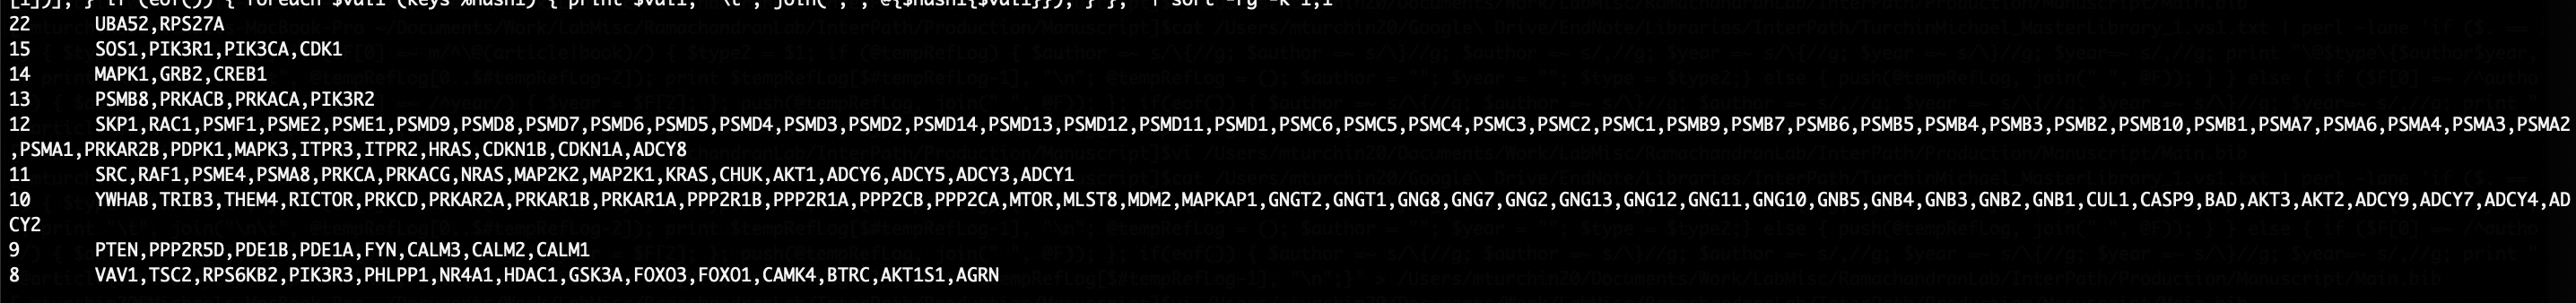
\includegraphics[scale=1]{Images/Supp/InterPath_Supp_Table_TopPathwayGeneCounts.png}
%\caption[TBD]{\textbf{Table of Most Present Genes in Significant MAPIT-R Pathways} \textcolor{red}{this will be a table}}
%\label{InterPath-Supp-Tables-GeneCounts}
%\end{figure}
%\end{landscape}
%\clearpage

\newcounter{CharNumber2}
\setcounter{CharNumber2}{1}
\renewcommand{\thetable}{\arabic{table}\alph{CharNumber2}}
\setlength{\footskip}{3cm}
\begin{landscape}
\begin{table}[ht]
\centering
\hspace*{-1.75cm}
\begin{tabular}{ccl}
  \hline
\textbf{Population} & \textbf{Gene Count} & \textbf{Genes} \\
  \hline
 \textbf{African} & & \\
 & 11 & MAPK3,MAPK1 \\
  & 10 & TNF \\
  &  9 & PRKCB,PLCB4,PLCB3,PLCB2,PLCB1,HRAS \\
  &  8 & RAF1,PRKCG,PRKCA,NRAS,MAP2K1,KRAS,HLA-G,HLA-E,HLA-DRB1,HLA-DRA,HLA-DQB1, \\
  & & HLA-DQA2,HLA-DQA1,HLA-DPB1,HLA-DPA1,HLA-DOB,HLA-DOA,HLA-DMB,HLA-DMA, \\
  & & HLA-C,HLA-B,HLA-A \\
  &  7 & PRKACG,PRKACB,PRKACA,MAP2K2,ITPR1,HLA-F,FAS,CD86,CD80,CD28,CACNA1C,BRAF \\
  &  6 & RAC2,RAC1,PRF1,PIK3R5,PIK3R3,PIK3R2,PIK3R1,PIK3CG,PIK3CD,PIK3CB,PIK3CA,ITPR3, \\ 
  & & ITPR2,IL2,IFNG,GNAQ,FASLG,CD40,CALML6,CALML5,CALML3,CALM3,CALM2,CALM1, \\
  & & CACNA1D,ADCY8,ADCY3,ADCY1 \\
  &  5 & SOS2,SOS1,ROCK2,ROCK1,RHOA,RAC3,PPP3R1,PPP3CC,PPP3CB,PPP3CA,PDGFRA,ITGB7, \\ 
  & & ITGB1,ITGA4,IL10,GZMB,EGFR,EGF,CXCR4,CHP2,CACNA1S,ADCY9,ADCY7,ADCY6, \\
  & & ADCY5,ADCY4,ADCY2,ACTG1,ACTB \\
  \\
  \textbf{Caribbean} & & \\
  & 6 & ITGB1 \\
  \\
  \textbf{Chinese} & & \\
  & 5 & HLA-DRB5,HLA-DRB1,HLA-DRA,HLA-DQB1,HLA-DQA2,HLA-DQA1,HLA-DPB1,HLA-DPA1, \\
  & & HLA-DOB,HLA-DOA,HLA-DMB,HLA-DMA \\
   \hline
\end{tabular}
\caption[TBD]{\textbf{MAPIT-R Genome-Wide Significant Pathway Gene Counts: KEGG Height}. Caption continued at end of tables.}
\label{InterPath-Supp-Tables-AllPops-TopGeneCounts-KEGG-Height-a}
\end{table}
\clearpage
\addtocounter{table}{-1}
\addtocounter{CharNumber2}{1}

\begin{table}[ht]
\centering
\vspace*{-1.cm}
\hspace*{-1.75cm}
\begin{tabular}{ccl}
  \hline
\textbf{Population} & \textbf{Gene Count} & \textbf{Genes} \\
  \hline
  \textbf{African} & & \\
  & 18 & MAPK3,MAPK1 \\
  & 14 & PIK3CG,PIK3CD,PIK3CB,PIK3CA,HRAS \\
  & 13 & RAF1,PIK3R5,PIK3R3,PIK3R2,PIK3R1,NRAS,MAP2K1,KRAS \\
  & 12 & TNF,PRKCB,MAP2K2 \\
  & 11 & SOS2,SOS1 \\
  & 10 & PRKCG,PRKCA,HLA-DRB1,HLA-DRA,HLA-DQB1,HLA-DQA2,HLA-DQA1,HLA-DPB1,HLA-DPA1, \\
  & & HLA-DOB,HLA-DOA,HLA-DMB,HLA-DMA,GSK3B,GRB2,BRAF \\
  &  9 & TP53,RHOA,RAC1,PLCB4,PLCB3,PLCB2,PLCB1,ITGB1,CCND1,AKT3,AKT2,AKT1 \\
  &  8 & RAC2,PRKACG,PRKACB,PRKACA,PLCG1,ITGA4,IL10,IFNG,HLA-G,HLA-E,HLA-C,HLA-B, \\
  & & HLA-A,EP300,EGFR,CREBBP,CDC42,CD28 \\
  &  7 & PLCG2,IL4,IL2,HLA-F,FAS,EGF,CD86,CD80,CASP9,CAMK2G,CAMK2D,CAMK2B,CAMK2A, \\ 
  & & CALML6,CALML5,CALML3,CALM3,CALM2,CALM1,CACNA1C,ADCY8,ADCY3,ADCY1, \\
  & & ACTG1,ACTB \\
  &  6 & ROCK2,ROCK1,RELA,RAC3,PTK2,PRF1,PPP3R1,PPP3CC,PPP3CB,PPP3CA,PAK1,NFKBIA, \\ 
  & & NFKB1,LAMA2,ITGB7,ITGAV,ITGA6,ITGA3,ITGA2B,ITGA2,IL5,IKBKB,GNAQ,FASLG, \\
  & & CTNNB1,CHP2,CDK4,CD40,CACNA1D,ADCY9,ADCY7,ADCY6,ADCY5,ADCY4,ADCY2 \\
  &  5 & VAV3,VAV2,VAV1,TGFB1,TCF7L2,TCF7L1,TCF7,SHC4,SHC3,SHC2,SHC1,RB1,PTPN6,PTEN, \\ 
  & & PDGFRA,MYC,MDM2,MAPK9,LEF1,JUN,ITPR1,ITGB8,ITGB6,ITGB5,ITGB4,ITGB3,ITGB2, \\ 
  & & ITGA9,ITGA8,ITGA7,ITGA11,ITGA10,ITGA1,IGF1,GZMB,GNAI3,GNAI1,FYN,E2F3,E2F2,E2F1, \\ 
  & & DAG1,CYCS,CXCR4,CDKN1A,CDK6,CASP3,CACNA1S,BAD,ACTN4,ACTN3,ACTN2,ACTN1,ABL1 \\ 
  \\
  \textbf{Chinese} & & \\
  & 7 & HLA-DRB5,HLA-DRB1,HLA-DRA,HLA-DQB1,HLA-DQA2,HLA-DQA1,HLA-DPB1,HLA-DPA1, \\ 
  & & HLA-DOB,HLA-DOA,HLA-DMB,HLA-DMA \\
  &  6 & TNF \\
  &  5 & IFNG,HLA-G,HLA-F,HLA-E,HLA-C,HLA-B,HLA-A,CD86,CD80,CD28 \\
   \hline
\end{tabular}
\caption[TBD]{\textbf{MAPIT-R Genome-Wide Significant Pathway Gene Counts: KEGG BMI}}
\label{InterPath-Supp-Tables-AllPops-TopGeneCounts-KEGG-BMI-a}
\end{table}
\clearpage
\addtocounter{table}{-1}
\addtocounter{CharNumber2}{1}

\begin{table}[ht]
\centering
\vspace*{0cm}
\hspace*{-1.75cm}
\begin{tabular}{ccl}
  \hline
\textbf{Population} & \textbf{Gene Count} & \textbf{Genes} \\
  \hline
  \textbf{African} & & \\
   & 8 & MAPK1 \\
    & 7 & PIK3R2,PIK3R1,PIK3CA \\
    & 6 & SOS1,MAPK3,MAP2K2,MAP2K1,GRB2,CREB1,CDK1 \\
    & 5 & UBA52,RPS27A,RAF1,PRKCD,PRKACB,PPP2R5D,PPP2R1B,PPP2R1A,PPP2CB, \\
    & & PPP2CA,ITPR3,ITPR2,ITGB1,HRAS,GNGT2,GNGT1,GNG8,GNG7,GNG2,GNG13, \\ 
    & & GNG12,GNG11,GNG10,GNB5,GNB4,GNB3,GNB2,GNB1 \\
   \hline
\end{tabular}
\caption[TBD]{\textbf{MAPIT-R Genome-Wide Significant Pathway Gene Counts: REACTOME Height}}
\label{InterPath-Supp-Tables-AllPops-TopGeneCounts-REACTOME-Height-a}
\end{table}
\clearpage
\addtocounter{table}{-1}
\addtocounter{CharNumber2}{1}

\begin{table}[ht]
\centering
\vspace*{-2cm}
\hspace*{-2cm}
\begin{tabular}{ccl}
  \hline
\textbf{Population} & \textbf{Gene Count} & \textbf{Genes} \\
  \hline
  \textbf{African} & & \\
  & 22 & UBA52,RPS27A \\
  & 15 & SOS1,PIK3R1,PIK3CA,CDK1 \\
  & 14 & MAPK1,GRB2,CREB1 \\
  & 13 & PSMB8,PRKACB,PRKACA,PIK3R2 \\
  & 12 & SKP1,RAC1,PSMF1,PSME2,PSME1,PSMD9,PSMD8,PSMD7,PSMD6,PSMD5,PSMD4,PSMD3, \\
  & & PSMD2,PSMD14,PSMD13,PSMD12,PSMD11,PSMD1,PSMC6,PSMC5,PSMC4,PSMC3,PSMC2, \\ 
  & & PSMC1,PSMB9,PSMB7,PSMB6,PSMB5,PSMB4,PSMB3,PSMB2,PSMB10,PSMB1,PSMA7, \\
  & & PSMA6,PSMA4,PSMA3,PSMA2,PSMA1,PRKAR2B,PDPK1,MAPK3,ITPR3,ITPR2,HRAS, \\
  & & CDKN1B,CDKN1A,ADCY8 \\
  & 11 & SRC,RAF1,PSME4,PSMA8,PRKCA,PRKACG,NRAS,MAP2K2,MAP2K1,KRAS,CHUK,AKT1, \\
  & & ADCY6,ADCY5,ADCY3,ADCY1 \\
  & 10 & YWHAB,TRIB3,THEM4,RICTOR,PRKCD,PRKAR2A,PRKAR1B,PRKAR1A,PPP2R1B, \\ 
  & & PPP2R1A,PPP2CB,PPP2CA,MTOR,MLST8,MDM2,MAPKAP1,GNGT2,GNGT1,GNG8,GNG7, \\
  & & GNG2,GNG13,GNG12,GNG11,GNG10,GNB5,GNB4,GNB3,GNB2,GNB1,CUL1,CASP9,BAD,AKT3, \\
  & & AKT2,ADCY9,ADCY7,ADCY4,ADCY2 \\
    & 9 & PTEN,PPP2R5D,PDE1B,PDE1A,FYN,CALM3,CALM2,CALM1 \\
    & 8 & VAV1,TSC2,RPS6KB2,PIK3R3,PHLPP1,NR4A1,HDAC1,GSK3A,FOXO3,FOXO1,CAMK4,BTRC, \\ 
    & & AKT1S1,AGRN \\
    & 7 & RPA3,RPA2,RPA1,RBX1,PRKCG,PRKCE,NCAN,CDK2 \\
    & 6 & TRIO,SHC1,SEH1L,SDC4,SDC3,SDC2,SDC1,RANBP2,PLCG1,PLCB3,PLCB2,PLCB1,PIK3CB, \\ 
    & & ORC5,ORC4,ORC3,ORC2,ORC1,NUP85,NUP43,NUP37,NUP133,NUP107,MYC,MCM8,MCM7, \\
    & & MCM6,MCM5,MCM4,MCM3,MCM2,LCK,KALRN,HSPG2,GPC6,GPC5,GPC2,GPC1,GNAS, \\ 
    & & GNAI2,GNAI1,E2F3,E2F1,CDC6,CDC42,ADAM17 \\  
    & 5 & YES1,WEE1,VCAN,STAT5B,STAT5A,STAT3,STAG1,SMC3,SAA1,RELA,RASGRF2,RASGRF1, \\
    & & RAD21,PTPN6,PSEN2,PSEN1,PRIM2,PRIM1,POLE2,POLE,POLA2,PLA2G4A,PAK2,NCSTN, \\
    & & MNAT1,MCM10,MAPK8,MAPK14,ITGB3BP,IKBKB,HIST4H4,HIST2H2AA3,HIST1H4L, \\
    & & HIST1H4K,HIST1H4J,HIST1H4H,HIST1H4F,HIST1H4E,HIST1H4D,HIST1H4C,HIST1H4B, \\
    & & HIST1H4A,HIST1H2BO,HIST1H2BN,HIST1H2BM,HIST1H2BL,HIST1H2BK,HIST1H2BJ,HIST1H2BI, \\
    & & HIST1H2BH,HIST1H2BG,HIST1H2BF,HIST1H2BE,HIST1H2BD,HIST1H2BC,HIST1H2BB, \\
    & & HIST1H2AJ,HIST1H2AE,HIST1H2AD,HIST1H2AC,HIST1H2AB,HEXB,HEXA,HDAC2,H2AFZ, \\
    & & GXYLT2,GXYLT1,GRP,GCGR,FFAR1,EP300,E2F2,DCN,DBF4,CSPG4,CRK,CREBBP,CHRM3, \\
    & & CDT1,CDK7,CDC7,CDC45,CCNH,BCAN,B4GALT7,B3GAT2,B3GAT1,B3GALT6,ATR,APP, \\ 
    & & APH1B,APH1A,AP2S1,AP2M1,AP2B1,AP2A2,AP2A1 \\
   \hline
\end{tabular}
\caption[TBD]{\textbf{MAPIT-R Genome-Wide Significant Pathway Gene Counts: REACTOME BMI}}
\label{InterPath-Supp-Tables-AllPops-TopGeneCounts-REACTOME-BMI-a}
\end{table}
\clearpage
\addtocounter{table}{-1}
\addtocounter{CharNumber2}{1}
\end{landscape}
\renewcommand{\thetable}{\arabic{table}}
\setlength{\footskip}{1cm}

\begin{table} [t!]
  \caption{\textbf{MAPIT-R Genome-Wide Significant Pathway Gene Counts}. The tables show the lists of genes that appear most frequently across the pathways that were MAPIT-R genome-wide significant in the following phenotype and pathway database combinations: (a) KEGG height, (b) KEGG BMI, (c) REACTOME height, and (d) REACTOME BMI. The first columns list the UKB subsets, the second columns list the number of times the given genes appeared in the set of genome-wide significant pathways for that subset, pathway database, and phenotype combination, and the third columns list the actual gene names for each of these numbers of gene counts.}
\label{InterPath-Supp-Tables-AllPops-TopGeneCounts-Caption}
\end{table}
\clearpage

\setlength{\footskip}{2cm}
\begin{table}[ht]
\centering
\begin{tabular}{ccccc}
  \hline
  \textbf{Database} & \textbf{Gene} & \textbf{No Restriction} & \textbf{Restricted} & \textbf{-$\log_{10}$($p$-Value)} \\
  & & \textbf{$p$-Value} & \textbf{$p$-Value} & \textbf{Difference} \\
  \hline
  \textbf{KEGG:} & & & & \\
  & CDKN2A & 1.248E-01 & 7.974E-03 & 1.194 \\
  & CCNB2 & 2.795E-01 & 1.876E-02 & 1.173 \\
  & CCNB1 & 2.795E-01 & 1.876E-02 & 1.173 \\
  & PTEN & 5.340E-02 & 4.186E-03 & 1.106 \\
  & GADD45G & 6.710E-02 & 6.559E-03 & 1.010 \\
  & GADD45B & 6.710E-02 & 6.559E-03 & 1.010 \\
  & GADD45A & 6.710E-02 & 6.559E-03 & 1.010 \\
  & CHEK2 & 6.710E-02 & 6.559E-03 & 1.010 \\
  & CHEK1 & 6.710E-02 & 6.559E-03 & 1.010 \\
  & ATR & 6.710E-02 & 6.559E-03 & 1.010 \\
  \\
  \textbf{REACTOME:} & & & & \\ 
  & SMC3 & 1.456E-05 & 5.589E-09 & 3.416 \\
  & PSM* & 5.304E-04 & 4.464E-06 & 2.075 \\
  & (Cluster) & & & \\ 
  & FBXW11 & 7.902E-02 & 1.956E-03 & 1.606 \\
  & NFKBIE & 2.702E-02 & 1.956E-03 & 1.140 \\
  & PRKCB & 2.204E-01 & 1.797E-02 & 1.089 \\
  & MALT1 & 7.902E-02 & 1.109E-02 & 0.853 \\
  & LOC646626 & 7.902E-02 & 1.109E-02 & 0.853 \\
  & CARD11 & 7.902E-02 & 1.109E-02 & 0.8.53 \\
  & BCL10 & 7.902E-02 & 1.109E-02 & 0.8.53 \\
  & ATR & 8.004E-03 & 1.261E-03 & 0.8.02 \\
   \hline
\end{tabular}
\caption[TBD]{\textbf{MAPIT-R Genome-Wide Significant Pathway Gene Counts: Hypergeometric Enrichment Size Restricted Examples}. The table shows the top examples of genes that became more significant in the hypergeometric enrichment analyses after the size restriction step in both pathway databases. Results are only shown for BMI since the majority of genome-wide significant pathways in height were lost from the size restriction step alone. The first column lists the pathway database, the second column lists the genes, the third column lists the original, unrestricted hypergeometric enrichment $p$-value, the fourth column lists the new, size-restricted hypergeometric enrichment $p$-value, and the fifth column lists the -$\log_{10}$ $p$-value difference between the third and fourth column. The top 10 genes sorted by the fifth column are shown for each database. For a plot of results from every gene analyzed in both databases, see Supplementary Figure \ref{InterPath-Supp-Figure-Hypergeometric-RestrictedComps-African-BMI}). Note that a single entry in the REACTOME results is included to represent the PSM* gene family cluster to preserve space.}
\label{InterPath-Supp-Table-Hypergeometric-RestrictedComps-African-BMI-TopExamples}
\end{table}
\clearpage
\setlength{\footskip}{1cm}

\begin{landscape}
\begin{table}[ht]
\centering
\hspace*{-1.5cm}
\begin{tabular}{ccccccc}
  \hline
  \textbf{Gene} & \textbf{Pathway SNP} & \textbf{Gene Count in} & \textbf{Total Count of} & \textbf{Gene Count in} & \textbf{Total Count of} & \textbf{Hypergeometric} \\
   & \textbf{Count Limit} & \textbf{Top Pathways} & \textbf{Top Pathways} & \textbf{All Pathways} & \textbf{All Pathways} & \textbf{$p$-Value} \\
  \hline
 \textbf{UBA52} & & & & & & \\
 & No Limit & 22 & 65 & 106 & 658 & 1.537E-4 \\
 & $<=$ 1000 SNPs & 10 & 26 & 84 & 577 & 1.855E-3 \\
\\
 \textbf{PSM*} & & & & & & \\
 & No Limit & 12 & 65 & 44 & 658 & 5.304E-4 \\
 & $<=$ 1000 SNPs & 9 & 26 & 34 & 577 & 4.464E-6 \\
   \hline
\end{tabular}
\caption[TBD]{\textbf{MAPIT-R Genome-Wide Significant Pathway Gene Counts: Hypergeometric Enrichment Examples}. Caption continued on next page.}
\label{InterPath-Supp-Tables-AllPops-TopGeneCount-HypergeometricTests}
\end{table}
\end{landscape}
\clearpage

\addtocounter{table}{-1}
\begin{table} [t!]
  \caption{\textbf{MAPIT-R Genome-Wide Significant Pathway Gene Counts: Hypergeometric Enrichment Examples}. The table shows examples and results of running the hypergeometric test for enrichment on two different genes in two different study designs. In all cases a gene is tested for being significantly more frequent among the set of MAPIT-R genome-wide significant pathways than among the background distribution of pathways in the original database. Two study designs were employed for these tests, either (a) using all pathways present in the given databases or (b) using only pathways that contained less than or equal to 1,000 SNPs. The first column lists the gene or gene family being tested. The second column lists which of the two aforementioned study designs was used. Columns three through six list the different count values used in the hypergeometric test: the third column lists the number of times a gene is present among the genome-wide significant list of pathways, the fourth column lists the total number of pathways that were genome-wide significant, the fifth column lists the number of times a gene is present among all the pathways in the given database, and the sixth column lists the total number of pathways in the given database. The seventh column is the hypergeometric $p$-value associated with columns three through six. Note that the vast majority of proteasome genes included in our analysis had the same number of gene counts across each hypergeometric category, hence why \textbf{PSM*} was used to represent them as a whole.}
\label{InterPath-Supp-Tables-AllPops-TopGeneCount-HypergeometricTests-Caption}
\end{table}
\clearpage

\begin{landscape}
\setlength{\footskip}{2cm}
\begin{table}[ht]
\centering
\begin{tabular}{lrrr}
  \hline
\textbf{Pathway} & \textbf{Genes} & \textbf{SNPs} & \textbf{$p$-Value} \\ 
  \hline
REACTOME\_M\_G1\_TRANSITION & 73 & 458 & 3.191E-06 \\ 
  REACTOME\_CELL\_CYCLE\_CHECKPOINTS & 105 & 670 & 5.781E-06 \\ 
  REACTOME\_HOST\_INTERACTIONS\_OF\_HIV\_FACTORS & 112 & 963 & 7.521E-06 \\ 
  REACTOME\_DOWNSTREAM\_SIGNALING\_EVENTS\_OF\_ & & & \\ 
  \qquad B\_CELL\_RECEPTOR\_BCR & 89 & 745 & 1.195E-05 \\
  REACTOME\_REGULATION\_OF\_APOPTOSIS & 52 & 564 & 1.218E-05 \\ 
  REACTOME\_MITOTIC\_G1\_G1\_S\_PHASES & 121 & 747 & 1.453E-05 \\ 
  REACTOME\_ACTIVATION\_OF\_NF\_KAPPAB\_IN\_B\_CELLS & 59 & 465 & 1.861E-05 \\ 
  REACTOME\_ASSEMBLY\_OF\_THE\_PRE\_REPLICATIVE\_COMPLEX & 60 & 331 & 3.293E-05 \\ 
  REACTOME\_ANTIGEN\_PROCESSING\_CROSS\_PRESENTATION & 68 & 850 & 3.956E-05 \\ 
   \hline
\end{tabular}
  \caption{\textbf{MAPIT-R Genome-Wide Significant Pathway Gene Counts: Size Restricted Proteasome Pathways}. Caption continued on next page.}
\label{InterPath-Supp-Tables-AllPops-TopGeneCount-SizeRestricted-Proteasome}
\end{table}
\clearpage
\end{landscape}
\setlength{\footskip}{1cm}

\addtocounter{table}{-1}
\begin{table} [t!]
  \caption{\textbf{MAPIT-R Genome-Wide Significant Pathway Gene Counts: Size Restricted Proteasome Pathways}. The table shows the MAPIT-R genome-wide significant REACTOME pathways for BMI in the African subset that both have SNP sizes less than 1,000 and also contain the set of proteasome genes being investigated (\textit{PSMA}*, \textit{PSMB}*, \textit{PSMC}*, \textit{PSMD}*, and \textit{PSME*}). The first column shows the REACTOME pathway names, the second column shows the number of genes that were included in the MAPIT-R analysis, the third column show the number of SNPs that were included in the MAPIT-R analysis, and the fourth column shows the MAPIT-R $p$-value.}
\label{InterPath-Supp-Tables-AllPops-TopGeneCount-SizeRestricted-Proteasome-Caption}
\end{table}
\clearpage

%\begin{figure}[htbp]
%\centering
%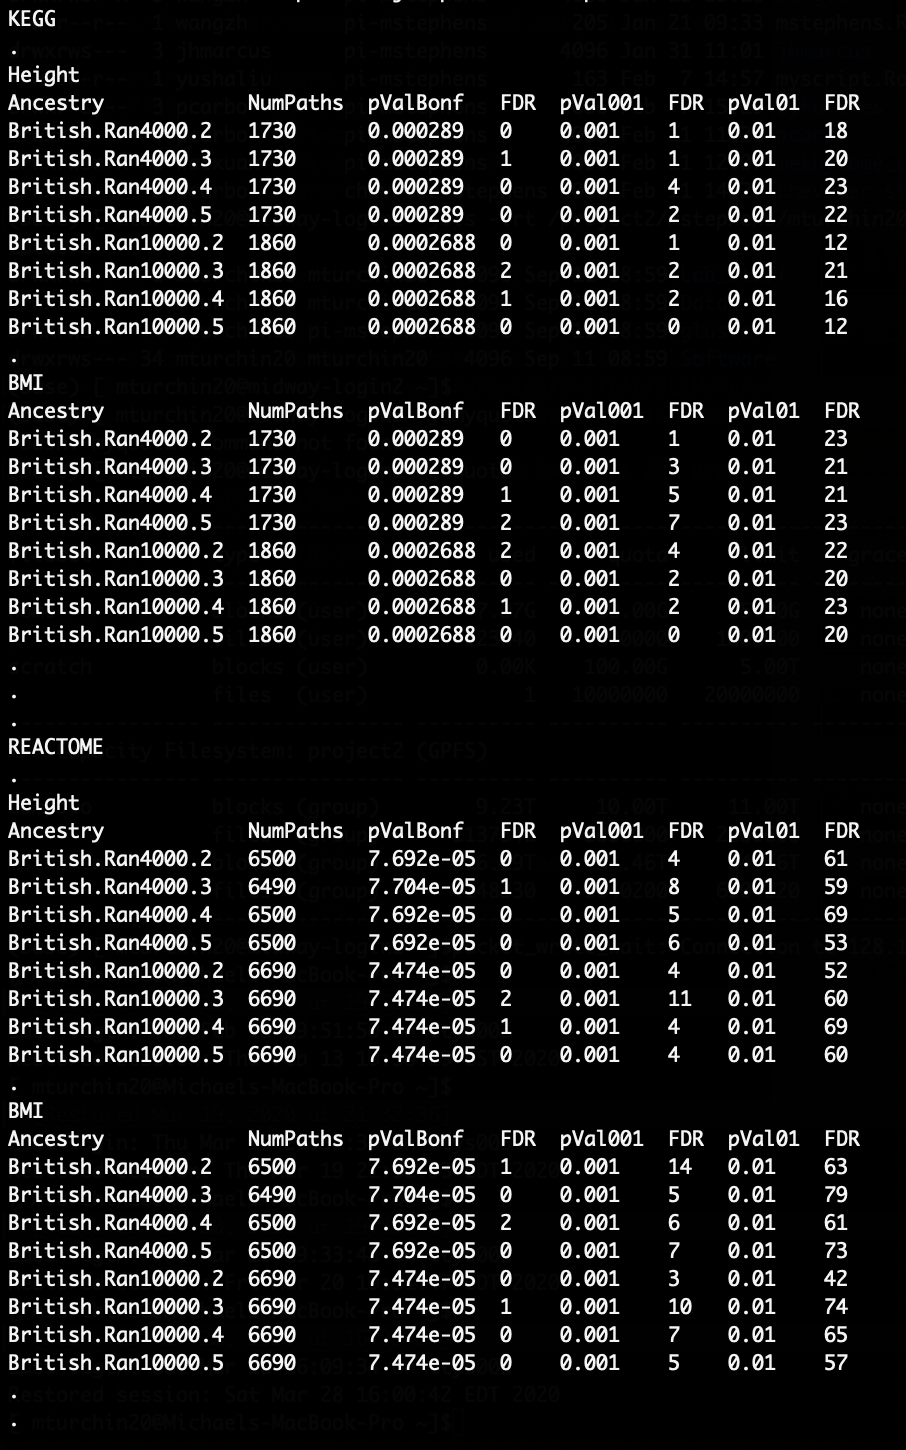
\includegraphics[scale=1.5]{Images/Supp/InterPath_Supp_Figure_FDRs_BritReps_vs1.png}
%\caption[TBD]{\textbf{TBD}. }
%\label{InterPath-Supp-Figure-BritReps-FDRs}
%\end{figure}
%\clearpage

\setlength{\footskip}{4cm}
\begin{landscape}
\begin{table}[ht]
\vspace*{-1.25cm}
\centering
\hspace*{-3.25cm}
\begin{tabular}{ccccccccccc}
  \hline
\textbf{Population} & \textbf{Pathway} & \textbf{Bonferroni} & \textbf{Bonferroni} & \textbf{Bonferroni} & \textbf{0.001} & \textbf{0.001} & \textbf{0.001} & \textbf{0.01} & \textbf{0.01} & \textbf{0.01} \\
 & \textbf{Counts} & \textbf{Threshold} & \textbf{Counts} & \textbf{FDR} & \textbf{Threshold} & \textbf{Counts} & \textbf{FDR} & \textbf{Threshold} & \textbf{Counts} & \textbf{FDR} \\ 
  \hline
\textbf{KEGG Height:} & & & & & & & & & \\
British.Ran4000 & 1730 & 2.890E-04 & 0 & 0.000 & 0.001 & 0 & 0.000 & 0.010 & 13 & 0.751 \\
  British.Ran4000.2 & 1730 & 2.890E-04 & 0 & 0.000 & 0.001 & 1 & 0.058 & 0.010 & 18 & 1.040 \\
  British.Ran4000.3 & 1730 & 2.890E-04 & 1 & 0.058 & 0.001 & 1 & 0.058 & 0.010 & 20 & 1.156 \\
  British.Ran4000.4 & 1730 & 2.890E-04 & 0 & 0.000 & 0.001 & 4 & 0.231 & 0.010 & 23 & 1.329 \\
  British.Ran4000.5 & 1730 & 2.890E-04 & 0 & 0.000 & 0.001 & 2 & 0.116 & 0.010 & 22 & 1.272 \\
  British.Ran10000.1 & 1860 & 2.688E-04 & 0 & 0.000 & 0.001 & 1 & 0.054 & 0.010 & 26 & 1.398 \\
  British.Ran10000.2 & 1860 & 2.688E-04 & 0 & 0.000 & 0.001 & 1 & 0.054 & 0.010 & 12 & 0.645 \\
  British.Ran10000.3 & 1860 & 2.688E-04 & 2 & 0.108 & 0.001 & 2 & 0.108 & 0.010 & 21 & 1.129 \\
  British.Ran10000.4 & 1860 & 2.688E-04 & 1 & 0.054 & 0.001 & 2 & 0.108 & 0.010 & 16 & 0.860 \\
  British.Ran10000.5 & 1860 & 2.688E-04 & 0 & 0.000 & 0.001 & 0 & 0.000 & 0.010 & 12 & 0.645 \\
  \\
  \textbf{KEGG BMI:} & & & & & & & & & \\
British.Ran4000 & 1730 & 2.890E-04 & 1 & 0.058 & 0.001 & 2 & 0.116 & 0.010 & 14 & 0.809 \\
  British.Ran4000.2 & 1730 & 2.890E-04 & 0 & 0.000 & 0.001 & 1 & 0.058 & 0.010 & 23 & 1.329 \\
  British.Ran4000.3 & 1730 & 2.890E-04 & 0 & 0.000 & 0.001 & 3 & 0.173 & 0.010 & 21 & 1.214 \\
  British.Ran4000.4 & 1730 & 2.890E-04 & 1 & 0.058 & 0.001 & 5 & 0.289 & 0.010 & 21 & 1.214 \\
  British.Ran4000.5 & 1730 & 2.890E-04 & 2 & 0.116 & 0.001 & 7 & 0.405 & 0.010 & 23 & 1.329 \\
  British.Ran10000.1 & 1860 & 2.688E-04 & 0 & 0.000 & 0.001 & 1 & 0.054 & 0.010 & 25 & 1.344 \\
  British.Ran10000.2 & 1860 & 2.688E-04 & 2 & 0.108 & 0.001 & 4 & 0.215 & 0.010 & 22 & 1.183 \\
  British.Ran10000.3 & 1860 & 2.688E-04 & 0 & 0.000 & 0.001 & 2 & 0.108 & 0.010 & 20 & 1.075 \\
  British.Ran10000.4 & 1860 & 2.688E-04 & 1 & 0.054 & 0.001 & 2 & 0.108 & 0.010 & 23 & 1.237 \\
  British.Ran10000.5 & 1860 & 2.688E-04 & 0 & 0.000 & 0.001 & 0 & 0.000 & 0.010 & 20 & 1.075 \\
   \hline
\end{tabular}
\caption[TBD]{\textbf{MAPIT-R Results: British Replicates Phenotype Permutation FDRs}. Caption continued at end of tables.}
\label{InterPath-Supp-Tables-BritReps-FDRs-pt1}
\end{table}
\end{landscape}
\clearpage
\setlength{\footskip}{1cm}
\addtocounter{table}{-1}

\setlength{\footskip}{4cm}
\renewcommand{\thetable}{\arabic{table}}
\begin{landscape}
\begin{table}[ht]
\vspace*{-1.25cm}
\centering
\hspace*{-3.5cm}
\begin{tabular}{ccccccccccc}
  \hline
\textbf{Population} & \textbf{Pathway} & \textbf{Bonferroni} & \textbf{Bonferroni} & \textbf{Bonferroni} & \textbf{0.001} & \textbf{0.001} & \textbf{0.001} & \textbf{0.01} & \textbf{0.01} & \textbf{0.01} \\
 & \textbf{Counts} & \textbf{Threshold} & \textbf{Counts} & \textbf{FDR} & \textbf{Threshold} & \textbf{Counts} & \textbf{FDR} & \textbf{Threshold} & \textbf{Counts} & \textbf{FDR} \\ 
  \hline
  \textbf{REACTOME Height:} & & & & & & & & & \\
British.Ran4000 & 6500 & 7.692E-05 & 0 & 0.000 & 0.001 & 9 & 0.138 & 0.010 & 69 & 1.062 \\
  British.Ran4000.2 & 6500 & 7.692E-05 & 0 & 0.000 & 0.001 & 4 & 0.062 & 0.010 & 61 & 0.938 \\
  British.Ran4000.3 & 6490 & 7.704E-05 & 1 & 0.015 & 0.001 & 8 & 0.123 & 0.010 & 59 & 0.909 \\
  British.Ran4000.4 & 6500 & 7.692E-05 & 0 & 0.000 & 0.001 & 5 & 0.077 & 0.010 & 69 & 1.062 \\
  British.Ran4000.5 & 6500 & 7.692E-05 & 0 & 0.000 & 0.001 & 6 & 0.092 & 0.010 & 53 & 0.815 \\
   British.Ran10000.1 & 6690 & 7.474E-05 & 0 & 0.000 & 0.001 & 4 & 0.060 & 0.010 & 55 & 0.822 \\
  British.Ran10000.2 & 6690 & 7.474E-05 & 0 & 0.000 & 0.001 & 4 & 0.060 & 0.010 & 52 & 0.777 \\
  British.Ran10000.3 & 6690 & 7.474E-05 & 2 & 0.030 & 0.001 & 11 & 0.164 & 0.010 & 60 & 0.897 \\
  British.Ran10000.4 & 6690 & 7.474E-05 & 1 & 0.015 & 0.001 & 4 & 0.060 & 0.010 & 69 & 1.031 \\
  British.Ran10000.5 & 6690 & 7.474E-05 & 0 & 0.000 & 0.001 & 4 & 0.060 & 0.010 & 60 & 0.897 \\

  \\
  \textbf{REACTOME BMI:} & & & & & & & & & \\
British.Ran4000 & 6490 & 7.704E-05 & 1 & 0.015 & 0.001 & 4 & 0.062 & 0.010 & 52 & 0.801 \\
  British.Ran4000.2 & 6500 & 7.692E-05 & 1 & 0.015 & 0.001 & 14 & 0.215 & 0.010 & 63 & 0.969 \\
  British.Ran4000.3 & 6490 & 7.704E-05 & 0 & 0.000 & 0.001 & 5 & 0.077 & 0.010 & 79 & 1.217 \\
  British.Ran4000.4 & 6500 & 7.692E-05 & 2 & 0.031 & 0.001 & 6 & 0.092 & 0.010 & 61 & 0.938 \\
  British.Ran4000.5 & 6500 & 7.692E-05 & 0 & 0.000 & 0.001 & 7 & 0.108 & 0.010 & 73 & 1.123 \\
  British.Ran10000.1 & 6690 & 7.474E-05 & 2 & 0.030 & 0.001 & 10 & 0.149 & 0.010 & 73 & 1.091 \\
  British.Ran10000.2 & 6690 & 7.474E-05 & 0 & 0.000 & 0.001 & 3 & 0.045 & 0.010 & 42 & 0.628 \\
  British.Ran10000.3 & 6690 & 7.474E-05 & 1 & 0.015 & 0.001 & 10 & 0.149 & 0.010 & 74 & 1.106 \\
  British.Ran10000.4 & 6690 & 7.474E-05 & 0 & 0.000 & 0.001 & 7 & 0.105 & 0.010 & 65 & 0.972 \\
  British.Ran10000.5 & 6690 & 7.474E-05 & 0 & 0.000 & 0.001 & 5 & 0.075 & 0.010 & 57 & 0.852 \\
   \hline
\end{tabular}
\caption[TBD]{\textbf{MAPIT-R Results: British Replicates Phenotype Permutation FDRs}. Continued.}
\label{InterPath-Supp-Tables-BritReps-FDRs-pt2}
\end{table}
\end{landscape}
\clearpage
\setlength{\footskip}{1cm}

\addtocounter{table}{-1}
\begin{table} [t!]
  \caption{\textbf{MAPIT-R Results: British Replicates Phenotype Permutation FDRs}. The tables show for various significance thresholds the false discovery rates observed from MAPIT-R when run on ten rounds of phenotype permutations for each British replicate subsample and pathway database. The first column lists the pathway database, phenotype, and British replicate subsample combinations. The second column lists the total number of pathways that were tested across each of the ten phenotype permutations. The third column shows the $p$-value threshold associated with using the Bonferroni method of correction, also known as the `genome-wide significant' threshold. The fourth column shows the number of pathways across all ten phenotype permutation rounds that crossed this Bonferroni threshold. The fifth column shows the associated FDR associated with the fourth column. And the remaining six columns show the same setup as columns three to five but with a $p$-value threshold of either 0.001 or 0.01.}
\label{InterPath-Supp-Tables-BritReps-FDRs-Caption}
\end{table}
\clearpage

\begingroup
\bibliographystyle{apalike}
\setstretch{1.0}
\bibliography{Main}
\endgroup


\iffalse

SCRAP

Additionally, it is unlikely that, even if such an ascertainment bias existed, it could continually be directionality consistent across pathways that span the genome. If this were an approach that aggregated single SNP tests, then directionality would not be an issue and one might become concerned about continually incorporating a persistent signal from ascertainment bias; however, because this is a joint test on multiple SNPs as once, it is far less likely that differences between genotype chip SNP distributions and non-European population SNP distributions tracts in exactly the same direction across the entire genome.

\subsubsection{Pairwise SNP Epistasis}

Our first approach to investigate SNP-level epistasis was to run the canonical pair-wise interaction model as employed by PLINK's \texttt{--epistasis} method \citep{Purcell2007} (see Online Methods and Supplementary Note for details). Here, we directly estimated the effect size of every possible SNP pairwise interaction and calculated whether it was statistically significant or not.  

Running this method on each of our four UKB population subsets, we chose to look at the 'proportion of marginally significant tests' per SNP, where marginal significance is defined as any test with a $p$-value < $1\times10^{-4}$ (Figure \ref{InterPath-Supp-Figure-PLINK}). We chose to look at proportion of tests due the varying number of SNPs across each population subset. What we find is that indeed there is variation between human ancestries in the amount of pairwise SNP epistasis across the genome. We also find that both the African and Caribbean population subsets show greater proportions of marginal interactions than the British population subset despite both non-European populations having lower sample sizes. 

\begin{figure}[t]
\centering
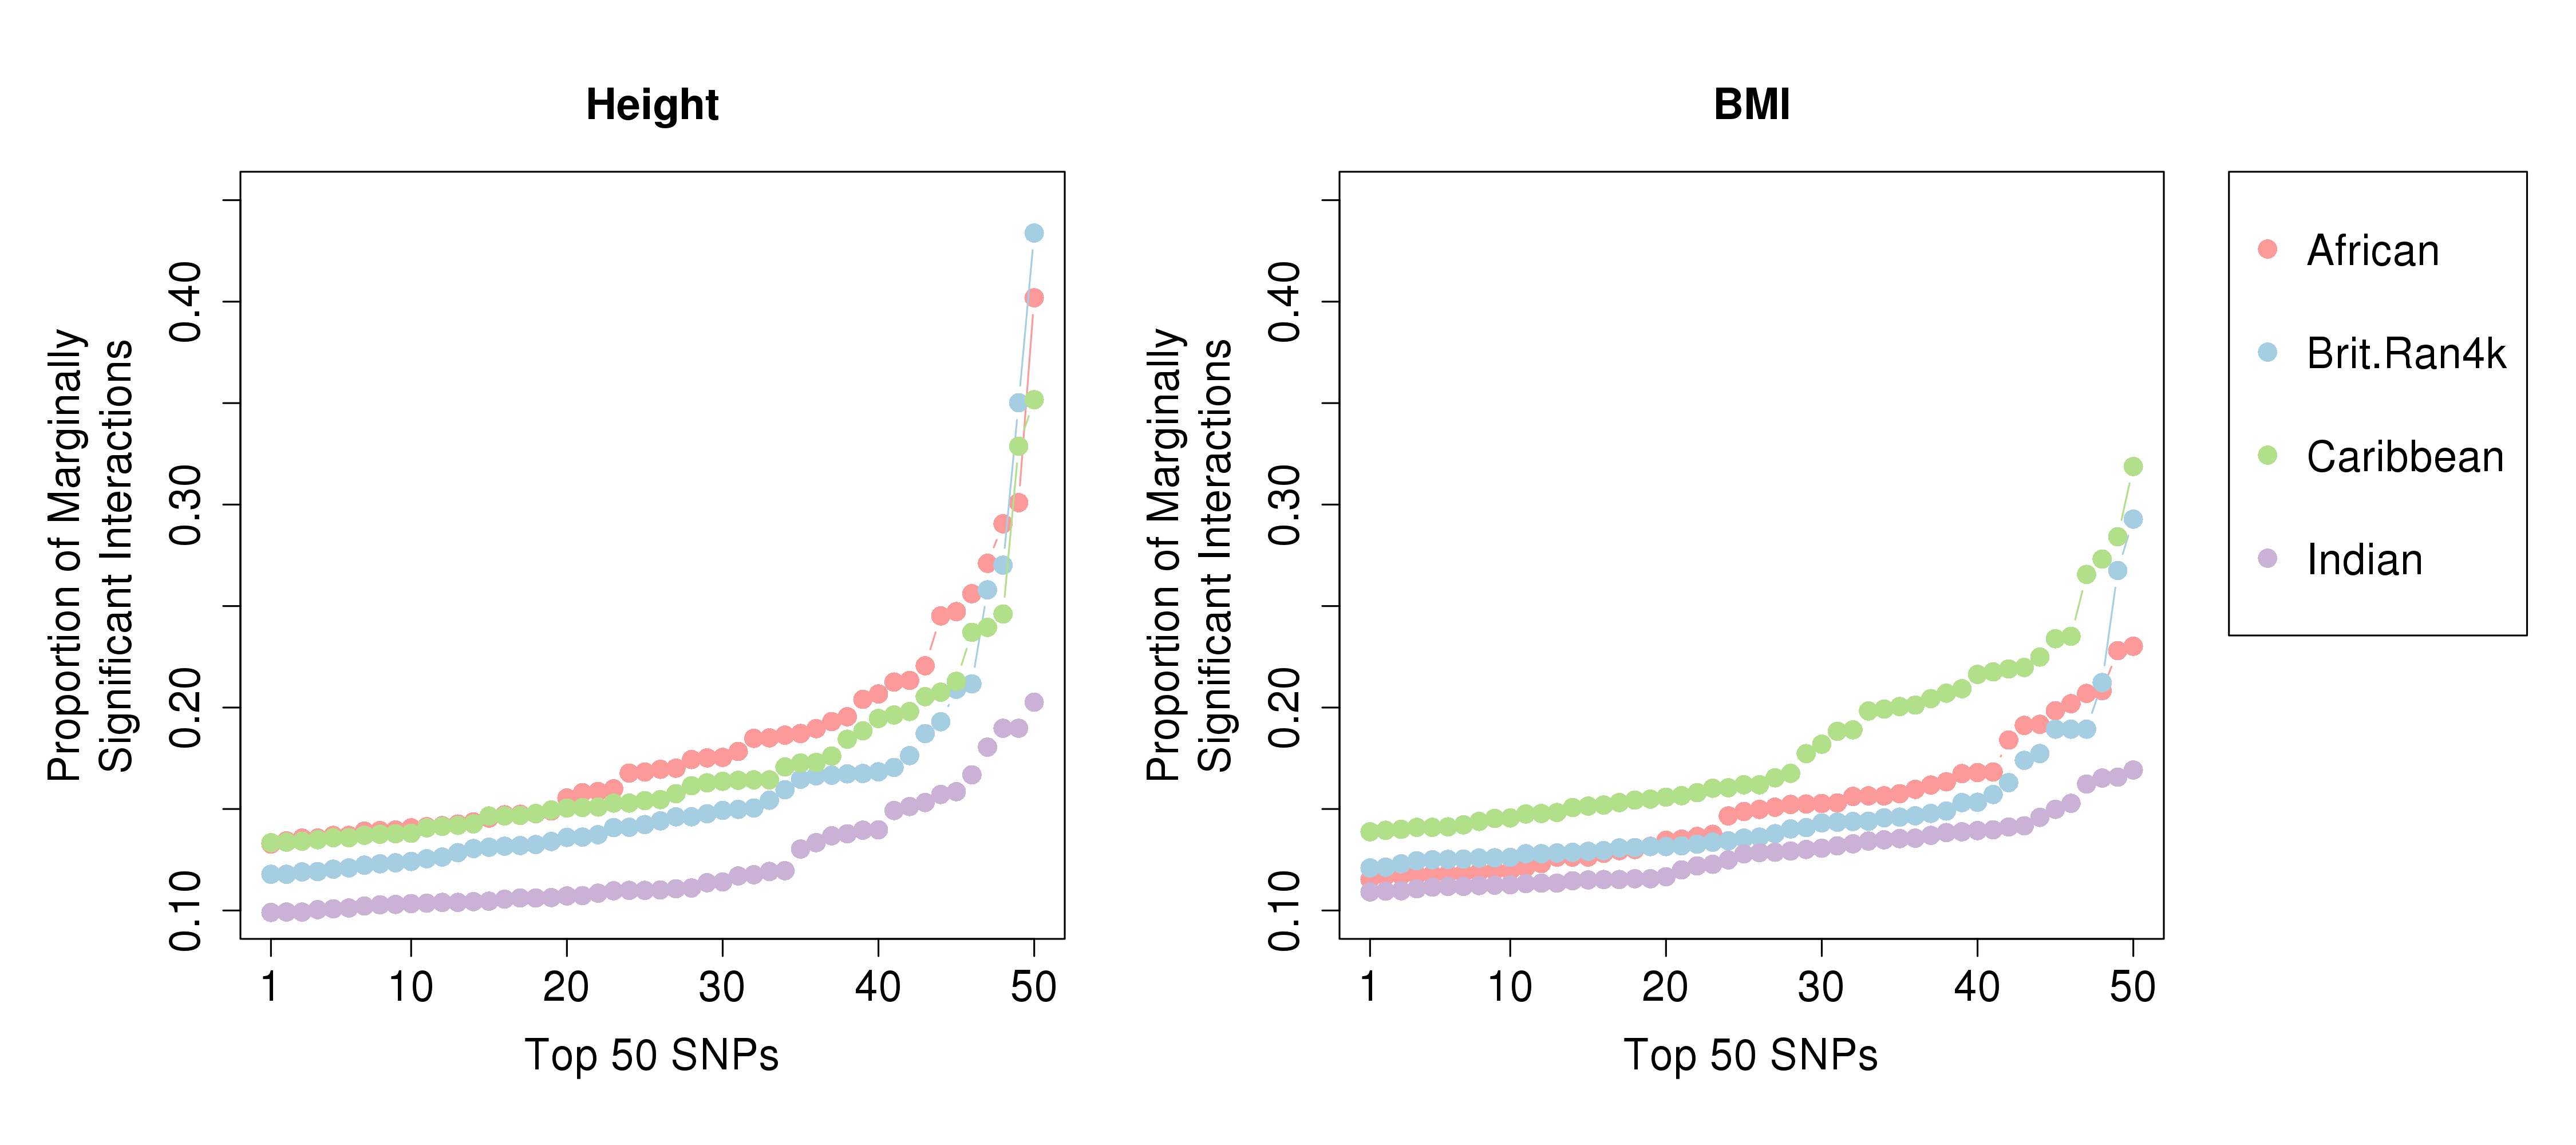
\includegraphics[scale=.35]{Images/Supp/InterPath_Supp_Figure_PLINK_vs2.png}
\caption[PLINK SNP Pairwise Epistasis]{\textbf{PLINK SNP Pairwise Epistasis.} \\ Shown are results from running PLINK's SNP-by-SNP pairwise epistasis method, \texttt{--epistasis}, on four of our initial UKB human population subsets in height and BMI. Specifically the $y$-axis shows the proportion of marginally significant interactions found per-SNP, where marginal significance is defined as the epistastic test returning a $p$-value $<$ $1\times10^{-4}$, and the $x$-axis shows the top 50 SNPs for this metric in each of the population subsets. The African subset contained 374,466 total SNPs, the British Random 4k subset contained 600,006 total SNPs, the Caribbean subset contained 410,017 total SNPs, and the Indian subset contained 505,854 total SNPs. We observe across each population different levels of marginal pairwise SNP significance as well as different patterns of significance. Additionally, both the African and Caribbean subsets contain the strongest signals.}
\label{InterPath-Supp-Figure-PLINK}
\end{figure}







\subsection{Genome Level Epistasis}\label{InterPath-Results-GenomeEpistasis}

To investigate epistasis in multiple human populations, we first extracted a variety of human ancestries from the UKB (see Online Methods). We collected a total of 8 UKB subsets with an average sample size of XXXX among the non-European populations (Supplementary Table 1), including African, Indian, Chinese, and Pakistani subsets. To maximize our sample sizes per subset, we focused on height and body mass index (BMI) as our complex traits of interest. 

The first approach we took to investigate epistasis was to look at genome-wide estimates of phenotypic PVE. Specifically, we setup a linear mixed model that incorporated both additive and epistatic interactions, and fit each of these variance components using GEMMA \citep{Zhou2012} (see Online Methods and Supplementary Note for details). Calculating these variance component PVEs for height and BMI in each of our populations, we indeed find differences across each human ancestry (Table 1).

\begin{figure}[ht]
\centering
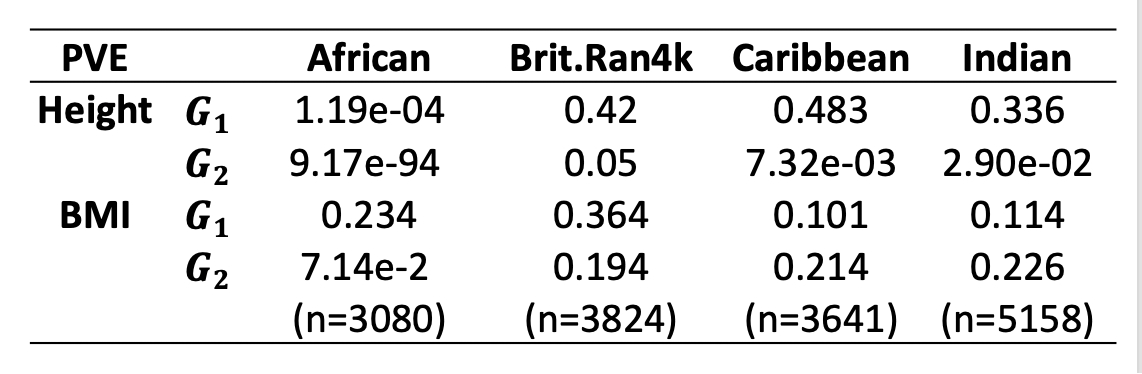
\includegraphics[scale=1]{Images/Table1_Placeholder.png}
\caption[TBD]{\textbf{TBD}. \\ this will be a table not a figure.}
\label{IntrePath-Main-Table-GEMMA}
\end{figure}

In height, we do not see anything immediately new. For the additive effects $G_1$ we mainly calculate PVEs across each population within our range of expectation (between XX and XX (citation)). Additionally, we do not currently see much evidence for second-order effects $G_2$. However, looking at BMI we see a different result. Across all populations we see non-trivial PVEs for $G_2$, ranging from XX to XX. We also see larger values in multiple non-European populations. In particular we see a particularly strong result in XXX. This might be beginning evidence that indeed, non-European populations have more potential for picking up signals of higher-order interactions in the genome.   

\fi

\end{document}
